\part{Statistical Learning and Deep Learning}

Statistical learning studies prediction rules, representation maps, and trained systems as mathematical objects.  The statistical foundations of Parts 15 and 16 remain the language for experiments, inference, and model assessment; here the emphasis is on risk, generalization, optimization, architectures, and evaluation of learned predictors.

\section{Learning Problems and Risk}

\subsection{Prediction, Loss Functions, and Risk}

A learning problem turns observations into an action rule.  Unlike inferential problems, the primary object is often the future loss of a predictor rather than a confidence statement about a parameter.

\begin{definition} \label{def:sl-prediction-problem-risk} \hlt{Prediction Problem and Risk}\\
 Inputs lie in $(\mathcal{X},\mathcal{A})$, outputs in $(\mathcal{Y},\mathcal{B})$, and $(X,Y)\sim P$ on $\mathcal{X}\times\mathcal{Y}$. Let $(\mathcal{A}_0,\mathcal{C})$ be an action space.
\begin{enumerate}[label=(\roman*)]
\setlength{\itemsep}{0pt}
\item \hlt{Predictor}: A predictor is a measurable map $f:\mathcal{X}\to\mathcal{A}_0$.
\item \hlt{Loss and risk}: For loss $\ell:\mathcal{A}_0\times\mathcal{Y}\to[0,\infty]$, define $R(f)\defeq\mathbb{E}_{P}\ell(f(X),Y)$.
\item \hlt{Bayes risk}: $R^*\defeq\inf_fR(f)$, over measurable $f:\mathcal{X}\to\mathcal{A}_0$.
\end{enumerate}
\end{definition}

\begin{definition} \label{def:sl-supervised-learning-terminology} \hlt{Supervised Learning Terminology}\\
Let $S\defeq\{(x_i,y_i):1\leq i\leq n\}$ with $x_i=(x_{i1},\ldots,x_{ip})^\top\in\mathcal{X}$ and $y_i\in\mathcal{Y}$.
\begin{enumerate}[label=(\roman*)]
\setlength{\itemsep}{0pt}
\item \hlt{Features}: Coordinates $x_{ij}$ are variables, inputs, predictors, independent variables, or features.
\item \hlt{Response}: Values $y_i$ are outputs, responses, targets, or dependent variables.
\item \hlt{Regression}: If $\mathcal{Y}\subseteq\R^q$, the task is quantitative prediction.
\item \hlt{Classification}: If $\mathcal{Y}=\mathcal{G}$ is a finite unordered label set, the task is classification.
\item \hlt{Ordered labels}: If $\mathcal{Y}$ is ordered categorical, order matters but arithmetic on labels usually does not.
\item \hlt{One-hot coding}: For $|\mathcal{G}|=K$, encode class $g$ by $t_g\in\{0,1\}^K$ with $(t_g)_g=1$.\\
Classify vector scores $s(x)\in\R^K$ by $\operatorname*{argmax}_k s_k(x)$.
\end{enumerate}
If $y_i$ are unobserved, the problem is unsupervised and targets structure in $\{x_i\}_{i=1}^n$.
\end{definition}

\begin{example} \label{ex:sl-source-learning-problems} \hlt{Representative Learning Problems}
\begin{enumerate}[label=(\roman*)]
\setlength{\itemsep}{0pt}
\item \hlt{Email filtering}: $x$ contains word and punctuation frequencies, $y\in\{\operatorname{spam},\operatorname{ham}\}$, and asymmetric loss can penalize false deletion more than missed spam.
\item \hlt{Clinical regression}: $y=\log(\mathrm{PSA})$ and $x$ contains log cancer volume, prostate weight, age, and related measurements; correlated predictors are common.
\item \hlt{Digit recognition}: $x\in[0,1]^{16\times16}$ or $[0,1]^{256}$ and $y\in\{0,\ldots,9\}$; action set may add rejection option $\bot$.
\item \hlt{Microarrays}: An expression matrix $X\in\R^{G\times n}$ has genes as rows and samples as columns.\\
Typical first tasks are unsupervised clustering of genes or samples.
\end{enumerate}
\end{example}

\begin{example} \label{ex:sl-standard-losses} \hlt{Common Prediction Losses}
\begin{enumerate}[label=(\roman*)]
\setlength{\itemsep}{0pt}
\item Regression commonly uses squared loss $\ell(a,y)=\norm{a-y}_2^2$ or absolute loss $\ell(a,y)=\abs{a-y}$.
\item Binary classification with labels in $\{-1,1\}$ uses zero-one loss $\mathbf{1}_{\{ay\leq0\}}$ for a signed score $a$.
\item Probabilistic classification uses log loss $-\log q_y$ when $q$ is a predicted distribution on labels.
\end{enumerate}
\end{example}

\begin{definition} \label{def:sl-bayes-predictor} \hlt{Bayes Predictors}
\begin{enumerate}[label=(\roman*)]
\setlength{\itemsep}{0pt}
\item \hlt{Conditional risk}: For action $a$, set $r_x(a)\defeq\mathbb{E}[\ell(a,Y)\mid X=x]$; any $f^*(x)\in\operatorname*{argmin}\limits_a r_x(a)$ is Bayes.
\item \hlt{Squared loss}: If $\ell(a,y)=(a-y)^2$ and $\mathbb{E}[|Y|\mid X=x]<\infty$, then $f^*(x)=\mathbb{E}[Y\mid X=x]$.
\item \hlt{Absolute loss}: If $\ell(a,y)=|a-y|$, any conditional median $m(x)$\\
with $\mathbb{P}(Y\leq m(x)\mid X=x)\geq\frac12$ and $\mathbb{P}(Y\geq m(x)\mid X=x)\geq\frac12$ is Bayes.
\item \hlt{Zero-one loss}: For labels $\mathcal{G}$ and $\ell(g,y)=\mathbf{1}_{\{g\neq y\}}$, a Bayes classifier is $g^*(x)\in\operatorname*{argmax}\limits_{g\in\mathcal{G}}\mathbb{P}(Y=g\mid X=x)$.
\end{enumerate}
\end{definition}

\begin{remark} \label{rem:sl-risk-versus-estimation-risk} \hlt{Risk as a Prediction Target}\\
Here risk means predictive loss $R(f)=\mathbb{E}_{P}\ell(f(X),Y)$ under a data law $P$.\\
Decision-theoretic risk instead studies $R(\theta,\delta)=\mathbb{E}_{\theta}L(\theta,\delta(X))$ over a model family.
\end{remark}

\subsection{Empirical Risk Minimization}

The population risk is the target, but only a sample is observed.  Empirical risk minimisation replaces the unknown expectation by an average over the training data.

\begin{definition} \label{def:sl-empirical-risk-minimization} \hlt{Empirical Risk Minimization}\\
Let $S\defeq((x_1,y_1),\ldots,(x_n,y_n))$.
\begin{enumerate}[label=(\roman*)]
\setlength{\itemsep}{0pt}
\item \hlt{Empirical risk}: For loss $\ell$, define $\widehat{R}_S(f)\defeq n^{-1}\sum\limits_{i=1}^n\ell(f(x_i),y_i)$.
\item \hlt{Hypothesis class}: Let $\mathcal{F}$ be the admissible predictor class.
\item \hlt{ERM}: Any $\widehat{f}\in\operatorname*{argmin}_{f\in\mathcal{F}}\widehat{R}_S(f)$ is an empirical risk minimiser.
\end{enumerate}
\end{definition}

\begin{definition} \label{def:sl-regularized-erm} \hlt{Regularised Empirical Risk}\\
Let $\Omega:\mathcal{F}\to[0,\infty]$ be a complexity penalty and $\lambda\geq0$.\\
Define $Q_\lambda(f)\defeq\widehat{R}_S(f)+\lambda\Omega(f)$ and choose $\widehat{f}_\lambda\in\operatorname*{argmin}_{f\in\mathcal{F}}Q_\lambda(f)$.\\
The penalty $\Omega$ may encode smoothness, sparsity, norm control, margin size, or architecture.
\end{definition}

\begin{theorem} \label{thm:sl-finite-class-erm-bound} \hlt{Finite-Class ERM Bound}\\
Let $S=((X_1,Y_1),\ldots,(X_n,Y_n))$ be i.i.d. from $P$, let $\emptyset\neq\mathcal{F}$ be finite.\\
Assume $0\leq\ell(f(X),Y)\leq1$ for all $f\in\mathcal{F}$, and fix $\delta\in(0,1)$. Set $\varepsilon_{n,\delta}\defeq\sqrt{\log(2\abs{\mathcal{F}}/\delta)/(2n)}$.
\begin{enumerate}[label=(\roman*)]
\setlength{\itemsep}{0pt}
\item \hlt{Uniform deviation}: With probability at least $1-\delta$, $\sup\limits_{f\in\mathcal{F}}\abs{R(f)-\widehat{R}_S(f)}\leq\varepsilon_{n,\delta}$.
\item \hlt{ERM excess risk}: If $\widehat{f}\in\operatorname*{argmin}\limits_{f\in\mathcal{F}}\widehat{R}_S(f)$, then $R(\widehat{f})\leq\inf\limits_{f\in\mathcal{F}}R(f)+2\varepsilon_{n,\delta}$.
\end{enumerate}
\begin{proof}
\begin{enumerate}[label=(\roman*)]
\setlength{\itemsep}{0pt}
\item For fixed $f$, set $Z_i(f)\defeq\ell(f(X_i),Y_i)\in[0,1]$, so $R(f)=\mathbb{E}Z_i(f)$ and $\widehat{R}_S(f)=n^{-1}\sum\limits_{i=1}^nZ_i(f)$.\\
Hoeffding and a union bound give $\mathbb{P}(\sup\limits_{f\in\mathcal{F}}\abs{\widehat{R}_S(f)-R(f)}>\varepsilon)\leq2\abs{\mathcal{F}}e^{-2n\varepsilon^2}$; set $\varepsilon=\varepsilon_{n,\delta}$.
\item On the uniform-deviation event, choose $f^*\in\operatorname*{argmin}\limits_{f\in\mathcal{F}}R(f)$.\\
Since $\widehat{R}_S(\widehat{f})\leq\widehat{R}_S(f^*)$, $R(\widehat{f})\leq\widehat{R}_S(\widehat{f})+\varepsilon_{n,\delta}\leq\widehat{R}_S(f^*)+\varepsilon_{n,\delta}\leq R(f^*)+2\varepsilon_{n,\delta}$.
\end{enumerate}
\hlt{Structural Commentary}: Union-bounded concentration gives uniform control; ERM turns it into risk control.\\
\hlt{Key Insight}: Control every gap $\abs{R-\widehat{R}_S}$ by $\varepsilon_{n,\delta}$; the ERM comparison pays this gap twice.
\end{proof}
\end{theorem}

\begin{remark} \label{rem:sl-erm-computational-statistical-split} \hlt{Statistical and Computational Error}\\
In practice the selected predictor may be only an approximate minimizer of the empirical criterion. \\
Its excess risk is then decomposed into approximation error, estimation error, and optimisation error.
\end{remark}

\subsection{Surrogate Losses and Calibration}

Many prediction losses are discontinuous or combinatorial.  Learning algorithms often optimise a smoother surrogate and rely on calibration to connect that surrogate to the target loss.

\begin{definition} \label{def:sl-surrogate-loss} \hlt{Surrogate Loss}\\
For binary labels $y\in\{-1,1\}$, let $g:\mathcal{X}\to\R$ be score function. Define $m_g(x,y)\defeq yg(x)$ and $\widehat{y}_g(x)\defeq\sign(g(x))$.
\begin{enumerate}[label=(\roman*)]
\setlength{\itemsep}{0pt}
\item \hlt{Zero-one loss}: $\ell_{01}(g(x),y)\defeq\mathbf{1}_{\{m_g(x,y)\leq0\}}$.
\item \hlt{Surrogate}: $\ell_\phi(g(x),y)\defeq\phi(m_g(x,y))$ for tractable $\phi:\R\to[0,\infty)$.
\end{enumerate}
\end{definition}

\begin{example} \label{ex:sl-margin-surrogates} \hlt{Margin Surrogates}
\begin{enumerate}[label=(\roman*)]
\setlength{\itemsep}{0pt}
\item Hinge loss: $\phi(t)=\max\{0,1-t\}$.
\item Logistic loss: $\phi(t)=\log(1+\exp(-t))$.
\item Exponential loss: $\phi(t)=\exp(-t)$.
\item Squared margin loss: $\phi(t)=(1-t)^2$.
\end{enumerate}
\end{example}

\begin{definition} \label{def:sl-classification-calibration} \hlt{Classification Calibration}\\
Let $R_\phi(g)\defeq\mathbb{E}\phi(Yg(X))$, $R_{01}(g)\defeq\mathbb{P}(Yg(X)\leq0)$, $R_\phi^*\defeq\inf_gR_\phi(g)$, and $R_{01}^*\defeq\inf_gR_{01}(g)$.\\
Margin surrogate $\phi$ is classification calibrated if $R_\phi(g_m)\to R_\phi^*$ implies $R_{01}(g_m)\to R_{01}^*$ $\forall$ score sequence $(g_m)$.\\
Equivalently, $R_\phi(g)-R_\phi^*\to0$ forces $R_{01}(g)-R_{01}^*\to0$.
\end{definition}

\begin{remark} \label{rem:sl-proper-scoring-rules} \hlt{Proper Scoring Rules}\\
A scoring rule $S(q,y)$ is proper if $\argmin_q\mathbb{E}[S(q,Y)\mid X=x]=\mathcal{L}(Y\mid X=x)$.\\
Thus log and Brier losses learn calibrated conditional probabilities.
\end{remark}

\subsection{Bias-Variance and Approximation-Estimation Tradeoffs}

Learning quality depends both on the richness of the model class and on the variability introduced by fitting that class from a finite sample.

\begin{proposition} \label{prop:sl-bias-variance-regression} \hlt{Bias-Variance Decomposition}\\
Let $Y=f_0(X)+\varepsilon$ with $\mathbb{E}[\varepsilon\mid X=x]=0$ and $\operatorname{Var}(\varepsilon\mid X=x)=\sigma^2(x)$.\\
Let random $S$ produce $\widehat{f}_S$, set $\bar{f}(x)\defeq\mathbb{E}_S\widehat{f}_S(x)$, and let $Y_x\perp S$ be a fresh response at $x$.\\
Then $\mathbb{E}_{S,Y_x}[(Y_x-\widehat{f}_S(x))^2]=\sigma^2(x)+(f_0(x)-\bar{f}(x))^2+\operatorname{Var}_S(\widehat{f}_S(x))$.
\begin{proof} Write $Y_x-\widehat{f}_S(x)=\varepsilon_x+f_0(x)-\widehat{f}_S(x)$, where $\varepsilon_x\defeq Y_x-f_0(x)$.\\
Since $\mathbb{E}[\varepsilon_x]=0$ and $Y_x$ is conditionally independent of $S$, $\mathbb{E}_{S,Y_x}[\varepsilon_x\{f_0(x)-\widehat{f}_S(x)\}]=0$.\\
Thus $\mathbb{E}_{S,Y_x}[(Y_x-\widehat{f}_S(x))^2]=\sigma^2(x)+\mathbb{E}_S[(f_0(x)-\widehat{f}_S(x))^2]$.\\
Finally, $\mathbb{E}_S[(f_0(x)-\widehat{f}_S(x))^2]=(f_0(x)-\bar{f}(x))^2+\mathbb{E}_S[(\widehat{f}_S(x)-\bar{f}(x))^2]$.\\
\hlt{Structural Commentary}: Squared prediction error equals noise plus fitted-function error.\\
\hlt{Key Insight}: Center $\widehat{f}_S(x)$ at $\bar{f}(x)$; the remaining cross term has mean zero.
\end{proof}
\end{proposition}

\begin{figure}[H]
  \centering
  \begin{tikzpicture}[
  x=0.72cm,
  y=0.72cm,
  >=Stealth,
  line cap=round,
  line join=round,
  every node/.style={font=\scriptsize},
  axis/.style={->, gray!70, line width=0.45pt},
  train/.style={blue!70!black, line width=1.0pt},
  test/.style={red!75!black, line width=1.0pt},
  guide/.style={gray!55, dashed, line width=0.45pt}
]
  \path[use as bounding box] (-0.55,-0.58) rectangle (7.35,3.95);
  \draw[axis] (0,0) -- (6.7,0) node[black!75,right] {complexity};
  \draw[axis] (0,0) -- (0,3.6) node[black!75,above] {error};

  \draw[train] plot[smooth] coordinates {
    (0.35,3.05) (1.10,2.20) (2.00,1.45) (3.00,0.92)
    (4.15,0.55) (5.35,0.33) (6.20,0.22)
  };

  \draw[test] plot[smooth] coordinates {
    (0.35,3.20) (1.10,2.25) (2.00,1.50) (2.85,1.05)
    (3.55,0.90) (4.25,0.98) (5.10,1.35) (6.20,2.20)
  };

  \draw[guide] (3.55,0) -- (3.55,0.90);
  \node[below=2pt, text=black!80] at (3.55,0) {$c^\star$};
\end{tikzpicture}

  \caption{Bias--variance tradeoff: \textcolor{blue!70!black}{blue}: training error, \textcolor{red!75!black}{red}: test error; dashed line marks test minimum.}
  \label{fig:sl-bias-variance-model-complexity}
\end{figure}

\begin{method} \label{meth:sl-nearest-neighbor-local-averaging} \hlt{Nearest-Neighbor Local Averaging}\\
Let $\mathcal{T}\defeq\{(x_i,y_i):1\leq i\leq n\}$ be training data in a metric space $(\mathcal{X},d)$.\\
Let $N_k(x)\subseteq\{1,\ldots,n\}$ be the indices of the $k$ smallest distances $d(x_i,x)$.\\
For numerical responses, define the local average $\widehat{f}_k(x)\defeq \frac{1}{k}\sum\limits_{i\in N_k(x)}y_i$.\\
For class labels $g_i\in\mathcal{G}$, define $\widehat{p}_g(x)\defeq \frac{1}{k}\sum\limits_{i\in N_k(x)}\mathbf{1}_{\{g_i=g\}}$ and classify by $\widehat{g}_k(x)\in\operatorname*{argmax}\limits_{g\in\mathcal{G}}\widehat{p}_g(x)$.\\
Thus $k$-nearest neighbours replace conditioning at $X=x$ by averaging over $N_k(x)$.
\end{method}

\begin{remark} \label{rem:sl-nearest-neighbors-dimensionality} \hlt{Locality in High Dimension}\\
The parameter $k$ trades local bias against variance: small $k$ reacts strongly to $S$, while large $k$ averages more but may wash out local structure.
In $[0,1]^p$, a subcube with volume fraction $r$ has side length $e_p(r)=r^{1/p}$, so $e_{10}(0.01)\approx0.63$ and $e_{10}(0.10)\approx0.80$.
For $N$ uniform points in the unit ball, the median nearest-neighbour radius is $d(p,N)=(1-2^{-1/N})^{1/p}$, about $0.52$ for $(p,N)=(10,500)$.
Thus high-dimensional neighbourhoods large enough to contain data may not be local; useful local methods need structure or an adapted metric.
\end{remark}

\begin{definition} \label{def:sl-approximation-estimation-tradeoff} \hlt{Approximation and Estimation Errors}\\
Let $R^*\defeq\inf_fR(f)$ and $R_{\mathcal{F}}^*\defeq\inf_{f\in\mathcal{F}}R(f)$.
\begin{enumerate}[label=(\roman*)]
\setlength{\itemsep}{0pt}
\item \hlt{Approximation error}: $\mathcal{A}(\mathcal{F})\defeq R_{\mathcal{F}}^*-R^*$.
\item \hlt{Estimation error}: For a data-dependent $\widehat{f}\in\mathcal{F}$, $\mathcal{E}(\widehat{f};\mathcal{F})\defeq R(\widehat{f})-R_{\mathcal{F}}^*$.
\item \hlt{Excess risk}: $R(\widehat{f})-R^*=\mathcal{A}(\mathcal{F})+\mathcal{E}(\widehat{f};\mathcal{F})$.
\end{enumerate}
Larger $\mathcal{F}$ usually lowers $\mathcal{A}(\mathcal{F})$ and raises estimation difficulty.
\end{definition}

\begin{remark} \label{rem:sl-model-complexity-tradeoff} \hlt{Model Complexity}\\
As $c(\mathcal{F})$ grows, $\widehat{R}_S(\widehat{f}_{\mathcal{F}})$ usually decreases, while $R(\widehat{f}_{\mathcal{F}})-R^*=\mathcal{A}(\mathcal{F})+\mathcal{E}(\widehat{f}_{\mathcal{F}};\mathcal{F})$ trades smaller approximation error for larger estimation error.
For zero-one loss, the relevant failure is crossing the wrong side of the decision boundary, not an additive squared-error bias--variance split.
\end{remark}


\section{Generalization Theory}

\subsection{Uniform Convergence and VC Theory}

Generalisation asks when small training loss implies small population loss.  Uniform convergence controls the gap for all predictors in a class at once.

\begin{definition} \label{def:sl-uniform-convergence}\label{def:sl-vc-dimension} \hlt{Uniform Convergence and VC Dimension}
\begin{enumerate}[label=(\roman*)]
\setlength{\itemsep}{0pt}
\item \hlt{Uniform convergence}: For samples $S_n$ of size $n$ and bounded loss, $\mathcal{F}$ has uniform convergence\\
if $\sup_{f\in\mathcal{F}}\abs{R(f)-\widehat{R}_{S_n}(f)}\to0$ in probability, or almost surely, as $n\to\infty$.
\item \hlt{Shattering and VC dimension}: For $\mathcal{C}\subseteq2^{\mathcal{X}}$, a finite $A\subseteq\mathcal{X}$ is shattered if $\{A\cap C:C\in\mathcal{C}\}=2^A$,\\
and $\operatorname{VCdim}(\mathcal{C})$ is the supremum of $|A|$ over finite shattered $A\subseteq\mathcal{X}$.
\end{enumerate}
\end{definition}

\begin{example} \label{ex:sl-vc-shattering-examples} \hlt{Shattering Examples}\\
For $\mathcal{H}_p\defeq\{\{x\in\R^p:a^\top x+b\geq0\}:a\in\R^p,b\in\R\}$, $\operatorname{VCdim}(\mathcal{H}_p)=p+1$; in particular, $\mathcal{H}_2$ shatters any three noncollinear points and shatters no four-point set.\\
Parameter count not decisive: one-parameter class $\mathcal{C}\defeq\{\{x\in\R:\sin(\alpha x)>0\}:\alpha\in\R\}$ has infinite $\operatorname{VCdim}$.
\end{example}

\begin{theorem} \label{thm:sl-vc-generalization-form} \hlt{VC Generalization Bound Form}\\
Let $\mathcal{F}\subseteq\{0,1\}^{\mathcal{X}}$ have $1\leq d\defeq\operatorname{VCdim}(\mathcal{F})<\infty$, let $S_n=((X_i,Y_i))_{i=1}^n$ be i.i.d., and use $\ell_f(x,y)\defeq\mathbf{1}_{\{f(x)\neq y\}}$, $R(f)\defeq\mathbb{E}\ell_f(X,Y)$, and $\widehat{R}_{S_n}(f)\defeq \frac{1}{n}\sum\limits_{i=1}^n\ell_f(X_i,Y_i)$.\\
Define $\Pi_{\mathcal{F}}(m)\defeq\max\abs{\{(f(x_1),\ldots,f(x_m)):f\in\mathcal{F}\}}$, where the maximum is over $x_1,\ldots,x_m\in\mathcal{X}$.
\begin{enumerate}[label=(\roman*)]
\setlength{\itemsep}{0pt}
\item \hlt{Growth bound}: If $m\geq d\geq1$, then $\Pi_{\mathcal{F}}(m)\leq\sum\limits_{j=0}^{d}\binom{m}{j}\leq\left(\frac{em}{d}\right)^d$.
\item \hlt{Uniform deviation}: For every $\delta\in(0,1)$ and $n\geq d$, with probability at least $1-\delta$,\\
$\sup\limits_{f\in\mathcal{F}}\abs{R(f)-\widehat{R}_{S_n}(f)}\leq C\sqrt{\frac{d\log\left(\frac{2en}{d}\right)+\log\left(\frac{1}{\delta}\right)}{n}}$ for a universal constant $C$.
\end{enumerate}
\end{theorem}

\begin{proof}
\begin{enumerate}[label=(\roman*)]
\setlength{\itemsep}{0pt}
\item \hlt{Growth bound}: Since no set of size $d+1$ is shattered, Sauer's lemma gives $\Pi_{\mathcal{F}}(m)\leq\sum\limits_{j=0}^{d}\binom{m}{j}$,\\
and the binomial-sum bound gives $\sum\limits_{j=0}^{d}\binom{m}{j}\leq\left(\frac{em}{d}\right)^d$ for $m\geq d$.
\item \hlt{Uniform deviation}: Symmetrization with an independent ghost sample and Hoeffding's inequality on the at most $\Pi_{\mathcal{F}}(2n)$ realized labelings give $\mathbb{P}(\sup\limits_{f\in\mathcal{F}}\abs{R(f)-\widehat{R}_{S_n}(f)}>\varepsilon)\leq8\Pi_{\mathcal{F}}(2n)\exp(-c n\varepsilon^2)$ for a universal $c>0$; applying (i) with $m=2n$ and solving the right side at level $\delta$ yields (ii).
\end{enumerate}
\hlt{Structural Commentary}: VC dimension polynomially bounds sample labelings.\\
\hlt{Key Insight}: In finite-class concentration, use $|\mathcal{F}|\rightsquigarrow\Pi_{\mathcal{F}}(2n)\leq\left(\frac{2en}{d}\right)^d$.
\end{proof}

\begin{remark} \label{rem:sl-growth-functions} \hlt{Growth Functions}\\
For $d=\operatorname{VCdim}(\mathcal{F})$, $\Pi_{\mathcal{F}}(m)$ is the effective number of labelings on $m$ sample points. Sauer's lemma gives $\log\Pi_{\mathcal{F}}(m)\leq d\log\left(\frac{em}{d}\right)$, so VC bounds replace $\log|\mathcal{F}|$ by the sample-level complexity $\log\Pi_{\mathcal{F}}(m)$.
\end{remark}

\begin{method} \label{meth:sl-structural-risk-minimization} \hlt{Structural Risk Minimization}
\begin{enumerate}[label=(\roman*)]
\setlength{\itemsep}{0pt}
\item \hlt{Model ladder}: Choose $\mathcal{F}_1\subseteq\mathcal{F}_2\subseteq\cdots$ with complexities $c_m$, such as $c_m=\operatorname{VCdim}(\mathcal{F}_m)$.
\item \hlt{Uniform penalties}: Choose $\delta_m>0$ with $\sum\limits_m\delta_m\leq\delta$ and penalties $\psi_m(n,\delta_m)$\\
such that $\mathbb{P}(\sup\limits_{f\in\mathcal{F}_m}\abs{R(f)-\widehat{R}_{S_n}(f)}\leq\psi_m(n,\delta_m))\geq1-\delta_m$.
\item \hlt{SRM rule}: Choose $(\widehat{m},\widehat{f})\in\operatorname*{argmin}\limits_{m\in\mathbb{N},f\in\mathcal{F}_m}\{\widehat{R}_{S_n}(f)+\psi_m(n,\delta_m)\}$.
\end{enumerate}
Larger $m$ improves fit but raises $\psi_m$; SRM balances flexibility against search cost.
\end{method}

\subsection{Rademacher Complexity and Covering Numbers}

For real-valued predictors, complexity is often measured by how well the class can fit random noise.

\begin{definition} \label{def:sl-rademacher-complexity} \hlt{Rademacher Complexity}\\
Let $\mathcal{F}\subseteq\R^{\mathcal{X}}$, fix $S_n=(x_1,\ldots,x_n)\in\mathcal{X}^n$, and let $\sigma_1,\ldots,\sigma_n$ be i.i.d. Rademacher signs,\\
$\mathbb{P}(\sigma_i=1)=\mathbb{P}(\sigma_i=-1)=\frac{1}{2}$. The empirical Rademacher complexity is $\widehat{\mathfrak{R}}_{S_n}(\mathcal{F})\defeq\mathbb{E}_{\sigma}\sup\limits_{f\in\mathcal{F}}\frac{1}{n}\sum\limits_{i=1}^n\sigma_if(x_i)$.\\
If $X_1,\ldots,X_n\sim P_X$ i.i.d., the population complexity is $\mathfrak{R}_n(\mathcal{F})\defeq\mathbb{E}_{S_n}\widehat{\mathfrak{R}}_{S_n}(\mathcal{F})$.
\end{definition}

\begin{theorem} \label{thm:sl-rademacher-generalization-bound} \hlt{Rademacher Generalization Bound}\\
Let $Z_i=(X_i,Y_i)\in\mathcal{Z}\defeq\mathcal{X}\times\mathcal{Y}$ be i.i.d. from $P$.\\
Let $S_n=(Z_1,\ldots,Z_n)$, $\mathcal{G}\defeq\{g_f:\mathcal{Z}\to[0,1]:g_f(x,y)=\ell(f(x),y),f\in\mathcal{F}\}$.\\
For $g\in\mathcal{G}$, write $Pg\defeq\mathbb{E}g(Z)$ and $P_ng\defeq \frac{1}{n}\sum\limits_{i=1}^ng(Z_i)$.
\begin{enumerate}[label=(\roman*)]
\setlength{\itemsep}{0pt}
\item \hlt{Uniform deviation}: $\forall \delta\in(0,1)$, with probability at least $1-\delta$, $\sup\limits_{g\in\mathcal{G}}(Pg-P_ng)\leq2\widehat{\mathfrak{R}}_{S_n}(\mathcal{G})+3\sqrt{\frac{\log\left(\frac{2}{\delta}\right)}{2n}}$.
\item \hlt{Risk bound}: Hence, simultaneously for all $f\in\mathcal{F}$, $R(f)\leq\widehat{R}_{S_n}(f)+2\widehat{\mathfrak{R}}_{S_n}(\ell\circ\mathcal{F})+3\sqrt{\frac{\log\left(\frac{2}{\delta}\right)}{2n}}$.
\end{enumerate}
\end{theorem}

\begin{proof}
\begin{enumerate}[label=(\roman*)]
\setlength{\itemsep}{0pt}
\item Let $\Phi(S_n)\defeq\sup\limits_{g\in\mathcal{G}}(Pg-P_ng)$. Changing one $Z_i$ changes $\Phi$ and $\widehat{\mathfrak{R}}_{S_n}(\mathcal{G})$ by at most $1/n$, so McDiarmid gives $\Phi\leq\mathbb{E}\Phi+\varepsilon$ and $\mathfrak{R}_n(\mathcal{G})\leq\widehat{\mathfrak{R}}_{S_n}(\mathcal{G})+\varepsilon$ with probability at least $1-\delta$, for $\varepsilon\defeq\sqrt{\frac{\log\left(\frac{2}{\delta}\right)}{2n}}$.\\
Symmetrisation gives $\mathbb{E}\Phi\leq2\mathfrak{R}_n(\mathcal{G})$, hence $\Phi\leq2\widehat{\mathfrak{R}}_{S_n}(\mathcal{G})+3\varepsilon$.
\item For $z=(x,y)$ and $g_f(z)=\ell(f(x),y)$, $Pg_f=R(f)$ and $P_ng_f=\widehat{R}_{S_n}(f)$.\\
Applying (i) to every $g_f\in\mathcal{G}$ gives the stated simultaneous bound.
\end{enumerate}
\hlt{Structural Commentary}: Rademacher complexity measures sample-wise noise fitting.\\
\hlt{Key Insight}: Symmetrization turns $P-P_n$ into $\mathbb{E}_{\sigma}\sup\limits_{g\in\mathcal{G}}\frac{1}{n}\sum\limits_{i=1}^n\sigma_ig(Z_i)$.
\end{proof}

\begin{definition} \label{def:sl-covering-number} \hlt{Covering Number}\\
For a metric space $(T,d)$ and $\varepsilon>0$, $N(\varepsilon,T,d)\defeq\inf\{m:\exists t_1,\ldots,t_m\in T,\ T\subseteq\bigcup\limits_{j=1}^m\overline{B}_d(t_j,\varepsilon)\}$.\\
The entropy $\log N(\varepsilon,T,d)$ measures metric size at scale $\varepsilon$, not parameter count.
\end{definition}

\begin{remark} \label{rem:sl-entropy-integrals} \hlt{Entropy Methods}\\
Bounds on $\log N(\varepsilon,\mathcal{F},d)$ can be integrated over scales to control empirical processes.\\
This is the route from functional-analytic compactness to statistical-learning rates.
\end{remark}

\subsection{Concentration and Stability}

Generalization can also follow from concentration of the training criterion or from stability of the learning algorithm itself.

\begin{definition} \label{def:sl-subgaussian-random-variable} \hlt{Subgaussian Random Variable}\\
Centered random variable $Z$ is \hlt{subgaussian} with variance proxy $\sigma^2$ if $\mathbb{E}\exp(\lambda Z)\leq \exp(\lambda^2\sigma^2/2)$ $\forall \lambda\in\R$.\\
Subgaussian variables have Gaussian-type tail bounds.
\end{definition}

\begin{theorem} \label{thm:sl-mcdiarmid-form} \hlt{Bounded Differences Inequality}\\
Let $X_1,\ldots,X_n$ be independent, $X\defeq(X_1,\ldots,X_n)$, and $F:\prod\limits_{i=1}^n\mathcal{X}_i\to\R$.\\
For $x=(x_1,\ldots,x_n)$, write $x^{(i\leftarrow x_i')}\defeq(x_1,\ldots,x_{i-1},x_i',x_{i+1},\ldots,x_n)$.\\
Assume $\abs{F(x)-F(x^{(i\leftarrow x_i')})}\leq c_i$ for all $i,x,x_i'$, and set $v\defeq\sum\limits_{i=1}^nc_i^2$.\\
Then, for every $t>0$, $\mathbb{P}\{F(X)-\mathbb{E}F(X)\geq t\}\leq\exp\left(-\frac{2t^2}{v}\right)$ and $\mathbb{P}\{\abs{F(X)-\mathbb{E}F(X)}\geq t\}\leq2\exp\left(-\frac{2t^2}{v}\right)$.
\begin{proof}
Let $\mathcal{G}_i\defeq\sigma(X_1,\ldots,X_i)$, $M_i\defeq\mathbb{E}(F(X)\mid\mathcal{G}_i)$, and $\Delta_i\defeq M_i-M_{i-1}$.\\
Then $M_0=\mathbb{E}F(X)$, $M_n=F(X)$, and the bounded-differences hypothesis implies that, conditionally on $\mathcal{G}_{i-1}$, $\Delta_i$ has mean $0$ and lies in an interval of length at most $c_i$. By Hoeffding's lemma, $\mathbb{E}(\exp(\lambda\Delta_i)\mid\mathcal{G}_{i-1})\leq\exp\left(\frac{\lambda^2c_i^2}{8}\right)$ for $\lambda>0$. Iterating, $\mathbb{E}\exp(\lambda(F(X)-\mathbb{E}F(X)))\leq\exp\left(\frac{\lambda^2v}{8}\right)$.\\
By Chernoff's bound, $\mathbb{P}\{F(X)-\mathbb{E}F(X)\geq t\}\leq\exp\left(-\lambda t+\frac{\lambda^2v}{8}\right)$, optimised at $\lambda=\frac{4t}{v}$.\\
Applying the same bound to $-F$ and taking a union bound gives the two-sided inequality.\\
\hlt{Structural Commentary}: Coordinate sensitivity plus independence makes $F(X)$ subgaussian.\\
\hlt{Key Insight}: Doob increments reduce global concentration to bounds on one-coordinate changes $c_i$.
\end{proof}
\end{theorem}

\begin{definition} \label{def:sl-uniform-stability} \hlt{Uniform Stability}\\
A learning algorithm $A$ has \hlt{uniform stability} $\beta_n$ for loss $\ell$ if, for any samples $S,S'\in\mathcal{Z}^n$ differing in one coordinate, $\sup\limits_{z\in\mathcal{Z}}\abs{\ell(A(S),z)-\ell(A(S'),z)}\leq\beta_n$.
\end{definition}

\begin{remark} \label{rem:sl-stability-generalization} \hlt{Algorithm-Dependent Generalisation}\\
Stability controls generalisation through the map $S\mapsto A(S)$, not only through $\mathcal{F}$.\\
Thus regularisation or optimisation can generalise well even when the ambient class is large.
\end{remark}

\subsection{PAC-Bayes and Information-Theoretic Bounds}

PAC-Bayes bounds analyze randomized predictors by comparing a data-dependent posterior distribution on hypotheses to a fixed prior.

\begin{definition} \label{def:sl-randomized-predictor} \hlt{Randomized Predictor}\\
Let $\mathcal{H}$ be a hypothesis space and $Q\in\mathcal{P}(\mathcal{H})$. The \hlt{randomized predictor} $Q$ samples $h\sim Q$ before prediction, with risk $R(Q)\defeq\mathbb{E}_{h\sim Q}R(h)$ and empirical risk $\widehat{R}_S(Q)\defeq\mathbb{E}_{h\sim Q}\widehat{R}_S(h)$.
\end{definition}

\begin{theorem} \label{thm:sl-pac-bayes-kl-form} \hlt{PAC-Bayes Bound Form}\\
Let $S_n=(Z_1,\ldots,Z_n)$ be i.i.d., let $\ell(h,Z)\in[0,1]$, and let $\Pi\in\mathcal{P}(\mathcal{H})$ be independent of $S_n$.\\
For $Q\ll\Pi$, set $\operatorname{KL}(Q\Vert\Pi)\defeq\mathbb{E}_Q\log\frac{dQ}{d\Pi}$ and $\operatorname{kl}(a,b)\defeq a\log\frac{a}{b}+(1-a)\log\frac{1-a}{1-b}$.
\begin{enumerate}[label=(\roman*)]
\setlength{\itemsep}{0pt}
\item With probability at least $1-\delta$, every posterior $Q\ll\Pi$ satisfies $\operatorname{kl}(\widehat{R}_{S_n}(Q),R(Q))\leq\frac{\operatorname{KL}(Q\Vert\Pi)+\log\left(\frac{n+1}{\delta}\right)}{n}$.
\item On the same event, $R(Q)\leq\widehat{R}_{S_n}(Q)+\sqrt{\frac{\operatorname{KL}(Q\Vert\Pi)+\log\left(\frac{n+1}{\delta}\right)}{2n}}$ for every $Q\ll\Pi$.
\end{enumerate}
\begin{proof}
\begin{enumerate}[label=(\roman*)]
\setlength{\itemsep}{0pt}
\item For fixed $h$, the bounded-loss kl moment bound gives $\mathbb{E}_{S_n}\exp(n\operatorname{kl}(\widehat{R}_{S_n}(h),R(h)))\leq n+1$.\\
Thus $\mathbb{E}_{S_n}\mathbb{E}_{h\sim\Pi}\exp(n\operatorname{kl}(\widehat{R}_{S_n}(h),R(h)))\leq n+1$, so Markov gives,\\
with probability at least $1-\delta$, $\mathbb{E}_{\Pi}\exp(n\operatorname{kl}(\widehat{R}_{S_n}(h),R(h)))\leq\frac{n+1}{\delta}$.\\
On this event, the Donsker-Varadhan inequality with $\varphi(h)\defeq n\operatorname{kl}(\widehat{R}_{S_n}(h),R(h))$ gives\\
$\mathbb{E}_Q\varphi\leq\operatorname{KL}(Q\Vert\Pi)+\log\mathbb{E}_{\Pi}\exp\varphi$  $\forall Q\ll\Pi$. By convexity of $\operatorname{kl}$, $n\operatorname{kl}(\widehat{R}_{S_n}(Q),R(Q))\leq\mathbb{E}_Q\varphi$, proving (i).
\item If $R(Q)\geq\widehat{R}_{S_n}(Q)$, Pinsker gives $\operatorname{kl}(\widehat{R}_{S_n}(Q),R(Q))\geq2(R(Q)-\widehat{R}_{S_n}(Q))^2$.\\
if $R(Q)<\widehat{R}_{S_n}(Q)$, the claim is immediate. Combining with (i) gives (ii).
\end{enumerate}
\hlt{Structural Commentary}: PAC-Bayes replaces class size by posterior-prior divergence.\\
\hlt{Key Insight}: A prior-average exponential tail plus $Q\ll\Pi$ yields all posteriors at cost $\operatorname{KL}(Q\Vert\Pi)$.
\end{proof}
\end{theorem}

\begin{remark} \label{rem:sl-pac-bayes-prior-posterior} \hlt{Prior and Posterior}\\
In PAC-Bayes, $\Pi$ need not be subjective; it anchors the complexity term $\operatorname{KL}(Q\Vert\Pi)$.\\
Smaller $\operatorname{KL}(Q\Vert\Pi)$ means the data-dependent posterior $Q$ stays closer to the fixed prior.
\end{remark}

\begin{definition} \label{def:sl-information-generalization-gap} \hlt{Information-Theoretic Generalization}\\
Let $S_n=(Z_1,\ldots,Z_n)$, $W=A(S_n)$ be learned output. \hlt{Information-theoretic generalization} bounds control $\operatorname{gen}(A)\defeq\mathbb{E}[R(W)-\widehat{R}_{S_n}(W)]$ by dependence measures such as $I(W;S_n)$.
\end{definition}


\section{Classical Supervised Learning}

\subsection{Linear Prediction and Generalized Linear Models}

Linear prediction reduces inputs to scores of the form ``intercept plus weighted features.'' Regression reads scores as predictions; classification compares or transforms them.  Its appeal is geometric: projections, hyperplanes, and feature maps.

\begin{definition} \label{def:sl-linear-predictor} \hlt{Linear Predictor}\\
For $x\in\R^p$, $w\in\R^p$, and $b\in\R$, the \hlt{linear predictor} is $f_{w,b}(x)\defeq w^\top x+b$.\\
Regression uses $f_{w,b}$ directly; classification transforms it by $g$. Score level sets are parallel hyperplanes.
\end{definition}

\begin{definition} \label{def:sl-least-squares-linear-regression} \hlt{Least-Squares Linear Regression}\\
For $X\in\R^{n\times d}$ and $y\in\R^n$, \hlt{least-squares linear regression} chooses $\widehat{\beta}\in\operatorname*{argmin}\limits_{\beta\in\R^d}\norm{y-X\beta}_2^2$ and $\widehat{y}\defeq X\widehat{\beta}$.\\
If $X^\top X$ is nonsingular, then $\widehat{\beta}=(X^\top X)^{-1}X^\top y$. Columns of $X$ may be raw variables, transformations, indicators, interactions, or basis functions; linearity is in $\beta$.
\end{definition}

Geometrically, least squares moves $y$ to the closest point in $\operatorname{col}(X)$.

\begin{method} \label{meth:sl-linear-regression-projection-and-rank} \hlt{Projection View of Least Squares}
\begin{enumerate}[label=(\roman*)]
\setlength{\itemsep}{0pt}
\item \hlt{Full rank}: If $\operatorname{rank}(X)=d$, define $H\defeq X(X^\top X)^{-1}X^\top$ and $\widehat{y}\defeq Hy$.
\item \hlt{Projection}: $H$ is the orthogonal projection onto $\operatorname{col}(X)$; hence $y-\widehat{y}\perp\operatorname{col}(X)$.
\item \hlt{Rank deficiency}: If $\operatorname{rank}(X)<d$, $\widehat{\beta}$ may be nonunique, but $\widehat{y}=\operatorname{proj}_{\operatorname{col}(X)}y$ is unique.
\end{enumerate}
Rank deficiency affects coefficient representation, not least-squares fitted values.
\end{method}

Successive orthogonalization fits in an orthogonal basis for the same column space.

\begin{breakablealgorithm}
\caption{Least Squares by Successive Orthogonalization}
\label{alg:sl-successive-orthogonalization-least-squares}
\begin{algorithmic}
\Require Full-column-rank design columns $x_0,\ldots,x_p$ and response vector $y$
\Ensure Least-squares coefficients $\widehat{\beta}$
\For{$j=0,\ldots,p$}
\State $z_j\gets x_j$
\For{$\ell=0,\ldots,j-1$}
\State $r_{\ell j}\gets q_\ell^Tx_j$
\State $z_j\gets z_j-r_{\ell j}q_\ell$
\EndFor
\State $r_{jj}\gets \norm{z_j}_2$
\State $q_j\gets z_j/r_{jj}$
\EndFor
\State Form $Q=[q_0,\ldots,q_p]$ and the upper-triangular matrix $R=(r_{\ell j})$
\State Solve $R\widehat{\beta}=Q^Ty$ by back-substitution
\end{algorithmic}
\end{breakablealgorithm}

\begin{remark} \label{rem:sl-linear-inference-after-model-choice} \hlt{Linear-Model Inference After Selection}\\
Under fixed-design $y=X\beta+\varepsilon$, $\varepsilon\sim N(0,\sigma^2I_n)$, and $\operatorname{rank}(X)=d$, $\widehat{\beta}\sim N(\beta,\sigma^2(X^\top X)^{-1})$ and $\widehat{\sigma}^2\defeq\frac{\norm{y-X\widehat{\beta}}_2^2}{n-d}$.\\
These give standard errors, $t$ or asymptotic $z$ statistics, and nested-model $F$ tests when $X$ is fixed in advance.\\
After data-driven selection of $X$ or the model, these standard errors ignore selection.
\end{remark}

\begin{method} \label{meth:sl-multiple-output-least-squares} \hlt{Multiple-Output Least Squares}\\
For $Y\in\R^{n\times K}$ and $B\in\R^{d\times K}$, set $Y=XB+E$.
\begin{enumerate}[label=(\roman*)]
\setlength{\itemsep}{0pt}
\item \hlt{Least squares}: If $\operatorname{rank}(X)=d$, then $\widehat{B}=(X^\top X)^{-1}X^\top Y$.
\item \hlt{Decoupling}: Writing $Y=(y_1,\ldots,y_K)$ gives $\widehat{B}=(\widehat{\beta}_1,\ldots,\widehat{\beta}_K)$, where each $\widehat{\beta}_k$ is the OLS fit of $y_k$ on $X$.
\end{enumerate}
Shared responses can be pooled by low-rank $B$ or common-direction shrinkage.
\end{method}

\begin{method} \label{meth:sl-canonical-correlation-and-reduced-rank-regression} \hlt{Canonical Correlation and Reduced-Rank Regression}
\begin{enumerate}[label=(\roman*)]
\setlength{\itemsep}{0pt}
\item \hlt{CCA}: Choose $(v_j,u_j)$ with large $\operatorname{corr}(Xv_j,Yu_j)$, orthogonal across $j$; at most $\min(d,K)$ pairs.
\item \hlt{Rank constraint}: Fit $Y\approx XB$ with $\operatorname{rank}(B)\leq m$, restricting fitted responses to $m$ dimensions.
\item \hlt{Objective}: $\widehat{B}^{\mathrm{rr}}_m\in\operatorname*{argmin}\limits_{\operatorname{rank}(B)\leq m}\sum\limits_i(y_i-B^\top x_i)^\top\widehat{\Sigma}^{-1}(y_i-B^\top x_i)$.
\item \hlt{Role of $m$}: $m=K$ gives separate OLS; smaller $m$ pools shared response structure.
\end{enumerate}
Reduced rank assumes the predictable response variation lies in a low-dimensional subspace.
\end{method}

\begin{definition} \label{def:sl-discriminant-functions-linear-boundaries} \hlt{Discriminant Functions and Linear Boundaries}\\
For $\mathcal{G}=\{1,\ldots,K\}$ and scores $\delta_k:\mathcal{X}\to\R$, set $\widehat{G}(x)\in\operatorname*{argmax}_{k\in\mathcal{G}}\delta_k(x)$.  Only score differences matter.
\begin{enumerate}[label=(\roman*)]
\setlength{\itemsep}{0pt}
\item \hlt{Pairwise boundary}: The $k$ versus $\ell$ boundary lies in $\{x:\delta_k(x)=\delta_\ell(x)\}$.
\item \hlt{Linear boundary}: If $\delta_k-\delta_\ell$ is affine in $x$ for all $k,\ell$, then all pairwise decision boundaries are hyperplanes.
\item \hlt{Binary log-odds}: If $\log\frac{\mathbb{P}(G=1\mid X=x)}{\mathbb{P}(G=2\mid X=x)}=\beta_0+\beta^\top x$, then the boundary is $\{x:\beta_0+\beta^\top x=0\}$.
\end{enumerate}
\end{definition}

\begin{method} \label{meth:sl-indicator-matrix-regression-classifier} \hlt{Indicator-Matrix Regression Classifier}\\
For classes $g_i\in\{1,\ldots,K\}$, set $t_k=e_k\in\R^K$, $Y_i=t_{g_i}$, and $\widetilde{x}_i^\top=(1,x_i^\top)$, coding labels as Euclidean targets.
\begin{enumerate}[label=(\roman*)]
\setlength{\itemsep}{0pt}
\item \hlt{Least-squares fit}: Choose $\widehat{B}\in\operatorname*{argmin}_B\sum\limits_{i=1}^{n}\norm{Y_i-B^\top\widetilde{x}_i}_2^2$; if $\widetilde{X}^\top\widetilde{X}$ is nonsingular, $\widehat{B}=(\widetilde{X}^\top\widetilde{X})^{-1}\widetilde{X}^\top Y$.
\item \hlt{Scores}: For a new $x$, set $\widetilde{x}=(1,x^\top)^\top$ and $\widehat{f}(x)\defeq\widehat{B}^\top\widetilde{x}$.
\item \hlt{Classification}: Predict $\widehat{G}(x)\in\operatorname*{argmax}_k\widehat{f}_k(x)$, equivalently nearest $t_k$.
\end{enumerate}
With an intercept, $\sum_k\widehat{f}_k(x)=1$, but $\widehat{f}_k(x)$ may leave $[0,1]$ and, for $K\geq3$, \hlt{mask} middle classes.
\end{method}

\begin{definition} \label{def:sl-generalized-linear-model} \hlt{Generalized Linear Model}\\
A \hlt{generalized linear model} gives $Y\mid X=x$ an exponential-family law and makes a linked mean linear:\\
$g(\mu(x))=w^\top x+b$. Logistic regression uses the Bernoulli law and logit link $g(\mu)=\log\frac{\mu}{1-\mu}$.
\end{definition}

Thus a GLM separates score, mean scale, and likelihood.

\begin{definition} \label{def:sl-multiclass-logistic-regression} \hlt{Multiclass Logistic Regression}\\
With class $K$ as baseline, set $\eta_k(x)\defeq\beta_{k0}+\beta_k^\top x=\log\frac{\mathbb{P}(G=k\mid X=x)}{\mathbb{P}(G=K\mid X=x)}$ for $k<K$.
\begin{enumerate}[label=(\roman*)]
\setlength{\itemsep}{0pt}
\item \hlt{Softmax probabilities}: For $k<K$, $p_k(x;\theta)\defeq\frac{\exp(\eta_k(x))}{1+\sum\limits_{\ell=1}^{K-1}\exp(\eta_\ell(x))}$, and $p_K(x;\theta)\defeq\frac{1}{1+\sum\limits_{\ell=1}^{K-1}\exp(\eta_\ell(x))}$.
\item \hlt{Likelihood}: Fit $\theta$ by maximising $\ell(\theta)\defeq\sum\limits_{i=1}^{n}\log p_{g_i}(x_i;\theta)$.
\end{enumerate}
The softmax gives $p(x;\theta)\in\Delta^{K-1}$; the reference class changes only the parametrisation.
\end{definition}

\begin{method} \label{meth:sl-logistic-irls} \hlt{Binary Logistic Regression by IRLS}\\
For $y_i\in\{0,1\}$ and intercept-augmented rows $x_i^\top$, set $p_i(\beta)\defeq(1+\exp(-x_i^\top\beta))^{-1}$.
\begin{enumerate}[label=(\roman*)]
\setlength{\itemsep}{0pt}
\item \hlt{Derivatives}: With $p=(p_i)$ and $W\defeq\operatorname{diag}(p_i(1-p_i))$, $\nabla\ell(\beta)=X^\top(y-p)$ and $\nabla^2\ell(\beta)=-X^\top W X$.
\item \hlt{Adjusted response}: At $\beta^{\mathrm{old}}$, set $z\defeq X\beta^{\mathrm{old}}+W^{-1}(y-p)$.
\item \hlt{IRLS update}: Set $\beta^{\mathrm{new}}\defeq(X^\top W X)^{-1}X^\top Wz$.
\end{enumerate}
IRLS is Newton's method as weighted least squares.\\
The log-likelihood is concave when the MLE is finite; step-halving controls Newton overshoot.
\end{method}

\begin{method} \label{meth:sl-l1-logistic-regression} \hlt{$L_1$-Regularized Logistic Regression}\\
With unpenalized intercept, maximize $\ell_\lambda(\beta_0,\beta)\defeq\sum\limits_{i=1}^{n}\{y_i\eta_i-\log(1+\exp(\eta_i))\}-\lambda\sum\limits_{j=1}^{p}\abs{\beta_j}$, where $\eta_i\defeq\beta_0+x_i^\top\beta$.
\begin{enumerate}[label=(\roman*)]
\setlength{\itemsep}{0pt}
\item \hlt{Probabilities}: Set $p_i\defeq(1+\exp(-\eta_i))^{-1}$ and residual $r\defeq y-p$.
\item \hlt{KKT conditions}: If $\widehat{\beta}_j\neq0$, then $x_j^\top r=\lambda\sign(\widehat{\beta}_j)$; if $\widehat{\beta}_j=0$, then $\abs{x_j^\top r}\leq\lambda$.
\end{enumerate}
The KKT conditions are thresholded feature--residual correlations.
\end{method}

\begin{method} \label{meth:sl-gaussian-discriminant-analysis} \hlt{Gaussian Discriminant Analysis}\\
If $X\mid G=k$ has density $f_k$ and prior $\pi_k$, then $\mathbb{P}(G=k\mid X=x)=\frac{f_k(x)\pi_k}{\sum\limits_{\ell=1}^{K}f_\ell(x)\pi_\ell}$.
\begin{enumerate}[label=(\roman*)]
\setlength{\itemsep}{0pt}
\item \hlt{Score}: If $X\mid G=k\sim N(\mu_k,\Sigma_k)$, compare $\delta_k(x)\defeq-\frac{1}{2}\log|\Sigma_k|-\frac{1}{2}(x-\mu_k)^\top\Sigma_k^{-1}(x-\mu_k)+\log\pi_k$.
\item \hlt{LDA}: If $\Sigma_k=\Sigma$ for all $k$, equivalent linear scores are $\delta_k^{\mathrm{LDA}}(x)\defeq x^\top\Sigma^{-1}\mu_k-\frac{1}{2}\mu_k^\top\Sigma^{-1}\mu_k+\log\pi_k$.
\item \hlt{QDA}: If $\Sigma_k$ varies with $k$, the quadratic term remains and the rule is quadratic discriminant analysis.
\end{enumerate}
Estimate $\pi_k,\mu_k,\Sigma_k$ from training data; pooled covariance gives LDA and classwise covariances give QDA.\\
Shared covariance makes the boundaries linear.
\end{method}

\begin{method} \label{meth:sl-regularized-discriminant-analysis} \hlt{Regularized Discriminant Analysis}\\
For $0\leq\alpha\leq1$, set $\widehat{\Sigma}_k(\alpha)\defeq\alpha\widehat{\Sigma}_k+(1-\alpha)\widehat{\Sigma}$.
\begin{enumerate}[label=(\roman*)]
\setlength{\itemsep}{0pt}
\item \hlt{Endpoints}: $\alpha=0$ gives LDA and $\alpha=1$ gives QDA.
\item \hlt{Scalar shrinkage}: For $0\leq\gamma\leq1$, replace $\widehat{\Sigma}$ by $\widehat{\Sigma}(\gamma)\defeq\gamma\widehat{\Sigma}+(1-\gamma)\widehat{\sigma}^{2}I$.
\end{enumerate}
Shrinkage reduces variance when covariance estimation is unstable.
\end{method}

\begin{definition} \label{def:sl-naive-bayes-classifier} \hlt{Naive Bayes Classifier}\\
For $x=(x_1,\ldots,x_p)$, assume $f_j(x)=\prod\limits_{k=1}^{p}f_{jk}(x_k)$ for each class $j$.
\begin{enumerate}[label=(\roman*)]
\setlength{\itemsep}{0pt}
\item \hlt{Posterior}: With priors $\pi_j$, $p_j(x)\defeq\mathbb{P}(G=j\mid X=x)\propto\pi_j\prod\limits_{k=1}^{p}f_{jk}(x_k)$.
\item \hlt{Additive log odds}: Relative to class $J$, $\log\frac{p_\ell(x)}{p_J(x)}=\log\frac{\pi_\ell}{\pi_J}+\sum\limits_{k=1}^{p}\log\frac{f_{\ell k}(x_k)}{f_{Jk}(x_k)}$.
\end{enumerate}
On the log scale, features contribute additively.\\
Even misspecified independence can reduce variance enough to classify well near boundaries.
\end{definition}

\begin{remark} \label{rem:sl-least-squares-versus-lda} \hlt{Least Squares Versus LDA}\\
For $K=2$, least-squares regression on any distinct label coding gives $\widehat{\beta}\propto\widehat{\Sigma}^{-1}(\widehat{\mu}_2-\widehat{\mu}_1)$, the LDA direction.\\
The cutpoint may differ unless classes are balanced or tuned separately.\\
For $K>2$, LDA uses pooled-Mahalanobis centroid distances and avoids masking.
\end{remark}

\begin{remark} \label{rem:sl-logistic-versus-lda} \hlt{Logistic Regression Versus LDA}\\
Both can yield linear log-odds. Logistic regression models class probabilities directly and leaves $P_X$ free; LDA fits a joint Gaussian mixture for $(X,G)$ and uses Bayes' rule.
\end{remark}

\begin{remark} \label{rem:sl-lda-whitening-and-reduced-rank-view} \hlt{Whitening and Reduced-Rank LDA}\\
With common covariance $W$, LDA compares $W^{-1/2}x$ to whitened centroids, adjusted by $\log\pi_k$.\\
The whitened centroids span dimension at most $K-1$, so LDA reduces to this centroid subspace.\\
Fisher directions maximize $\frac{a^\top Ba}{a^\top Wa}$, equivalently solve $Ba=\lambda Wa$, where $B$ is between-class scatter.
\end{remark}

\begin{remark} \label{rem:sl-feature-maps-linear-models} \hlt{Feature Maps}\\
A feature map $\phi:\mathcal{X}\to\mathcal{H}$ gives linear prediction in feature space, $f(x)=w^\top\phi(x)+b$, which is generally nonlinear in $x$. Kernel methods choose $\phi$ implicitly; neural networks learn $\phi$ from data.
\end{remark}

\subsection{Regularisation and Model Selection}

Regularisation controls model complexity by penalising unstable parameter directions or by constraining the feasible set.

\begin{definition} \label{def:sl-penalized-linear-estimator} \hlt{Penalised Linear Estimation}\\
For empirical loss $L_n(\beta)$, a penalised estimator solves $\widehat{\beta}_{\lambda}\in \operatorname*{arg\,min}_{\beta} \{L_n(\beta)+\lambda\Omega(\beta)\}$.\\
The choices $\Omega(\beta)=\norm{\beta}_2^2$ and $\Omega(\beta)=\norm{\beta}_1$ give ridge and lasso penalties.
\end{definition}

\begin{definition} \label{def:sl-subset-ridge-lasso-linear-models} \hlt{Subset Selection, Ridge, and Lasso}\\
Let $y\in\R^n$ be centered and let $X\in\R^{n\times p}$ have centered, standardised columns.
\begin{enumerate}[label=(\roman*)]
\setlength{\itemsep}{0pt}
\item \hlt{Best subset}: for a size $m$, solve $\widehat{\beta}^{\mathrm{sub}}_m\in \operatorname*{arg\,min}\limits_{|\operatorname{supp}(\beta)|\leq m}\norm{y-X\beta}_2^2$
\item \hlt{Ridge}: for $\lambda\geq0$, solve $\widehat{\beta}^{\mathrm{ridge}}_\lambda\in \operatorname*{arg\,min}\limits_{\beta} \{\norm{y-X\beta}_2^2+\lambda\norm{\beta}_2^2\}$
\item \hlt{Lasso}: for $\lambda\geq0$, solve $\widehat{\beta}^{\mathrm{lasso}}_\lambda\in \operatorname*{arg\,min}\limits_{\beta} \left\{\frac12\norm{y-X\beta}_2^2+\lambda\norm{\beta}_1\right\}$
\end{enumerate}
Centering separates the unpenalised intercept, estimated by the mean on the raw scale.
\end{definition}

\begin{remark} \label{rem:sl-ridge-lasso-geometry} \hlt{Penalty Geometry}\\
Assume $X^TX=I$ and set $z_j=x_j^Ty$. For subset size $m$, best subset selection keeps the $m$ largest $|z_j|$.\\
Ridge and lasso have coordinates $\widehat{\beta}^{\mathrm{ridge}}_{\lambda,j}=\frac{z_j}{1+\lambda}$ and $\widehat{\beta}^{\mathrm{lasso}}_{\lambda,j}=\sign(z_j)(|z_j|-\lambda)_+$.\\
Thus $\ell^2$ shrinkage is smooth, while $\ell^1$ shrinkage can set coefficients exactly to zero.
\end{remark}

\begin{figure}[H]
\centering
% Schematic redraw for ridge/lasso constraint geometry.
\begin{tikzpicture}[
  x=1cm,
  y=1cm,
  >=Stealth,
  line cap=round,
  line join=round,
  every node/.style={font=\scriptsize},
  axis/.style={->, gray!70, line width=0.45pt},
  contour/.style={red!65!black, line width=0.45pt},
  constraint/.style={draw=cyan!75!black, fill=cyan!16, line width=0.75pt},
  solution/.style={circle, fill=blue!70!black, inner sep=0pt, minimum size=2.4pt},
  ls/.style={circle, fill=black, inner sep=0pt, minimum size=2.4pt}
]
  \path[use as bounding box] (-1.55,-1.18) rectangle (7.45,1.95);

  \begin{scope}[shift={(1.0,0)}]
    \draw[axis] (-1.35,0) -- (1.45,0) node[right] {$\beta_1$};
    \draw[axis] (0,-1.25) -- (0,1.45) node[above] {$\beta_2$};
    \filldraw[constraint] (0,1.0) -- (1.0,0) -- (0,-1.0) -- (-1.0,0) -- cycle;
    \foreach \rx/\ry in {1.35/0.45,0.98/0.32,0.63/0.20}
      \draw[contour, rotate around={31:(1.10,0.92)}] (1.10,0.92) ellipse [x radius=\rx, y radius=\ry];
    \node[ls] at (1.10,0.92) {};
    \node[solution] at (1.0,0) {};
  \end{scope}

  \begin{scope}[shift={(5.65,0)}]
    \draw[axis] (-1.35,0) -- (1.45,0) node[right] {$\beta_1$};
    \draw[axis] (0,-1.25) -- (0,1.45) node[above] {$\beta_2$};
    \filldraw[constraint] (0,0) circle (1.0);
    \foreach \rx/\ry in {1.35/0.45,0.98/0.32,0.63/0.20}
      \draw[contour, rotate around={31:(1.10,0.92)}] (1.10,0.92) ellipse [x radius=\rx, y radius=\ry];
    \node[ls] at (1.10,0.92) {};
    \node[solution] at (0.74,0.67) {};
  \end{scope}
\end{tikzpicture}

\caption{Left: lasso $\ell^1$ diamond; right: ridge $\ell^2$ disk.}
\label{fig:sl-ridge-lasso-constraint-geometry}
\end{figure}

\begin{proposition} \label{prop:sl-ridge-effective-degrees} \hlt{Ridge Shrinkage and Effective Degrees}\\
Let $X\in\R^{n\times p}$ be centered with rank $r$ and thin SVD $X=UDV^T$, where $D=\operatorname{diag}(d_1,\ldots,d_r)$ and $d_j>0$.\\
For $\lambda>0$, set $S_\lambda\defeq X(X^TX+\lambda I_p)^{-1}X^T$ and $s_j(\lambda)\defeq \frac{d_j^2}{d_j^2+\lambda}$. Then $S_\lambda=U\operatorname{diag}(s_1(\lambda),\ldots,s_r(\lambda))U^T$.\\
So $\widehat{y}^{\mathrm{ridge}}_\lambda\defeq X\widehat{\beta}^{\mathrm{ridge}}_\lambda=S_\lambda y=\sum\limits_{j=1}^r s_j(\lambda)u_ju_j^Ty$ and $\operatorname{df}(\lambda)\defeq\operatorname{tr}(S_\lambda)=\sum\limits_{j=1}^r s_j(\lambda)$.
\begin{proof} Since $X^TX=VD^2V^T$ and $X^T=VDU^T$, we have $V^T(X^TX+\lambda I_p)^{-1}V=(D^2+\lambda I_r)^{-1}$.\\
Hence $S_\lambda=UDV^T(X^TX+\lambda I_p)^{-1}VDU^T=UD(D^2+\lambda I_r)^{-1}DU^T=U\operatorname{diag}(s_1(\lambda),\ldots,s_r(\lambda))U^T$.\\
Apply to $y$ and take traces, using $U^TU=I_r$.\\
\hlt{Structural Commentary}: Ridge is diagonal in the left singular-vector basis of $X$.\\
\hlt{Key Insight}: Ridge keeps direction $u_j$ by $s_j(\lambda)$; weak directions count less in the fit and $\operatorname{df}(\lambda)$.
\end{proof}
\end{proposition}

\begin{definition} \label{def:sl-model-selection-validation} \hlt{Model Selection by Validation}\\
Let $\mathcal{M}$ be a candidate set of models or hyperparameters.
\begin{enumerate}[label=(\roman*)]
\setlength{\itemsep}{0pt}
\item A \hlt{validation criterion} is $m\mapsto\widehat{R}_{\mathrm{val}}(m)$; choose $\widehat{m}\in\operatorname*{arg\,min}\limits_{m\in\mathcal{M}}\widehat{R}_{\mathrm{val}}(m)$.
\item In \hlt{$K$-fold cross-validation}, take folds $I_1,\ldots,I_K$ and fits $\widehat{f}^{(-k)}_m$.\\
Define $\ell_{ik}(m)\defeq\ell(y_i,\widehat{f}^{(-k)}_m(x_i))$, $\widehat{R}_{\mathrm{cv}}(m)\defeq \frac{1}{n}\sum\limits_{k=1}^K\sum\limits_{i\in I_k}\ell_{ik}(m)$, and choose $\widehat{m}_{\mathrm{cv}}\in\operatorname*{arg\,min}\limits_{m\in\mathcal{M}}\widehat{R}_{\mathrm{cv}}(m)$.
\end{enumerate}
\end{definition}

\begin{method} \label{meth:sl-one-standard-error-rule} \hlt{One-Standard-Error Rule}\\
Let $(\mathcal{M},\preceq)$ order candidates by complexity, with $\widehat{R}_{\mathrm{cv}},\widehat{\operatorname{se}}:\mathcal{M}\to\R$.
\begin{enumerate}[label=(\roman*)]
\setlength{\itemsep}{0pt}
\item Choose $\widehat{m}_{\min}\in\operatorname*{arg\,min}_{m\in\mathcal{M}}\widehat{R}_{\mathrm{cv}}(m)$ and set $\widehat{R}_{\min}\defeq\widehat{R}_{\mathrm{cv}}(\widehat{m}_{\min})$.
\item Define $\mathcal{M}_{1\mathrm{se}}\defeq\{m\in\mathcal{M}:\widehat{R}_{\mathrm{cv}}(m)\leq\widehat{R}_{\min}+\widehat{\operatorname{se}}(\widehat{m}_{\min})\}$.
\item Select $\widehat{m}_{1\mathrm{se}}$ as the $\preceq$-minimal element of $\mathcal{M}_{1\mathrm{se}}$; use any final test set only after this choice.
\end{enumerate}
\end{method}

\begin{example} \label{ex:sl-prostate-selection-shrinkage-workflow} \hlt{A Selection and Shrinkage Workflow}\\
Let $D=\{(x_i,y_i)\}_{i=1}^n$, where $y_i=\log(\mathrm{PSA}_i)$ and $x_i=(\mathrm{lcavol}_i,\mathrm{lweight}_i,\mathrm{age}_i,\mathrm{lbph}_i,\mathrm{svi}_i,\mathrm{lcp}_i,\mathrm{gleason}_i,\mathrm{pgg45}_i)$.\\
Split indices into training and test sets $T,E$, standardize $X_T$, and choose each complexity parameter by cross-validation on $T$: subset size $m$, ridge/lasso penalty $\lambda$, or PCR/PLS dimension $M$.\\
The selected fit $\widehat{f}$ is then evaluated once on $E$ by $\widehat{R}_{\mathrm{test}}\defeq |E|^{-1}\sum\limits_{i\in E}\ell(y_i,\widehat{f}(x_i))$.
\end{example}

\begin{remark} \label{rem:sl-selection-bias} \hlt{Selection Bias}\\
If $\widehat{m}\in\operatorname*{arg\,min}\limits_{m\in\mathcal{M}}\widehat{R}_V(m)$ is chosen on validation set $V$, then $\widehat{R}_V(\widehat{m})$ is optimistically biased for $R(\widehat{m})$.\\
Estimate the selected model with an independent set $E$, using $\widehat{R}_E(\widehat{m})$, or use nested validation.
\end{remark}

\begin{method} \label{meth:sl-derived-input-directions} \hlt{Derived Input Directions}\\
Let $X,y$ be centered. A derived-direction method chooses $Z_M=(z_1,\ldots,z_M)$ with $z_m=Xv_m$ or data-adaptive analogues, then fits $\widehat{y}_M=P_{Z_M}y$, where $P_{Z_M}\defeq Z_M(Z_M^TZ_M)^{-1}Z_M^T$; $M$ is selected by validation.
\begin{enumerate}[label=(\roman*)]
\setlength{\itemsep}{0pt}
\item \hlt{Principal components regression}: for $X=UDV^T$, take $v_1,\ldots,v_M$ as the leading right singular vectors,\\
set $z_m=Xv_m=d_mu_m$, and fit $\widehat{y}^{\mathrm{pcr}}_M=\sum\limits_{m=1}^M z_m\frac{z_m^Ty}{z_m^Tz_m}=\sum\limits_{m=1}^M u_mu_m^Ty$.
\item \hlt{Partial least squares}: set $X^{(0)}=X$ and, for $m=1,\ldots,M$, define $z_m=X^{(m-1)}X^{(m-1)T}y$ and\\
$X^{(m)}=(I-P_{z_m})X^{(m-1)}$, where $P_{z_m}\defeq \frac{z_mz_m^T}{z_m^Tz_m}$. With $Z_M=(z_1,\ldots,z_M)$, fit $\widehat{y}^{\mathrm{pls}}_M=P_{Z_M}y$.
\end{enumerate}
\end{method}

\begin{breakablealgorithm}
\caption{Partial Least Squares Directions}
\label{alg:sl-partial-least-squares-directions}
\begin{algorithmic}
\Require Centered response $y$, standardized columns $x_1,\ldots,x_p$, number of directions $M\leq p$
\Ensure Fitted vectors $\widehat{y}^{(1)},\ldots,\widehat{y}^{(M)}$
\State Set $\widehat{y}^{(0)}\gets0$ and $x_j^{(0)}\gets x_j$ for $j=1,\ldots,p$
\For{$m=1,\ldots,M$}
\State $z_m\gets\sum\limits_{j=1}^p (x_j^{(m-1)})^Ty\,x_j^{(m-1)}$
\State $\widehat{\theta}_m\gets \frac{z_m^Ty}{z_m^Tz_m}$
\State $\widehat{y}^{(m)}\gets\widehat{y}^{(m-1)}+\widehat{\theta}_m z_m$
\For{$j=1,\ldots,p$}
\State $x_j^{(m)}\gets x_j^{(m-1)}-\frac{z_m^Tx_j^{(m-1)}}{z_m^Tz_m}z_m$
\EndFor
\EndFor
\end{algorithmic}
\end{breakablealgorithm}

\begin{remark} \label{rem:sl-pls-pcr-contrast} \hlt{PLS Versus PCR}\\
PCR chooses $v_m$ from $X^TXv_m=d_m^2v_m$, so directions are ordered only by predictor variance $d_m^2$.\\
PLS chooses $z_m=X^{(m-1)}X^{(m-1)T}y$ and deflates $X^{(m)}=(I-P_{z_m})X^{(m-1)}$, so each direction depends on both variance in $X^{(m-1)}$ and covariance with $y$.
\end{remark}

\begin{method} \label{meth:sl-piecewise-linear-paths} \hlt{Piecewise-Linear Path Algorithms}\\
Let $\widehat{\beta}(\lambda)\in\operatorname*{arg\,min}_{\beta}\{R(\beta)+\lambda J(\beta)\}$.
\begin{enumerate}[label=(\roman*)]
\setlength{\itemsep}{0pt}
\item If $R$ is quadratic or piecewise quadratic and $J$ is piecewise linear, fixed active-set and sign regions give affine KKT equations in $\lambda$, so $\widehat{\beta}(\lambda)$ is piecewise linear.
\item \hlt{Least angle regression}: with residual $r=y-X\beta$ and active set $\mathcal{A}$, move $\beta_{\mathcal{A}}$ in a direction keeping $|x_j^Tr|$ tied for $j\in\mathcal{A}$ until a new variable ties or the least-squares fit is reached.
\item \hlt{Lasso path}: follow the same tied-correlation path and remove $j\in\mathcal{A}$ when $\beta_j$ reaches $0$.
\item \hlt{Coordinate descent}: for fixed $\lambda$, update $\beta_j\gets\operatorname*{arg\,min}_{t}\{\frac12\norm{y-X_{-j}\beta_{-j}-x_jt}_2^2+\lambda(|t|+\norm{\beta_{-j}}_1)\}$\\
and warm-start along $\lambda_1>\cdots>\lambda_L$.
\end{enumerate}
\end{method}

\begin{breakablealgorithm}
\caption{Least Angle Regression Path}
\label{alg:sl-least-angle-regression-path}
\begin{algorithmic}
\Require Centered response $y$ and standardized columns $x_1,\ldots,x_p$ with $\norm{x_j}_2=1$
\Ensure Piecewise-linear coefficient path $\{\beta(t)\}$
\State Initialize $\beta\gets0$, $r\gets y$, $c\gets X^Tr$, $C\gets\norm{c}_\infty$, and $\mathcal{A}\gets\{j:|c_j|=C\}$
\Repeat
\State $s_{\mathcal{A}}\gets\sign(c_{\mathcal{A}})$, $\widetilde{X}_{\mathcal{A}}\gets X_{\mathcal{A}}\operatorname{diag}(s_{\mathcal{A}})$, and $G_{\mathcal{A}}\gets\widetilde{X}_{\mathcal{A}}^T\widetilde{X}_{\mathcal{A}}$
\State $\alpha_{\mathcal{A}}\gets(\mathbf{1}^TG_{\mathcal{A}}^{-1}\mathbf{1})^{-1/2}$, $w_{\mathcal{A}}\gets\alpha_{\mathcal{A}}G_{\mathcal{A}}^{-1}\mathbf{1}$, $u_{\mathcal{A}}\gets\widetilde{X}_{\mathcal{A}}w_{\mathcal{A}}$, and $a\gets X^Tu_{\mathcal{A}}$
\State $\gamma\gets\min\{C/\alpha_{\mathcal{A}},\min_{j\notin\mathcal{A}}^+\{(C-c_j)/(\alpha_{\mathcal{A}}-a_j),(C+c_j)/(\alpha_{\mathcal{A}}+a_j)\}\}$
\State Record $\beta_{\mathcal{A}}(t)=\beta_{\mathcal{A}}+t\operatorname{diag}(s_{\mathcal{A}})w_{\mathcal{A}}$ for $0\leq t\leq\gamma$
\State $\beta_{\mathcal{A}}\gets\beta_{\mathcal{A}}+\gamma\operatorname{diag}(s_{\mathcal{A}})w_{\mathcal{A}}$ and $r\gets r-\gamma u_{\mathcal{A}}$
\State $c\gets X^Tr$, $C\gets\norm{c}_\infty$, and $\mathcal{A}\gets\mathcal{A}\cup\{j\notin\mathcal{A}:|c_j|=C\}$
\Until{$C=0$ or $\mathcal{A}=\{1,\ldots,p\}$}
\end{algorithmic}
\end{breakablealgorithm}

\begin{method} \label{meth:sl-lar-lasso-modification} \hlt{LAR, Lasso, and Correlation Ties}\\
Let $\widehat{\beta}_\lambda\in\operatorname*{arg\,min}_{\beta}\{\frac12\norm{y-X\beta}_2^2+\lambda\norm{\beta}_1\}$, $r_\lambda\defeq y-X\widehat{\beta}_\lambda$, and $\mathcal{A}_\lambda\defeq\{j:\widehat{\beta}_{\lambda,j}\neq0\}$.
\begin{enumerate}[label=(\roman*)]
\setlength{\itemsep}{0pt}
\item \hlt{KKT}: $x_j^Tr_\lambda=\lambda\sign(\widehat{\beta}_{\lambda,j})$ for $j\in\mathcal{A}_\lambda$, and $|x_j^Tr_\lambda|\leq\lambda$ for $j\notin\mathcal{A}_\lambda$.
\item \hlt{Correlation ties}: active predictors satisfy $|x_j^Tr_\lambda|=\lambda$; inactive predictors satisfy $|x_j^Tr_\lambda|\leq\lambda$.
\item \hlt{LAR}: with $C=\norm{X^Tr}_\infty$, move in the equiangular active direction preserving $|x_j^Tr|=C$ for $j\in\mathcal{A}$\\
until some $k\notin\mathcal{A}$ reaches $|x_k^Tr|=C$.
\item \hlt{Lasso path}: on a fixed active set and sign pattern, the KKT equations are affine in $\lambda$.\\
When some $\widehat{\beta}_{\lambda,j}$ reaches $0$, remove $j$ and recompute the active direction.
\end{enumerate}
\end{method}

\begin{breakablealgorithm}
\caption{Incremental Forward Stagewise Regression}
\label{alg:sl-incremental-forward-stagewise-regression}
\begin{algorithmic}
\Require Centered response $y$, standardized columns $x_1,\ldots,x_p$, small step size $\varepsilon>0$
\Ensure A stagewise coefficient path
\State Initialize $\beta\gets0$ and $r\gets y$
\Repeat
\State Choose $j$ maximizing $|x_j^Tr|$
\State $\delta\gets\varepsilon\,\sign(x_j^Tr)$
\State $\beta_j\gets\beta_j+\delta$
\State $r\gets r-\delta x_j$
\Until{the residual has negligible correlation with every predictor}
\end{algorithmic}
\end{breakablealgorithm}

\begin{remark} \label{rem:sl-lar-stagewise-comparison} \hlt{Stagewise and Lasso Paths}\\
Let $c=X^Tr$ and $j\in\operatorname*{arg\,max}_k |c_k|$. Forward stagewise uses $\beta_j\gets\beta_j+\varepsilon\sign(c_j)$ and $r\gets r-\varepsilon\sign(c_j)x_j$; as $\varepsilon\downarrow0$, it follows maximal-correlation directions, tracking LAR/lasso until a sign reversal is required.\\
Boosting applies the same greedy infinitesimal update to additive fits.
\end{remark}

\begin{breakablealgorithm}
\caption{Pathwise Coordinate Descent for the Lasso}
\label{alg:lasso-pathwise-coordinate-descent}
\begin{algorithmic}
\Require Centered response $y$, standardized columns $x_j$ with $\norm{x_j}_2=1$, decreasing penalties $\lambda_1>\cdots>\lambda_L\geq0$
\Ensure Lasso coefficient vectors $\widehat{\beta}(\lambda_\ell)$ on the penalty grid
\State Define $S(z,\lambda)=\sign(z)(|z|-\lambda)_+$
\State Initialize $\beta\gets0$ and $r\gets y-X\beta$
\For{$\ell=1,\ldots,L$}
\Repeat
\For{$j=1,\ldots,p$}
\State $r\gets r+x_j\beta_j$
\State $z_j\gets x_j^Tr$
\State $\beta_j\gets S(z_j,\lambda_\ell)$
\State $r\gets r-x_j\beta_j$
\EndFor
\Until{the coefficient vector has converged}
\State $\widehat{\beta}(\lambda_\ell)\gets\beta$
\EndFor
\end{algorithmic}
\end{breakablealgorithm}

\begin{definition} \label{def:sl-effective-degrees-of-freedom} \hlt{Effective Degrees of Freedom}\\
Let $\widehat{y}=S_\lambda y$ be a linear smoother with $S_\lambda=S_\lambda(X)$ independent of $y$.\\
Its \hlt{effective degrees of freedom} are $\operatorname{df}(\lambda)\defeq\operatorname{trace}(S_\lambda)$. If $S_\lambda=P_V$ with $\dim V=m$, then $\operatorname{df}(\lambda)=m$.\\
For shrinkage smoothers, $\operatorname{df}(\lambda)$ need not be integral.
\end{definition}

\begin{remark} \label{rem:sl-training-error-optimism} \hlt{Optimism of Training Error}\\
Assume $y=\mu+\varepsilon$, $\mathbb{E}\varepsilon=0$, $\operatorname{Var}(\varepsilon)=\sigma^2I$, and $\widehat{y}=S_\lambda y$ with $S_\lambda=S_\lambda(X)$.\\
Let $y^0=\mu+\varepsilon^0$ be independent, $\operatorname{err}_{\mathrm{tr}}(\lambda)\defeq n^{-1}\norm{y-\widehat{y}}_2^2$, and $\operatorname{Err}_{\mathrm{in}}(\lambda)\defeq n^{-1}\mathbb{E}_{y^0}\norm{y^0-\widehat{y}}_2^2$.\\
Then $\operatorname{Opt}(\lambda)\defeq\mathbb{E}\{\operatorname{Err}_{\mathrm{in}}(\lambda)-\operatorname{err}_{\mathrm{tr}}(\lambda)\}=\frac{2}{n}\sum_{i=1}^n\operatorname{Cov}(\widehat{y}_i,y_i)=\frac{2\sigma^2}{n}\operatorname{trace}(S_\lambda)$.\\
Thus $\operatorname{df}(\lambda)=\operatorname{trace}(S_\lambda)$ is the covariance penalty.
\end{remark}

\begin{method} \label{meth:sl-aic-bic-effective-df-selection} \hlt{AIC, $C_p$, and BIC Selection}\\
Let $\Lambda$ be candidate tuning values. For a criterion $C:\Lambda\to\R$, select $\widehat{\lambda}\in\operatorname*{arg\,min}_{\lambda\in\Lambda}C(\lambda)$.
\begin{enumerate}[label=(\roman*)]
\setlength{\itemsep}{0pt}
\item For squared error, set $\overline{\operatorname{err}}(\lambda)\defeq \frac{1}{n}\sum_{i=1}^n(y_i-\widehat{y}_{\lambda,i})^2$ and $d_\lambda\defeq\operatorname{df}(S_\lambda)$; use $C_p(\lambda)\defeq\overline{\operatorname{err}}(\lambda)+\frac{2\widehat{\sigma}^2}{n}d_\lambda$.
\item For likelihood fits with maximized log-likelihood $\ell_\lambda$, use $\operatorname{AIC}(\lambda)\defeq-\frac{2}{n}\ell_\lambda+\frac{2}{n}d_\lambda$.
\item Use $\operatorname{BIC}(\lambda)\defeq-\frac{2}{n}\ell_\lambda+\frac{\log n}{n}d_\lambda$; the larger penalty favors smaller $d_\lambda$ as $n$ grows.
\end{enumerate}
\end{method}

\begin{remark} \label{rem:sl-bic-bayesian-mdl-view} \hlt{Bayesian and MDL Readings of BIC}\\
For models $\mathcal{M}_m$ with dimension $d_m$, maximised likelihood $L_m$, and nearly uniform prior $\pi_m$,\\
set $\operatorname{BIC}_m\defeq-2\log L_m+d_m\log n$. By laplace approximation, posterior weight is $\widehat{\mathbb{P}}(\mathcal{M}_m\mid Z)=\frac{\pi_m\exp\{-\operatorname{BIC}_m/2\}}{\sum_{\ell=1}^M\pi_\ell\exp\{-\operatorname{BIC}_\ell/2\}}$, so $\arg\min_m\operatorname{BIC}_m$ is an approximate MAP model.\\
In MDL form, $\frac12\operatorname{BIC}_m$ is model code length plus fitted-discrepancy code length up to constants.
\end{remark}

\begin{method} \label{meth:sl-generalized-cross-validation} \hlt{Generalized Cross-Validation}\\
Let $\Lambda$ be candidate tuning values and $\widehat{y}_\lambda=S_\lambda y$.
\begin{enumerate}[label=(\roman*)]
\setlength{\itemsep}{0pt}
\item Define $e_{\lambda i}\defeq y_i-\widehat{y}_{\lambda i}$, $h_{\lambda i}\defeq S_{\lambda,ii}$, and $d_\lambda\defeq\operatorname{trace}(S_\lambda)$.
\item The leave-one-out residual is $e^{(-i)}_{\lambda i}=y_i-\widehat{f}^{(-i)}_\lambda(x_i)=\frac{e_{\lambda i}}{1-h_{\lambda i}}$.
\item \hlt{Generalized cross-validation} replaces $h_{\lambda i}$ by $\bar h_\lambda\defeq d_\lambda/n$ and sets $\operatorname{GCV}(\lambda)\defeq\frac{1}{n}\sum_{i=1}^n\left(\frac{e_{\lambda i}}{1-d_\lambda/n}\right)^2$.
\item Select $\widehat{\lambda}_{\mathrm{gcv}}\in\operatorname*{arg\,min}_{\lambda\in\Lambda}\operatorname{GCV}(\lambda)$; this uses $d_\lambda$ instead of the full leverage diagonal.
\end{enumerate}
\end{method}

\subsection{Basis Expansions, Splines, and Wavelets}

Basis expansions keep the fitting step linear while moving nonlinearity into the representation of the inputs.

\begin{definition} \label{def:sl-linear-basis-expansion} \hlt{Linear Basis Expansion}\\
A \hlt{linear basis expansion} chooses $h=(h_1,\ldots,h_M):\mathcal{X}\to\R^M$ and fits $f_\beta(x)\defeq\beta^Th(x)=\sum\limits_{m=1}^M\beta_mh_m(x)$.\\
Typical $h_m$ include coordinates, powers, interactions, one-dimensional transforms, and region indicators.\\
The model is linear in $h(x)$, but generally nonlinear in $x$.
\end{definition}

\begin{figure}[ht]
\centering
\begin{tikzpicture}[
  x=0.86cm,
  y=0.86cm,
  >=Stealth,
  line cap=round,
  line join=round,
  every node/.style={font=\scriptsize},
  axis/.style={->, gray!70, line width=0.45pt},
  boundary/.style={blue!70!black, line width=0.95pt},
  redpt/.style={circle, fill=red!75!black, inner sep=0pt, minimum size=2.7pt},
  blackpt/.style={circle, fill=black, inner sep=0pt, minimum size=2.7pt}
]
  \path[use as bounding box] (-2.55,-0.72) rectangle (8.75,2.62);

  \begin{scope}
    \draw[axis] (-2.4,0) -- (2.4,0) node[black!75,right] {$x_1$};
    \draw[axis] (0,-0.6) -- (0,2.4) node[black!75,above] {$x_2$};
    \draw[boundary, domain=-2.1:2.1, samples=80] plot (\x,{0.32*\x*\x+0.15});
    \node[redpt] at (-1.6,1.55) {};
    \node[redpt] at (-0.9,0.85) {};
    \node[redpt] at (1.4,1.25) {};
    \node[blackpt] at (-1.3,0.25) {};
    \node[blackpt] at (0.35,0.95) {};
    \node[blackpt] at (1.6,0.35) {};
  \end{scope}

  \begin{scope}[xshift=6.2cm]
    \draw[axis] (-2.4,0) -- (2.4,0) node[black!75,right] {$h_1(x)$};
    \draw[axis] (0,-0.6) -- (0,2.4) node[black!75,above] {$h_2(x)$};
    \draw[boundary] (-1.8,-0.15) -- (1.7,2.15);
    \node[redpt] at (-1.6,1.65) {};
    \node[redpt] at (-0.9,1.25) {};
    \node[redpt] at (1.4,1.95) {};
    \node[blackpt] at (-1.3,0.25) {};
    \node[blackpt] at (0.35,0.75) {};
    \node[blackpt] at (1.6,0.65) {};
  \end{scope}
\end{tikzpicture}

\caption{Basis expansion: boundary curved in $x$, linear in $h(x)$.}
\label{fig:sl-basis-expansion-curved-boundary}
\end{figure}

\begin{remark} \label{rem:sl-basis-dictionary-complexity} \hlt{Dictionaries Need Complexity Control}\\
For a dictionary $\mathcal{H}=\{h_m\}_{m=1}^M$, fitting $f_\beta(x)=\sum\limits_{m=1}^M\beta_mh_m(x)$ is flexible but unstable when $M$ is large or the $h_m$ are nearly collinear. Complexity control restricts admissible fits: additive models impose $f(x)=\sum_j f_j(x_j)$, subset selection imposes $\norm{\beta}_0\le s$, and regularization minimizes empirical loss plus $\lambda\Omega(\beta)$.
\end{remark}

\begin{definition} \label{def:sl-regression-splines} \hlt{Regression Splines}\\
Let $\xi_1<\cdots<\xi_K$ be knots.
\begin{enumerate}[label=(\roman*)]
\setlength{\itemsep}{0pt}
\item \hlt{Order-$M$ regression spline} is piecewise polynomial $s:\R\to\R$ of degree $\le M-1$, $s\in C^{M-2}$ at knots.
\item \hlt{Cubic truncated-power basis} is basis $1,x,x^2,x^3,(x-\xi_1)_+^3,\ldots,(x-\xi_K)_+^3$ for cubic spline space.
\item \hlt{Natural cubic spline} is a cubic regression spline satisfying $s''(x)=0$ for $x\notin[\xi_1,\xi_K]$.
\item \hlt{B-spline basis} is a locally supported basis for the same spline space.
\end{enumerate}
\end{definition}

\begin{method} \label{meth:sl-smoothing-spline-penalty} \hlt{Smoothing Splines as Penalized Fits}\\
Let $(x_i,y_i)_{i=1}^n\subset\R^2$, $y=(y_1,\ldots,y_n)^T$, $\lambda\ge0$, and $\mathcal{F}\defeq\{f:f''\in L^2(\R)\}$.
\begin{enumerate}[label=(\roman*)]
\setlength{\itemsep}{0pt}
\item The smoothing spline is $\widehat{f}_\lambda\in\operatorname*{arg\,min}_{f\in\mathcal{F}}\left\{\sum\limits_{i=1}^n(y_i-f(x_i))^2+\lambda\int_{\R}(f''(t))^2\,dt\right\}$.
\item $\widehat{f}_\lambda$ is a natural cubic spline with knots at the distinct observed inputs.
\item With $\widehat{y}_\lambda=(\widehat{f}_\lambda(x_1),\ldots,\widehat{f}_\lambda(x_n))^T$, there is a smoother matrix $S_\lambda$ such that $\widehat{y}_\lambda=S_\lambda y$ and $d_\lambda\defeq\operatorname{trace}(S_\lambda)$.
\item For $e_{\lambda i}\defeq y_i-\widehat{f}_\lambda(x_i)$ and $h_{\lambda i}\defeq S_{\lambda,ii}$, leave-one-out CV is $\operatorname{CV}(\lambda)\defeq\frac{1}{n}\sum\limits_{i=1}^n\left(\frac{e_{\lambda i}}{1-h_{\lambda i}}\right)^2$.
\end{enumerate}
\end{method}

\begin{method} \label{meth:sl-spline-filtered-logistic-features} \hlt{Spline-Filtered Logistic Features}\\
Let $(x_i,y_i)_{i=1}^n$ with $x_i\in\R^p$, $y_i\in\{0,1\}$, and let $H\in\R^{p\times M}$ be a smooth basis matrix with $M\ll p$.
\begin{enumerate}[label=(\roman*)]
\setlength{\itemsep}{0pt}
\item Restrict $\beta\in\R^p$ to $\operatorname{col}(H)$ by writing $\beta=H\theta$, $\theta\in\R^M$.
\item Define filtered features $z_i\defeq H^Tx_i$; then $x_i^T\beta=z_i^T\theta$.
\item Fit $\widehat{\theta},\widehat{b}\in\operatorname*{arg\,min}\limits_{\theta,b}\sum\limits_{i=1}^n\{\log(1+\exp(b+z_i^T\theta))-y_i(b+z_i^T\theta)\}$.
\item Set $\widehat{\beta}=H\widehat{\theta}$; smoothness is imposed by $\widehat{\beta}\in\operatorname{col}(H)$ and dimension drops from $p$ to $M$.
\end{enumerate}
\end{method}

\begin{definition} \label{def:sl-tensor-product-and-thin-plate-splines} \hlt{Tensor-Product and Thin-Plate Splines}\\
Let $\{h_{rj}\}_{j=1}^{J_r}$ be a univariate basis for coordinate $x_r$.
\begin{enumerate}[label=(\roman*)]
\setlength{\itemsep}{0pt}
\item A \hlt{two-way tensor-product basis} is $\{g_{jk}\}$ with $g_{jk}(x_1,x_2)\defeq h_{1j}(x_1)h_{2k}(x_2)$ and dimension $J_1J_2$.
\item A \hlt{$d$-way tensor-product basis} is $\{g_{j_1,\ldots,j_d}\}$ with $g_{j_1,\ldots,j_d}(x)\defeq\prod\limits_{r=1}^d h_{rj_r}(x_r)$ and dimension $\prod\limits_{r=1}^d J_r$.
\item A \hlt{thin-plate spline fit} is any $\widehat{f}_\lambda\in\operatorname*{arg\,min}_f Q_\lambda(f)$, where $Q_\lambda(f)\defeq\sum\limits_{i=1}^n(y_i-f(x_i))^2+\lambda J(f)$,\\
$D_{ab}f\defeq\partial_a\partial_b f$, and $J(f)\defeq\int_{\R^2}\{(D_{11}f)^2+2(D_{12}f)^2+(D_{22}f)^2\}\,dx$.
\item A \hlt{thin-plate representer} is $\widehat{f}(x)=a_0+a^\top x+\sum\limits_{\ell=1}^L c_\ell\phi(\norm{x-\kappa_\ell})$; $\phi(r)\defeq r^2\log r$, $\phi(0)\defeq0$, $\sum\limits_{\ell=1}^L c_\ell(1,\kappa_\ell^\top)=0$.
\end{enumerate}
\end{definition}

\begin{method} \label{meth:sl-wavelet-shrinkage} \hlt{Wavelet Shrinkage}\\
Let $y\in\R^n$ be observed on a regular lattice and let $W\in\R^{n\times n}$ be an orthonormal wavelet matrix.
\begin{enumerate}[label=(\roman*)]
\setlength{\itemsep}{0pt}
\item Transform $y$ to wavelet coefficients $y^\ast\defeq W^\top y$.
\item Estimate sparse coefficients by $\widehat{\theta}_\lambda\in\operatorname*{arg\,min}_{\theta\in\R^n}Q_\lambda(\theta)$, where $Q_\lambda(\theta)\defeq\norm{y-W\theta}_2^2+2\lambda\norm{\theta}_1$.
\item Since $W^\top W=I$, $\widehat{\theta}_{\lambda,j}=\sign(y^\ast_j)(|y^\ast_j|-\lambda)_+$ for $j=1,\ldots,n$.
\item Reconstruct $\widehat{f}_\lambda\defeq W\widehat{\theta}_\lambda=\sum_{j:|y^\ast_j|>\lambda}\sign(y^\ast_j)(|y^\ast_j|-\lambda)w_j$, where $w_j$ is the $j$th wavelet atom.
\end{enumerate}
\end{method}

\subsection{Kernel Methods and RKHS Theory}

Kernel methods keep the algorithm linear in an implicit feature space while computing only inner products.

\begin{definition} \label{def:sl-positive-definite-kernel} \hlt{Positive Definite Kernel}\\
A map $k:\mathcal{X}\times\mathcal{X}\to\R$ is a \hlt{positive definite kernel} if:
\begin{enumerate}[label=(\roman*)]
\setlength{\itemsep}{0pt}
\item $k(x,y)=k(y,x)$ for all $x,y\in\mathcal{X}$;
\item for every $n\in\N$ and $x_1,\ldots,x_n\in\mathcal{X}$, $K=(k(x_i,x_j))_{i,j=1}^n$ satisfies $a^\top K a=\sum\limits_{i,j=1}^n a_i a_j k(x_i,x_j)\geq0$ $\forall a\in\R^n$.
\end{enumerate}
\end{definition}

\begin{definition} \label{def:sl-rkhs} \hlt{Reproducing Kernel Hilbert Space}\\
A Hilbert space $\mathcal{H}\subseteq\R^{\mathcal{X}}$ is a \hlt{reproducing kernel Hilbert space} if point evaluation is continuous; explicitly:
\begin{enumerate}[label=(\roman*)]
\setlength{\itemsep}{0pt}
\item for every $x\in\mathcal{X}$, the evaluation map $E_x:\mathcal{H}\to\R$, $E_x(f)\defeq f(x)$, is continuous;
\item by Riesz, $k_x\in\mathcal{H}$ denotes the unique representer of $E_x$, so $f(x)=\langle f,k_x\rangle_{\mathcal{H}}$ for all $f\in\mathcal{H}$;
\item the \hlt{reproducing kernel} is $k:\mathcal{X}\times\mathcal{X}\to\R$, $k(x,y)\defeq k_x(y)=\langle k_x,k_y\rangle_{\mathcal{H}}$, with $k_x=k(x,\cdot)$.
\end{enumerate}
\end{definition}

\begin{theorem} \label{thm:sl-representer-theorem-form} \hlt{Representer Theorem Form}\\
Let $\mathcal{H}$ be an RKHS on $\mathcal{X}$ with kernel $k$.\\
Let $(x_i,y_i)_{i=1}^n\subseteq\mathcal{X}\times\mathcal{Y}$, $\lambda>0$, $\ell:\R\times\mathcal{Y}\to(-\infty,+\infty]$, and $\Phi:[0,\infty)\to\R$ nondecreasing.\\
For $J(f)\defeq\sum\limits_{i=1}^n\ell(f(x_i),y_i)+\lambda\Phi(\norm{f}_{\mathcal{H}})$ and $S\defeq\operatorname{span}\{k(x_i,\cdot):1\leq i\leq n\}$, if $f^\star\in\operatorname*{argmin}_{f\in\mathcal{H}}J(f)$, then $Pf^\star\in S$ is also a minimiser, where $P:\mathcal{H}\to S$ is orthogonal projection.\\
Hence some minimiser has $f^\star(\cdot)=\sum\limits_{i=1}^n\alpha_i k(x_i,\cdot)$; if $\Phi$ is strictly increasing, every minimiser has this form.
\begin{proof} Since $S$ is finite-dimensional, it is closed, so $P$ exists.\\
Write $f=f_S+f_\perp$ with $f_S\defeq Pf\in S$ and $f_\perp\in S^\perp$. \\
For each $i$, $k(x_i,\cdot)\in S$, hence $f_\perp(x_i)=\langle f_\perp,k(x_i,\cdot)\rangle_{\mathcal{H}}=0$ and $f_S(x_i)=f(x_i)$.\\
Thus the empirical loss in $J$ is unchanged by $f\mapsto f_S$.\\
By orthogonality, $\norm{f}_{\mathcal{H}}^2=\norm{f_S}_{\mathcal{H}}^2+\norm{f_\perp}_{\mathcal{H}}^2$, so $\norm{f_S}_{\mathcal{H}}\leq\norm{f}_{\mathcal{H}}$, hence $J(f_S)\leq J(f)$ by monotonicity of $\Phi$. \\
Applying this to a minimiser $f^\star$ gives $J(Pf^\star)=J(f^\star)$, so $Pf^\star$ is a minimiser in $S$.\\
Since $S=\{\sum\limits_{i=1}^n\alpha_i k(x_i,\cdot):\alpha\in\R^n\}$, finite expansion follows. If $\Phi$ strictly increasing, $f_\perp\neq0$, then $\norm{f_S}_{\mathcal{H}}<\norm{f}_{\mathcal{H}}$ while loss is unchanged, so $J(f_S)<J(f)$, contradicting minimality.\\
\hlt{Structural Commentary}: $E:\mathcal{H}\to\R^n$, $Ef=(f(x_i))_{i=1}^n$, has $E|_{S^\perp}=0$ and $Ef=E(Pf)$; only $S$ is data-visible.\\
\hlt{Key Insight}: Regularisation kills $S^\perp$, so optimise over $\alpha\in\R^n$ via $f_\alpha=\sum_{i=1}^n\alpha_i k(x_i,\cdot)$ and $Ef_\alpha=K\alpha$.
\end{proof}
\end{theorem}

\begin{example} \label{ex:sl-common-kernels} \hlt{Common Kernels}\\
For $x,y\in\R^p$, common positive definite kernels include:
\begin{enumerate}[label=(\roman*)]
\setlength{\itemsep}{0pt}
\item \hlt{Polynomial}: for $d\in\N_{>0}$, $k_d(x,y)\defeq(\langle x,y\rangle+1)^d=\langle h_d(x),h_d(y)\rangle$, encoding monomials of degree $\leq d$.\\
If $p=2$ and $d=2$, one feature map is $h_2(x)=(1,\sqrt{2}x_1,\sqrt{2}x_2,x_1^2,x_2^2,\sqrt{2}x_1x_2)\in\R^6$.
\item \hlt{Gaussian RBF}: for $\nu>0$, $k_\nu(x,y)\defeq\exp(-\nu\norm{x-y}_2^2)$; it is radial and translation invariant,\\
with $k_\nu(x,y)$ decreasing as $\norm{x-y}_2$ increases.
\end{enumerate}
\end{example}

\begin{remark} \label{rem:sl-localization-kernels-versus-rkhs-kernels} \hlt{Localisation Kernels and RKHS Kernels}\\
\hlt{Localisation kernel} has weights $w_i(x_0)\propto K_\lambda(x_0,x_i)$. $w_i(x_0)$ is large when $x_i$ close to $x_0$; small otherwise.\\
\hlt{RKHS kernel} is PSD: $K_{ij}=k(x_i,x_j)$ is Gram matrix, i.e., $k(x,y)=\langle h(x),h(y)\rangle_{\mathcal{F}}$ for some feature map $h$.\\
Thus: localisation kernels $\to$ local averaging; RKHS kernels $\to$ inner products for global regularisation.
\end{remark}

\begin{example} \label{ex:sl-radial-basis-expansion} \hlt{Radial Basis Expansions}\\
Let $\xi_1,\ldots,\xi_M\in\R^p$, $\lambda_j>0$, $\beta\in\R^M$, and let $D:[0,\infty)\to[0,\infty)$ be a radial profile.
\begin{enumerate}[label=(\roman*)]
\setlength{\itemsep}{0pt}
\item \hlt{Unnormalized basis}: $\varphi_j(x)\defeq D(\frac{\norm{x-\xi_j}_2}{\lambda_j})$ and $f(x)\defeq\sum\limits_{j=1}^M\beta_j\varphi_j(x)$.
\item \hlt{Normalized basis}: for $\lambda_j=\lambda$, set $h_j(x)\defeq D(\frac{\norm{x-\xi_j}_2}{\lambda})/s(x)$, where $s(x)\defeq\sum\limits_{k=1}^M D(\frac{\norm{x-\xi_k}_2}{\lambda})>0$.\\
Then $h_j(x)\geq0$ and $\sum\limits_{j=1}^M h_j(x)=1$.
\item \hlt{Training-point centers}: $M=n$, $\xi_i=x_i$, $\beta_i=Y_i$ give $\widehat{f}(x)\defeq\sum\limits_{i=1}^nY_i h_i(x)$ (Nadaraya--Watson local avg).
\end{enumerate}
\end{example}

\begin{method} \label{meth:sl-kernel-ridge-regression} \hlt{Kernel Ridge Regression}\\
Let $(x_i,y_i)_{i=1}^n\subseteq\mathcal{X}\times\R$, $y\defeq(y_1,\ldots,y_n)^\top$, $\lambda>0$, and $K_{ij}\defeq k(x_i,x_j)$.
\begin{enumerate}[label=(\roman*)]
\setlength{\itemsep}{0pt}
\item \hlt{RKHS problem}. Solve $\widehat{f}\in\operatorname*{argmin}\limits_{f\in\mathcal{H}}\sum\limits_{i=1}^n(y_i-f(x_i))^2+\lambda\norm{f}_{\mathcal{H}}^2$.
\item \hlt{Representer reduction}. Write $\widehat{f}(\cdot)=\sum\limits_{i=1}^n\widehat{\alpha}_ik(x_i,\cdot)$; then $\widehat{f}(x_j)=(K\widehat{\alpha})_j$ and $\norm{\widehat{f}}_{\mathcal{H}}^2=\widehat{\alpha}^\top K\widehat{\alpha}$.
\item \hlt{Finite problem}. Minimise $\widehat{\alpha}\in\operatorname*{argmin}\limits_{\alpha\in\R^n}\norm{y-K\alpha}_2^2+\lambda\alpha^\top K\alpha$.
\item \hlt{Solution}. Since $K\succeq0$ and $\lambda>0$, $K+\lambda I\succ0$ and $\widehat{\alpha}=(K+\lambda I)^{-1}y$.\\
Hence $\widehat{y}=K\widehat{\alpha}$ and $\widehat{f}(x)=k_x^\top\widehat{\alpha}$, where $k_x\defeq(k(x,x_1),\ldots,k(x,x_n))^\top$.
\end{enumerate}
\end{method}

\begin{remark} \label{rem:sl-rkhs-regularization-spline-kernel-link} \hlt{Spline and Kernel Viewpoints}\\
Common form: $\min\limits_f\sum\limits_{i=1}^n\ell(f(x_i),y_i)+\lambda\norm{Pf}_{\mathcal{H}}^2$, where $P$ removes an unpenalised $\mathcal{U}$, gives $\widehat{f}=u+\sum\limits_{i=1}^n\alpha_i k(x_i,\cdot)$ with $u\in\mathcal{U}$. Splines choose $P$, kernel methods choose $k$, and SVMs choose a margin loss $\ell$.
\end{remark}

\subsection{Support Vector Machines and Margin Methods}

Margin methods prefer classifiers that separate classes with a buffer, not merely with zero training error.  The support-vector construction makes this preference explicit by trading margin width against margin violations.

\begin{definition} \label{def:sl-affine-hyperplane-signed-distance} \hlt{Affine Hyperplane and Signed Distance}\\
Let $w\in\R^p\setminus\{0\}$, $b\in\R$, and $q_{w,b}(x)\defeq w^\top x+b$.
\begin{enumerate}[label=(\roman*)]
\setlength{\itemsep}{0pt}
\item \hlt{Affine hyperplane}: $H_{w,b}\defeq\{x\in\R^p:q_{w,b}(x)=0\}$, with normal direction $w$.
\item \hlt{Signed distance}: $d_{w,b}(x)\defeq \frac{q_{w,b}(x)}{\norm{w}_2}$.
\item \hlt{Scale invariance}: for $c>0$, $H_{cw,cb}=H_{w,b}$ and $q_{cw,cb}=cq_{w,b}$.
\end{enumerate}
\end{definition}

\begin{definition} \label{def:sl-functional-margin} \hlt{Margin}\\
Let $y_i\in\{-1,1\}$ and $q(x)\defeq w^\top x+b$.
\begin{enumerate}[label=(\roman*)]
\setlength{\itemsep}{0pt}
\item \hlt{Functional margin}: $\gamma_i(q)\defeq y_iq(x_i)$.
\item \hlt{Geometric margin}: for $w\neq0$, $\rho_i(w,b)\defeq \frac{y_i(w^\top x_i+b)}{\norm{w}_2}$.
\item \hlt{Correct classification}: $\gamma_i(q)>0$; larger $\gamma_i(q)$ means larger signed confidence at fixed score scale.
\end{enumerate}
\end{definition}

\begin{definition} \label{def:sl-hard-margin-svm} \hlt{Hard-Margin Support Vector Machine}\\
For separable $(x_i,y_i)_{i=1}^n\subseteq\R^p\times\{-1,1\}$:
\begin{enumerate}[label=(\roman*)]
\setlength{\itemsep}{0pt}
\item \hlt{Unit-margin scale}: $y_i(w^\top x_i+b)\geq1$ for all $i$.
\item \hlt{Hard-margin primal}: $(\widehat{w},\widehat{b})\in\operatorname*{argmin}\limits_{w,b}\frac12\norm{w}_2^2$ subject to $y_i(w^\top x_i+b)\geq1$, $i=1,\ldots,n$.
\item \hlt{Margin width}: the slab $-1\leq w^\top x+b\leq1$ has width $\frac{2}{\norm{w}_2}$, so the primal maximises geometric margin.
\end{enumerate}
\end{definition}

\begin{definition} \label{def:sl-soft-margin-svm} \hlt{Soft-Margin Support Vector Machine}\\
For possibly nonseparable $(x_i,y_i)_{i=1}^n\subseteq\R^p\times\{-1,1\}$ and $C>0$:
\begin{enumerate}[label=(\roman*)]
\setlength{\itemsep}{0pt}
\item \hlt{Slack variables}: $\xi_i\geq0$ and $y_i(w^\top x_i+b)\geq1-\xi_i$, $i=1,\ldots,n$.
\item \hlt{Soft-margin primal}: $(\widehat{w},\widehat{b},\widehat{\xi})\in\operatorname*{argmin}\limits_{w,b,\xi}\{\frac12\norm{w}_2^2+C\sum\limits_{i=1}^n\xi_i\}$ subject to the slack constraints.
\item \hlt{Penalty parameter}: $C$ prices $\sum\limits_{i=1}^n\xi_i$; larger $C$ penalises violations more strongly.
\end{enumerate}
\end{definition}

\begin{remark} \label{rem:sl-standard-slack-scaling} \hlt{Why the Standard Slack Scaling}\\
Before score normalisation, additive slack uses $y_i(w^\top x_i+b)\geq M-\xi_i$, relative slack uses $y_i(w^\top x_i+b)\geq M(1-\xi_i)$.\\
Setting $M=1$ gives convex constraint $y_i(w^\top x_i+b)\geq1-\xi_i$, $\xi_i\geq0$.\\
Thus $\xi_i$ measures margin failure: $0$ on/outside the margin, $(0,1]$ inside but correct, and $>1$ misclassified.
\end{remark}

\begin{figure}[H]
\centering
% Schematic geometry for a soft-margin support-vector classifier.
\begin{tikzpicture}[
  x=1cm,
  y=1cm,
  >=Stealth,
  line cap=round,
  line join=round,
  every node/.style={font=\scriptsize},
  margin/.style={gray!65, dashed, line width=0.55pt},
  boundary/.style={black, line width=0.85pt},
  support/.style={circle, draw=black, line width=0.45pt, minimum size=4.6pt, inner sep=0pt},
  point/.style={circle, inner sep=0pt, minimum size=3.5pt},
  pospt/.style={point, fill=orange!85!black},
  negpt/.style={point, fill=cyan!70!blue},
  slack/.style={red!70!black, ->, line width=0.6pt}
]
  \path[use as bounding box] (-3.15,-1.95) rectangle (3.25,2.15);

  \fill[blue!7] (-3.0,-1.9) -- (3.4,-1.9) -- (3.4,0.36) -- (-3.0,-0.78) -- cycle;
  \fill[orange!10] (-3.0,-0.78) -- (3.4,0.36) -- (3.4,2.1) -- (-3.0,2.1) -- cycle;

  \draw[margin] (-3.0,-1.30) -- (3.4,-0.16);
  \draw[boundary] (-3.0,-0.72) -- (3.4,0.42);
  \draw[margin] (-3.0,-0.14) -- (3.4,1.00);

  \node[pospt] at (-2.35,1.45) {};
  \node[pospt] at (-1.65,0.98) {};
  \node[pospt] at (-0.92,1.42) {};
  \node[pospt] at (0.65,1.30) {};
  \node[support, fill=orange!85!black] at (-0.42,0.86) {};
  \node[support, fill=orange!85!black] at (1.35,0.58) {};
  \node[support, fill=orange!85!black] at (-0.05,-0.18) {};

  \node[negpt] at (-2.10,-1.34) {};
  \node[negpt] at (-1.22,-1.05) {};
  \node[negpt] at (0.82,-1.20) {};
  \node[negpt] at (1.86,-0.94) {};
  \node[support, fill=cyan!70!blue] at (-0.78,-0.56) {};
  \node[support, fill=cyan!70!blue] at (0.48,-0.36) {};
  \node[support, fill=cyan!70!blue] at (1.05,0.08) {};

  \draw[slack] (-0.05,-0.18) -- (-0.16,0.44);
  \draw[slack] (1.05,0.08) -- (1.16,-0.56);
\end{tikzpicture}

\caption{Soft-margin SVM: \textcolor{orange!85!black}{orange} $y=+1$, \textcolor{cyan!70!blue}{blue} $y=-1$; solid $f(x)=0$, dashed $f(x)=\pm1$; circled support vectors, \textcolor{red!70!black}{red} slack arrows $\xi_i$.}
\label{fig:sl-svm-soft-margin-geometry}
\end{figure}

\begin{proposition} \label{prop:sl-svm-hinge-loss-penalty-equivalence} \hlt{Hinge-Loss Penalty Form}\\
Let $(x_i,y_i)_{i=1}^n\subseteq\R^p\times\{-1,1\}$, $C>0$, $f_{w,b}(x)\defeq w^\top x+b$, and $\lambda\defeq1/C$. For soft-margin primal\\
$\min\limits_{w,b,\xi}\{\frac12\norm{w}_2^2+C\sum\limits_{i=1}^n\xi_i\}$ subject to $\xi_i\geq0$ and $y_if_{w,b}(x_i)\geq1-\xi_i$, eliminating $\xi$ and scaling by $\frac1C$ gives\\
$\min\limits_{w,b}\sum\limits_{i=1}^n[1-y_if_{w,b}(x_i)]_++\frac{\lambda}{2}\norm{w}_2^2$. For fixed $(w,b)$, minimal feasible slack is $\xi_i^\star=[1-y_if_{w,b}(x_i)]_+$.
\end{proposition}
\begin{proof} Fix $(w,b)$ and put $r_i\defeq1-y_if_{w,b}(x_i)$. Feasibility gives $\xi_i\geq0$ and $\xi_i\geq r_i$, hence $\xi_i\geq\max\{0,r_i\}=[r_i]_+$.\\
Since $C>0$, the objective is strictly increasing in each $\xi_i$, so $\xi_i^\star=[r_i]_+$.\\
Substitution yields $\frac12\norm{w}_2^2+C\sum\limits_{i=1}^n[1-y_if_{w,b}(x_i)]_+$.\\
Multiply by $1/C>0$ preserves minimisers, $\sum\limits_{i=1}^n[1-y_if_{w,b}(x_i)]_++\frac{1}{2C}\norm{w}_2^2=\sum\limits_{i=1}^n[1-y_if_{w,b}(x_i)]_++\frac{\lambda}{2}\norm{w}_2^2$.\\
\hlt{Structural Commentary}: The $\xi_i$ decouple; eliminate them pointwise.\\
\hlt{Key Insight}: Soft-margin SVM is hinge empirical risk plus an $\ell_2$ penalty on $w$; the intercept $b$ is unpenalized.
\end{proof}

\begin{proposition} \label{prop:sl-hard-margin-dual-support-vectors} \hlt{Hard-Margin Dual and Support Vectors}\\
Let $(x_i,y_i)_{i=1}^n\subseteq\R^p\times\{-1,1\}$ be linearly separable. The primal $P:\min\limits_{w,b}\frac12\norm{w}_2^2$ subject to $y_i(w^\top x_i+b)\geq1$ has dual $D:\max\limits_{\alpha\in\R_+^n}\sum\limits_{i=1}^{n}\alpha_i-\frac12\sum\limits_{i=1}^{n}\sum\limits_{j=1}^{n}\alpha_i\alpha_jy_iy_j x_i^\top x_j$ subject to $\sum\limits_{i=1}^n\alpha_i y_i=0$.\\
At any optimum, $\widehat{w}=\sum\limits_{i=1}^n\widehat{\alpha}_iy_ix_i$ and $\widehat{\alpha}_i>0\Rightarrow y_i(\widehat{w}^\top x_i+\widehat{b})=1$; these active points are the support vectors.
\end{proposition}
\begin{proof} Let $g_i(w,b)\defeq y_i(w^\top x_i+b)-1$ and $\alpha_i\geq0$. The Lagrangian is $L(w,b,\alpha)=\frac12\norm{w}_2^2-\sum\limits_{i=1}^n\alpha_i g_i(w,b)$.\\
Stationarity gives $0=\nabla_wL=w-\sum\limits_{i=1}^n\alpha_i y_i x_i$ and $0=\partial_bL=-\sum\limits_{i=1}^n\alpha_i y_i$, hence $w=\sum\limits_{i=1}^n\alpha_i y_i x_i$ and $\sum\limits_{i=1}^n\alpha_i y_i=0$.\\
Substituting into $L$ gives $D(\alpha)=\sum\limits_{i=1}^n\alpha_i-\frac12\sum\limits_{i=1}^n\sum\limits_{j=1}^n\alpha_i\alpha_jy_iy_jx_i^\top x_j$, with $\alpha\geq0$ and $\sum\limits_i\alpha_i y_i=0$.\\
Strong duality holds by convexity and strict feasibility.\\
Complementary slackness gives $\widehat{\alpha}_i[y_i(\widehat{w}^\top x_i+\widehat{b})-1]=0$, so $\widehat{\alpha}_i>0$ forces $y_i(\widehat{w}^\top x_i+\widehat{b})=1$.\\
\hlt{Structural Commentary}: Stationarity leaves $\alpha$; data enter via $y_iy_jx_i^\top x_j$ and $\sum\limits_i\alpha_i y_i=0$.\\
\hlt{Key Insight}: $\alpha_i>0$ marks margin support; these points form $\widehat{w}$ and fix the separator.
\end{proof}

\begin{proposition} \label{prop:sl-soft-margin-dual-kkt} \hlt{Soft-Margin Dual and Support Types}\\
Let $(x_i,y_i)_{i=1}^n\subseteq\R^p\times\{-1,1\}$ and $C>0$. The primal $P:\min\limits_{w,b,\xi}\frac12\norm{w}_2^2+C\sum\limits_{i=1}^n\xi_i$ subject to $y_i(w^\top x_i+b)\geq1-\xi_i$ and $\xi_i\geq0$ has dual $D:\max\limits_{\alpha\in[0,C]^n}\sum\limits_{i=1}^n\alpha_i-\frac12\sum\limits_{i=1}^n\sum\limits_{j=1}^n\alpha_i\alpha_jy_iy_jx_i^\top x_j$ subject to $\sum\limits_{i=1}^n\alpha_i y_i=0$.\\
At any optimum, $\widehat{w}=\sum\limits_{i=1}^n\widehat{\alpha}_iy_ix_i$. With $\widehat{f}(x)\defeq\widehat{w}^\top x+\widehat{b}$, $\widehat{\alpha}_i=0\Rightarrow y_i\widehat{f}(x_i)\geq1$, $0<\widehat{\alpha}_i<C\Rightarrow y_i\widehat{f}(x_i)=1$, and $\widehat{\alpha}_i=C\Rightarrow y_i\widehat{f}(x_i)=1-\widehat{\xi}_i\leq1$. The support vectors are exactly $\{i:\widehat{\alpha}_i>0\}$.
\end{proposition}
\begin{proof} Let $\alpha_i\geq0$ multiply $y_i(w^\top x_i+b)-1+\xi_i\geq0$ and $\mu_i\geq0$ multiply $\xi_i\geq0$.\\
The Lagrangian is $L=\frac12\norm{w}_2^2+C\sum\limits_i\xi_i-\sum\limits_i\alpha_i[y_i(w^\top x_i+b)-1+\xi_i]-\sum\limits_i\mu_i\xi_i$.\\
Stationarity gives $w=\sum\limits_i\alpha_i y_i x_i$, $\sum\limits_i\alpha_i y_i=0$, and $C-\alpha_i-\mu_i=0$, hence $0\leq\alpha_i\leq C$.\\
Substitution gives dual; Slater gives strong duality.\\
Complementary slackness gives $\alpha_i[y_i f(x_i)-1+\xi_i]=0$ and $(C-\alpha_i)\xi_i=0$.\\
Thus $\alpha_i=0$ implies $\xi_i=0$ and $y_i f(x_i)\geq1$; $0<\alpha_i<C$ implies $\xi_i=0$ and $y_i f(x_i)=1$.\\
Hence $\alpha_i=C$ implies $y_i f(x_i)=1-\xi_i\leq1$.\\
\hlt{Structural Commentary}: Slacks become box constraints $0\leq\alpha_i\leq C$.\\
\hlt{Key Insight}: $\alpha_i$ labels type: $0$ outside, $(0,C)$ on-margin, $C$ inside/wrong-side.
\end{proof}

\begin{method} \label{meth:sl-kernelized-svm-classifier} \hlt{Kernelized Support Vector Classifier}\\
Let $(x_i,y_i)_{i=1}^n\subseteq\mathcal{X}\times\{-1,1\}$, $C>0$, $h:\mathcal{X}\to\mathcal{F}$, and $k(x,x')\defeq\langle h(x),h(x')\rangle_{\mathcal{F}}$.\\
The kernelized dual is $\widehat{\alpha}\in\operatorname*{argmax}\limits_{\alpha\in[0,C]^n}\sum\limits_{i=1}^n\alpha_i-\frac12\sum\limits_{i=1}^n\sum\limits_{j=1}^n\alpha_i\alpha_jy_iy_jk(x_i,x_j)$ subject to $\sum\limits_{i=1}^n\alpha_i y_i=0$.\\
The fitted score and classifier are $\widehat{f}(x)=\sum\limits_{i=1}^n\widehat{\alpha}_iy_ik(x,x_i)+\widehat{b}$ and $\widehat{G}(x)=\sign(\widehat{f}(x))$.\\
If $0<\widehat{\alpha}_s<C$, then $\widehat{b}=y_s-\sum\limits_{i=1}^n\widehat{\alpha}_iy_ik(x_s,x_i)$; average this over all such $s$ for stability.
\end{method}
\begin{proof}
In feature space, the soft-margin primal uses $v\in\mathcal{F}$ and score $f_{v,b}(x)=\langle v,h(x)\rangle_{\mathcal{F}}+b$.\\
Its Lagrangian stationarity gives $v=\sum\limits_{i=1}^n\alpha_i y_i h(x_i)$ and $\sum\limits_{i=1}^n\alpha_i y_i=0$, while slack stationarity gives $0\leq\alpha_i\leq C$.\\
Substitution yields $\sum\limits_i\alpha_i-\frac12\norm{\sum\limits_i\alpha_i y_i h(x_i)}_{\mathcal{F}}^2=\sum\limits_i\alpha_i-\frac12\sum\limits_i\sum\limits_j\alpha_i\alpha_jy_iy_jk(x_i,x_j)$.\\
Hence $\widehat{f}(x)=\langle\widehat{v},h(x)\rangle_{\mathcal{F}}+\widehat{b}=\sum\limits_i\widehat{\alpha}_iy_ik(x,x_i)+\widehat{b}$.\\
If $0<\widehat{\alpha}_s<C$, KKT gives zero slack and $y_s\widehat{f}(x_s)=1$, so $\widehat{f}(x_s)=y_s$ and the stated $\widehat{b}$ follows.\\
\hlt{Structural Commentary}: Coordinates vanish; optimisation uses only $K_{ij}=k(x_i,x_j)$.\\
\hlt{Key Insight}: The classifier is finite and support-vector based: only indices with $\widehat{\alpha}_i>0$ contribute to $\widehat{f}$.
\end{proof}

\begin{remark} \label{rem:sl-hinge-logistic-squared-loss-contrast} \hlt{Hinge Loss and Probability-Oriented Losses}\\
Let $\eta(x)\defeq\mathbb{P}(Y=1\mid X=x)$ and $m\defeq yf(x)$.
\begin{enumerate}[label=(\roman*)]
\setlength{\itemsep}{0pt}
\item \hlt{Hinge}: $[1-m]_+$ targets $\sign(2\eta(x)-1)$ and is zero for $m\geq1$.
\item \hlt{Logistic}: $\log(1+e^{-m})$ targets $\log(\eta(x)/(1-\eta(x)))$ and keeps a smooth positive tail.
\item \hlt{Squared}: squared loss targets $\mathbb{E}[Y\mid X=x]=2\eta(x)-1$ and keeps residual-magnitude leverage.
\end{enumerate}
\end{remark}

\begin{method} \label{meth:sl-svm-regularization-path-view} \hlt{SVM Regularization Path View}\\
set $\lambda\defeq1/C$; as $\lambda\downarrow0$ ($C\uparrow\infty$), hinge loss dominates norm regularisation.
\begin{enumerate}[label=(\roman*)]
\setlength{\itemsep}{0pt}
\item \hlt{Fit}: for each $\lambda$, solve for $f_\lambda(x)\defeq w_\lambda^\top x+b_\lambda$ and multipliers $\alpha_i(\lambda)$.
\item \hlt{Classify states}: with $m_i(\lambda)\defeq y_if_\lambda(x_i)$, $m_i>1\Rightarrow\alpha_i=0$, $m_i=1\Rightarrow0\leq\alpha_i\leq C$, and $m_i<1\Rightarrow\alpha_i=C$.
\item \hlt{Track}: fixed active set $\Rightarrow\alpha_i(\lambda)$ and $f_\lambda$ are linear.
\item \hlt{Kernelize}: replace $w_\lambda^\top x$ by $\sum\limits_{i=1}^n\alpha_i(\lambda)y_ik(x,x_i)$, so $f_\lambda(x)=\sum\limits_{i=1}^n\alpha_i(\lambda)y_ik(x,x_i)+b_\lambda$.
\end{enumerate}
\end{method}

\begin{method} \label{meth:sl-epsilon-insensitive-support-vector-regression} \hlt{Epsilon-Insensitive Support Vector Regression}\\
Let $(x_i,y_i)_{i=1}^n\subseteq\R^p\times\R$, $\epsilon>0$, $\lambda>0$, and $f_{w,b}(x)\defeq w^\top x+b$.
\begin{enumerate}[label=(\roman*)]
\setlength{\itemsep}{0pt}
\item \hlt{Define loss}: for residual $r$, set $V_\epsilon(r)\defeq[|r|-\epsilon]_+$.
\item \hlt{Fit}: solve $\min\limits_{w,b}\sum\limits_{i=1}^n V_\epsilon(y_i-f_{w,b}(x_i))+\frac{\lambda}{2}\norm{w}_2^2$.
\item \hlt{Read tube}: $|r_i|\leq\epsilon\Rightarrow V_\epsilon(r_i)=0$ and $|r_i|>\epsilon\Rightarrow V_\epsilon(r_i)=|r_i|-\epsilon$.
\item \hlt{Kernelize}: $\widehat{f}(x)=\sum\limits_{i=1}^n(\widehat{\alpha}_i^*-\widehat{\alpha}_i)k(x,x_i)+\widehat{b}$; tube sides have opposite signs.
\end{enumerate}
\end{method}

\begin{method} \label{meth:sl-perceptron-update} \hlt{Perceptron Update as a Contrast}\\
Choose $(w_0,b_0)\in\R^p\times\R$ and learning rate $\rho>0$.
\begin{enumerate}[label=(\roman*)]
\setlength{\itemsep}{0pt}
\item \hlt{Scan}: at step $t$, choose $(x_i,y_i)$ and compute $m_i(t)\defeq y_i(w_t^\top x_i+b_t)$.
\item \hlt{Update}: if $m_i(t)\leq0$, set $(w_{t+1},b_{t+1})\defeq(w_t,b_t)+\rho y_i(x_i,1)$.
\item \hlt{Keep}: if $m_i(t)>0$, set $(w_{t+1},b_{t+1})\defeq(w_t,b_t)$.
\item \hlt{Contrast}: perceptron may separate but is order-dependent; SVM solves a convex max-margin problem.
\end{enumerate}
\end{method}

\begin{remark} \label{rem:sl-support-vectors} \hlt{Support Vectors}\\
Let $\widehat{f}(x)=\sum\limits_{i=1}^n\widehat{\alpha}_iy_ik(x,x_i)+\widehat{b}$ and $S\defeq\{i:\widehat{\alpha}_i>0\}$.\\
Then $\widehat{f}(x)=\sum\limits_{i\in S}\widehat{\alpha}_iy_ik(x,x_i)+\widehat{b}$, and KKT gives $i\in S\Rightarrow y_i\widehat{f}(x_i)\leq1$. Thus only support vectors enter $\widehat{f}$.
\end{remark}

\begin{remark} \label{rem:sl-margin-generalization} \hlt{Margins and Generalization}\\
Let $m_i(f)\defeq y_if(x_i)$ and $\widehat{R}_\gamma(f)\defeq n^{-1}\sum\limits_{i=1}^n\mathbf{1}\{m_i(f)\leq\gamma\}$.\\
Bounds control $R(f)\defeq\mathbb{P}(Yf(X)\leq0)$ by $\widehat{R}_\gamma(f)$ plus a complexity proxy $\mathcal{C}_\gamma(f)\asymp\norm{f}^2/\gamma^2$.\\
For linear $f_{w,b}$ with $\min_i m_i(f)\geq1$, the geometric margin is $\rho=1/\norm{w}_2$.
\end{remark}

\subsection{Trees and Ensemble Averaging}

Tree-based methods partition the input space into simple regions and fit a local rule in each region.  Ensemble averaging methods keep this local modelling idea but stabilise it by resampling, voting, and decorrelating the individual trees.

\begin{definition} \label{def:sl-decision-tree} \hlt{Decision Tree}\\
Let $\mathcal{X}\subseteq\R^p$ and let $\mathcal{A}$ be the prediction space.\\
A decision tree $T$ is a finite binary recursive partition of $\mathcal{X}$ with a leaf value in $\mathcal{A}$ on each terminal region.
\begin{enumerate}[label=(\roman*)]
\setlength{\itemsep}{0pt}
\item \hlt{Split}: a split at node $R\subseteq\mathcal{X}$ is a feature-threshold pair $(j,t)$ with $j\in\{1,\ldots,p\}$ and $t\in\R$.\\
It produces children $R_L\defeq R\cap\{x:x_j\leq t\}$ and $R_R\defeq R\cap\{x:x_j>t\}$.
\item \hlt{Terminal partition}: after splitting stops, the leaves of $T$ are nonempty regions $R_1(T),\ldots,R_M(T)$\\
with $\mathcal{X}=\bigcup\limits_{m=1}^M R_m(T)$ and $R_m(T)\cap R_{m'}(T)=\varnothing$ for $m\neq m'$.
\item \hlt{Leaf rule}: a leaf assignment $a_m\in\mathcal{A}$ for $m=1,\ldots,M$ defines $\widehat{f}_T:\mathcal{X}\to\mathcal{A}$ by $\widehat{f}_T(x)\defeq a_m$\\
for the unique $m$ such that $x\in R_m(T)$.
\end{enumerate}
\end{definition}

\begin{definition} \label{def:sl-bagging-random-forest} \hlt{Bagging and Random Forests}\\
Let $D_n=\{(x_i,y_i)\}_{i=1}^n$, $B\geq1$, and $m\leq p$.
\begin{enumerate}[label=(\roman*)]
\setlength{\itemsep}{0pt}
\item \hlt{Bagging}: draw $D_1^*,\ldots,D_B^*$ from $D_n$, fit $T_1,\ldots,T_B$, and aggregate $\widehat{f}_{\mathrm{bag}}(x)\defeq B^{-1}\sum\limits_{b=1}^B T_b(x)$ for regression, with voting or averaged probabilities for classification.
\item \hlt{Random forest}: in addition to bagging, at each node $R$ of $T_b$ choose $M_{b,R}\subseteq\{1,\ldots,p\}$ with $|M_{b,R}|=m$ and optimise the split over features in $M_{b,R}$ only.
\end{enumerate}
Bagging averages bootstrap perturbations; random split-feature subsets reduce $\operatorname{corr}(T_b,T_{b'})$ before averaging.
\end{definition}

\begin{breakablealgorithm}
\caption{Random Forest}
\label{alg:sl-random-forest}
\begin{algorithmic}
\Require Training data $(x_i,y_i)_{i=1}^n$, number of trees $B$, candidate split count $m\leq p$, tree stopping rule
\Ensure Trees $T_1,\ldots,T_B$ and an aggregated predictor
\For{$b=1,\ldots,B$}
\State Draw a bootstrap resample $S^{\ast b}$ of size $n$
\State Grow a tree $T_b$ on $S^{\ast b}$
\For{each nonterminal node while growing $T_b$}
\State Select $m$ of the $p$ predictors at random
\State Choose the best split using only those $m$ predictors
\State Split the node and continue until the stopping rule is met
\EndFor
\EndFor
\State For regression, return $\widehat{f}_{\mathrm{rf}}(x)=B^{-1}\sum_{b=1}^B T_b(x)$
\State For classification, return a majority vote or averaged class-probability rule from $T_1(x),\ldots,T_B(x)$
\end{algorithmic}
\end{breakablealgorithm}

\begin{figure}[H]
\centering
\begin{tikzpicture}[
    >=Stealth,
    font=\scriptsize,
    line cap=round,
    line join=round,
    box/.style={draw=gray!65, rounded corners=2pt, align=center, minimum height=0.5cm, inner xsep=6pt, inner ysep=2pt},
    data/.style={box, fill=gray!8, minimum width=1.85cm},
    sample/.style={box, draw=cyan!65!black, fill=cyan!8, minimum width=2.05cm},
    tree/.style={box, draw=green!45!black, fill=green!8, minimum width=1.45cm},
    agg/.style={box, draw=orange!70!black, fill=orange!10, minimum width=1.65cm},
    oobbox/.style={box, draw=red!60!black, fill=red!6, minimum width=1.75cm},
    flow/.style={->, draw=black!75, line width=0.6pt},
    oob/.style={->, dashed, draw=red!70!black, line width=0.6pt}
]
\node[data] (data) at (0,0) {training set};
\node[sample] (s1) at (2.55,0.85) {bootstrap $S^{\ast 1}$};
\node[sample] (s2) at (2.55,0) {bootstrap $S^{\ast 2}$};
\node[sample] (s3) at (2.55,-0.85) {bootstrap $S^{\ast 3}$};

\node[tree] (t1) at (5.05,0.85) {tree $T_1$};
\node[tree] (t2) at (5.05,0) {tree $T_2$};
\node[tree] (t3) at (5.05,-0.85) {tree $T_3$};
\node[agg] (agg) at (7.35,0) {aggregate};

\node[oobbox] (held) at (3.15,-1.6) {OOB obs. $i$};
\node[oobbox] (oobavg) at (7.35,-1.6) {OOB prediction};

\draw[flow] (data.north east) -- (s1.west);
\draw[flow] (data.east) -- (s2.west);
\draw[flow] (data.south east) -- (s3.west);
\draw[flow] (s1.east) -- (t1.west);
\draw[flow] (s2.east) -- (t2.west);
\draw[flow] (s3.east) -- (t3.west);
\draw[flow] (t1.east) -- (agg.north west);
\draw[flow] (t2.east) -- (agg.west);
\draw[flow] (t3.east) -- (agg.south west);

\draw[oob] (held.north east) -- (t2.south west);
\draw[oob] (held.east) -- (t3.south west);
\draw[oob] (t2.south east) -- (oobavg.north west);
\draw[oob] (t3.east) -- (oobavg.west);
\end{tikzpicture}

\caption{\textcolor{cyan!65!black}{Blue} bootstraps train \textcolor{green!45!black}{green} trees with $m$ split candidates; black arrows aggregate, \textcolor{red!70!black}{red dashed} arrows give OOB prediction for $i$.}
\label{fig:sl-random-forest-oob-decorrelation}
\end{figure}

\begin{definition} \label{def:sl-cart-regression-tree-scores} \hlt{CART Regression-Tree Notation and Scores}\\
Let $D_n=\{(x_i,y_i)\}_{i=1}^n\subseteq\mathcal{X}\times\R$. For $R\subseteq\mathcal{X}$, set $I_R\defeq\{i:x_i\in R\}$ and $n_R\defeq |I_R|$.
\begin{enumerate}[label=(\roman*)]
\setlength{\itemsep}{0pt}
\item \hlt{Cell loss}: if $n_R>0$, define $\bar y_R\defeq n_R^{-1}\sum\limits_{i\in I_R}y_i$ and $\mathrm{SSE}(R)\defeq\sum\limits_{i\in I_R}(y_i-\bar y_R)^2$.
\item \hlt{Tree predictor}: if $T$ has leaves $R_1(T),\ldots,R_{|T|}(T)$, let $m_T(x)$ be the unique $m\in\{1,\ldots,|T|\}$\\
with $x\in R_m(T)$ and set $\widehat{f}_T(x)\defeq\bar y_{R_{m_T(x)}(T)}$.
\item \hlt{Split children}: for $a=(j,s)\in\{1,\ldots,p\}\times\R$, set $R_L(a)\defeq R\cap\{x:x_j\leq s\}$ and $R_R(a)\defeq R\cap\{x:x_j>s\}$.
\item \hlt{Admissible splits}: set $\mathcal{A}_R\defeq\{a\in\{1,\ldots,p\}\times\R:n_{R_L(a)}>0,n_{R_R(a)}>0\}$.
\item \hlt{Split score}: for $a\in\mathcal{A}_R$, set $S_R(a)\defeq\mathrm{SSE}(R_L(a))+\mathrm{SSE}(R_R(a))$.
\item \hlt{Pruning score}: for $\alpha\geq0$, set $C_\alpha(T)\defeq\sum\limits_{m=1}^{|T|}\mathrm{SSE}(R_m(T))+\alpha|T|$.
\end{enumerate}
\end{definition}

\begin{method} \label{meth:sl-cart-tree-growing-and-pruning} \hlt{CART-Style Regression Trees}
\begin{enumerate}[label=(\roman*)]
\setlength{\itemsep}{0pt}
\item \hlt{Grow}: split eligible leaves by $a_R\in\operatorname*{argmin}\limits_{a\in\mathcal{A}_R}S_R(a)$ until stopping, yielding $T_0$.
\item \hlt{Prune}: for each $\alpha\geq0$, choose $T_\alpha\in\operatorname*{argmin}\limits_{T\preceq T_0}C_\alpha(T)$.
\item \hlt{Select}: choose $\widehat{\alpha}\geq0$ by validation or cross-validation and return $T_{\widehat{\alpha}}$.
\end{enumerate}
Deep growth lowers bias; the cost-complexity penalty $\alpha|T|$ controls variance by subtree selection.
\end{method}

\begin{definition} \label{def:sl-classification-tree-impurity} \hlt{Classification Tree Impurity}\\
For node $m$, let $N_{mk}\defeq|\{i:x_i\in R_m,y_i=k\}|$, $N_m\defeq\sum\limits_{k=1}^K N_{mk}$, $\widehat{p}_{mk}\defeq \frac{N_{mk}}{N_m}$. Common impurity scores are:
\begin{enumerate}[label=(\roman*)]
\setlength{\itemsep}{0pt}
\item \hlt{Misclassification}: $I_{\mathrm{mis}}(m)\defeq1-\max_{1\leq k\leq K}\widehat{p}_{mk}$.
\item \hlt{Gini}: $I_{\mathrm{Gini}}(m)\defeq\sum_{k=1}^K\widehat{p}_{mk}(1-\widehat{p}_{mk})=1-\sum_{k=1}^K\widehat{p}_{mk}^2$.
\item \hlt{Entropy}: $I_{\mathrm{ent}}(m)\defeq-\sum_{k:\widehat{p}_{mk}>0}\widehat{p}_{mk}\log\widehat{p}_{mk}$.
\end{enumerate}
The usual leaf prediction is the majority class, $\widehat{k}(m)\in\operatorname*{argmax}\limits_{1\leq k\leq K}\widehat{p}_{mk}$. \\
With unequal losses $L_{kk}=0$, choose the class minimizing expected loss, $\widehat{\ell}(m)\in\operatorname*{argmin}\limits_{1\leq\ell\leq K}\sum_{k=1}^K L_{k\ell}\widehat{p}_{mk}$.
\end{definition}

\begin{remark} \label{rem:sl-tree-practical-issues} \hlt{Tree Practicalities}\\
For categorical levels $\mathcal{A}_j$, split $B\subset\mathcal{A}_j$ versus $B^c$.\\
For binary responses, set $I_a\defeq\{i:X_{ij}=a\}$ and order levels by $\widehat{p}_a\defeq |I_a|^{-1}\sum_{i\in I_a}Y_i$.\\
Missing values can be an $\mathrm{NA}$ level or use a surrogate split $g'$ maximising $\sum_i\mathbf{1}\{g'(x_i)=g(x_i)\}$.\\
Many candidate splits inflate gain; control growth with $N_m\geq n_{\min}$, depth limits, validation, or pruning.
\end{remark}

\begin{method} \label{meth:sl-bagging-prediction-aggregation} \hlt{Bagged Prediction and Votes}\\
Let $D_n\defeq\{(x_i,y_i)\}_{i=1}^n$ and $B\geq1$; base outputs are $\widehat{f}$ for regression and $(\widehat{g},\widehat{p}_1,\ldots,\widehat{p}_K)$ for classification.
\begin{enumerate}[label=(\roman*)]
\setlength{\itemsep}{0pt}
\item For $b=1,\ldots,B$, draw a bootstrap sample $D_b^*$ from $D_n$ and fit the base learner, giving $\widehat{f}^{*b}$ or $(\widehat{g}^{*b},\widehat{p}_{b1},\ldots,\widehat{p}_{bK})$.
\item Return the task-specific aggregate: for regression, $\widehat{f}_{\mathrm{bag}}(x)\defeq B^{-1}\sum\limits_{b=1}^B\widehat{f}^{*b}(x)$; for classification, either $\widehat{g}_{\mathrm{vote}}(x)\in\operatorname*{argmax}\limits_{1\leq k\leq K}\sum\limits_{b=1}^B\mathbf{1}\{\widehat{g}^{*b}(x)=k\}$ or $\bar{p}_k(x)\defeq B^{-1}\sum\limits_{b=1}^B\widehat{p}_{bk}(x)$ with $\widehat{g}_{\mathrm{prob}}(x)\in\operatorname*{argmax}\limits_{1\leq k\leq K}\bar{p}_k(x)$.
\end{enumerate}
Averaging reduces perturbation variance for unstable base learners.\\
Random split-feature subsets additionally reduce $\operatorname{corr}(T_b,T_{b'})$.
\end{method}

\begin{theorem} \label{thm:sl-bagging-squared-error-aggregation} \hlt{Squared-Error Benefit of Averaging}\\
Fix $x$, let $Z\defeq\widehat{f}^{\ast}(x)$ be perturbation-random and independent of $Y\mid X=x$, and set $f_{\mathrm{ag}}(x)\defeq\mathbb{E}_{\ast}Z$.\\
If $\mathbb{E}_{\ast}Z^2<\infty$ and $\mathbb{E}_Y Y^2<\infty$, then $\mathbb{E}_{\ast,Y}[(Y-Z)^2]=\mathbb{E}_Y[(Y-f_{\mathrm{ag}}(x))^2]+\mathbb{E}_{\ast}[(Z-f_{\mathrm{ag}}(x))^2]$.
\begin{proof} Let $\mu\defeq f_{\mathrm{ag}}(x)=\mathbb{E}_{\ast}Z$.\\
Since $Y-\mu$ and $Z-\mu$ are independent and $\mathbb{E}_{\ast}(Z-\mu)=0$, $\mathbb{E}_{\ast,Y}[(Y-\mu)(Z-\mu)]=\mathbb{E}_Y(Y-\mu)\mathbb{E}_{\ast}(Z-\mu)=0$.\\
Expanding $Y-Z=(Y-\mu)-(Z-\mu)$ gives $\mathbb{E}_{\ast,Y}[(Y-Z)^2]=\mathbb{E}_Y[(Y-\mu)^2]+\mathbb{E}_{\ast}[(Z-\mu)^2]$.\\
For independent fits $Z_b$, the average $\widehat{f}_B(x)\defeq B^{-1}\sum\limits_{b=1}^B Z_b$ has mean $\mu$ and perturbation variance $\operatorname{Var}_{\ast}(Z)/B$.\\
\hlt{Structural Commentary}: squared loss decomposes into target risk plus perturbation variance.\\
\hlt{Key Insight}: bagging estimates $\mathbb{E}_{\ast}\widehat{f}^{\ast}(x)$; unstable base learners gain most because $\operatorname{Var}_{\ast}(Z)$ is large.
\end{proof}
\end{theorem}


\begin{theorem} \label{thm:sl-correlated-ensemble-variance} \hlt{Correlated Ensemble Variance}\\
Let $Z_1,\ldots,Z_B$ have $\operatorname{Var}(Z_b)=\sigma^2>0$ and $\operatorname{Corr}(Z_b,Z_c)=\rho$ for $b\neq c$.\\
For $\bar{Z}_B\defeq \frac{1}{B}\sum\limits_{b=1}^B Z_b$, $\operatorname{Var}(\bar{Z}_B)=\rho\sigma^2+\frac{1-\rho}{B}\sigma^2$; hence, if $\rho\geq0$, $\operatorname{Var}(\bar{Z}_B)\to\rho\sigma^2$ as $B\to\infty$.
\begin{proof}
Since $\operatorname{Cov}(Z_b,Z_c)=\rho\sigma^2$ for $b\neq c$, $\operatorname{Var}(\bar{Z}_B)=B^{-2}\left\{\sum\limits_{b=1}^B\operatorname{Var}(Z_b)+2\sum\limits_{1\leq b<c\leq B}\operatorname{Cov}(Z_b,Z_c)\right\}$.\\
Substitution gives $\operatorname{Var}(\bar{Z}_B)=B^{-2}\left\{B\sigma^2+B(B-1)\rho\sigma^2\right\}=\rho\sigma^2+\frac{1-\rho}{B}\sigma^2$.\\
\hlt{Structural Commentary}: $\operatorname{Var}(\bar{Z}_B)=\rho\sigma^2+(1-\rho)\sigma^2/B$ separates shared and idiosyncratic variance.\\
\hlt{Key Insight}: increasing $B$ shrinks only $(1-\rho)\sigma^2/B$; Random Forest lowers $\rho$ by split randomisation.
\end{proof}
\end{theorem}

\begin{method} \label{meth:sl-random-forest-oob-and-importance} \hlt{Out-of-Bag Error and Forest Importance}\\
Let $I_b^*$ index bootstrap sample for $T_b$, $O_i\defeq\{b:i\notin I_b^*\}$, $\mathcal{I}_{\mathrm{oob}}\defeq\{i:|O_i|>0\}$, and $L$ be prediction loss.
\begin{enumerate}[label=(\roman*)]
\setlength{\itemsep}{0pt}
\item For each $i\in\mathcal{I}_{\mathrm{oob}}$, construct $\widehat{h}_{\mathrm{oob}}(x_i)$: for regression, set $\widehat{h}_{\mathrm{oob}}(x_i)\defeq |O_i|^{-1}\sum\limits_{b\in O_i}T_b(x_i)$; for classification, use an OOB vote or averaged class-probability vector over $b\in O_i$.
\item Set $\widehat{R}_{\mathrm{oob}}\defeq |\mathcal{I}_{\mathrm{oob}}|^{-1}\sum\limits_{i\in\mathcal{I}_{\mathrm{oob}}}L(y_i,\widehat{h}_{\mathrm{oob}}(x_i))$ and update the estimate as $B$ changes.
\end{enumerate}
For feature $j$, let $\mathcal{S}_{bj}$ be $j$-splits of $T_b$, with gains $\Delta Q_{bs}$ and OOB losses $R_b^{\mathrm{oob}},R_{bj}^{\pi}$ before/after permuting $X_j$.\\
Define $I_j^{\mathrm{split}}\defeq\sum\limits_{b=1}^B\sum\limits_{s\in\mathcal{S}_{bj}}\Delta Q_{bs}$ and $I_j^{\pi}\defeq B^{-1}\sum\limits_{b=1}^B(R_{bj}^{\pi}-R_b^{\mathrm{oob}})$.\\
Both are fitted-forest summaries; $I_j^{\pi}$ is not a refit-without-$X_j$ loss contrast.
\end{method}

\begin{remark} \label{rem:sl-random-forest-proximity-overfitting} \hlt{Proximities, Tuning, and Overfitting}\\
Let $L_b(i)$ denote the terminal leaf of $x_i$ in $T_b$, and set $O_{ij}\defeq\{b:i,j\notin I_b^*\}$.\\
Define $P_{ij}\defeq B^{-1}\sum\limits_{b=1}^B\mathbf{1}\{L_b(i)=L_b(j)\}$ and, when $|O_{ij}|>0$, $P_{ij}^{\mathrm{oob}}\defeq |O_{ij}|^{-1}\sum\limits_{b\in O_{ij}}\mathbf{1}\{L_b(i)=L_b(j)\}$.\\
Thus $P$ is a fitted-forest similarity; it is neither data-intrinsic nor generally a metric.\\
Tuning effects are parameter-specific: $m\downarrow$ lowers $\operatorname{corr}(T_b,T_{b'})$ and can raise bias; $n_{\min}\uparrow$ smooths terminal leaves; $B\uparrow$ lowers finite-ensemble Monte Carlo error but does not regularise the limiting forest.\\
Defaults $m_{\mathrm{cls}}\approx\sqrt p$ and $m_{\mathrm{reg}}\approx p/3$ are starting values only.
\end{remark}

\begin{method} \label{meth:sl-error-correcting-output-codes} \hlt{Error-Correcting Output Codes}\\
For training data $(x_i,y_i)_{i=1}^n$ with $y_i\in\{1,\ldots,K\}$, let $d_H$ denote Hamming distance.\\
A code matrix $C\in\{0,1\}^{K\times L}$ assigns class $k$ the row $C_{k\cdot}$, and column $\ell$ induces binary labels $z_{i\ell}\defeq C_{y_i\ell}$.
\begin{enumerate}[label=(\roman*)]
\setlength{\itemsep}{0pt}
\item Choose $C$ with distinct rows, equivalently $d_H(C_{k\cdot},C_{k'\cdot})>0$ for $k\neq k'$.
\item For each $\ell=1,\ldots,L$, fit $\widehat{p}_\ell(x)\approx\mathbb{P}(Z_\ell=1\mid X=x)$ to $(x_i,z_{i\ell})_{i=1}^n$.
\item For a test point $x$, compute $\delta_k(x)\defeq\sum\limits_{\ell=1}^L |C_{k\ell}-\widehat{p}_\ell(x)|$ for $k=1,\ldots,K$ and return $\widehat{k}(x)\in\operatorname*{argmin}\limits_{1\leq k\leq K}\delta_k(x)$.
\end{enumerate}
Row separation gives error correction; redundant columns reduce variance and absorb column errors.
\end{method}

\begin{method} \label{meth:sl-stacking-and-bumping} \hlt{Stacking and Bumping}\\
Let $\widehat{f}_1,\ldots,\widehat{f}_M$ be fitted candidates, $\widehat{f}^{-i}_m(x_i)$ the out-of-sample prediction for observation $i$ from candidate $m$, $\mathcal{W}\subseteq\R^M$ the admissible weight set, and $L$ a loss. Commonly $\mathcal{W}\defeq\{w\in\R^M:w_m\geq0,\sum\limits_{m=1}^M w_m=1\}$.
\begin{enumerate}[label=(\roman*)]
\setlength{\itemsep}{0pt}
\item \hlt{Stacking}: set $R_{\mathrm{st}}(w)\defeq\sum\limits_{i=1}^n(y_i-\sum\limits_{m=1}^M w_m\widehat{f}^{-i}_m(x_i))^2$.\\
Choose $\widehat{w}^{\mathrm{st}}\in\operatorname*{argmin}\limits_{w\in\mathcal{W}}R_{\mathrm{st}}(w)$, and return $\widehat{f}_{\mathrm{st}}(x)\defeq\sum\limits_{m=1}^M\widehat{w}^{\mathrm{st}}_m\widehat{f}_m(x)$.
\item \hlt{Bumping}: fit bootstrap candidates $\widehat{f}^{*1},\ldots,\widehat{f}^{*B}$, set $R_b^*\defeq\sum\limits_{i=1}^n L(y_i,\widehat{f}^{*b}(x_i))$.\\
Choose $\widehat{b}\in\operatorname*{argmin}\limits_{1\leq b\leq B}R_b^*$, and return $\widehat{f}^{*\widehat{b}}$.
\end{enumerate}
Coordinate weights $w=e_m$ give cross-validated model selection; general $w\in\mathcal{W}$ gives model averaging.\\
Stacking averages fixed candidates; bumping selects among resampled fits.
\end{method}

\subsection{Additive Models and Adaptive Basis Methods}

Additive and adaptive basis methods sit between rigid linear models and fully local learners.  They keep prediction interpretable by building the fitted function from one-dimensional effects, boxes, hinges, or soft routing weights.

\begin{definition} \label{def:sl-generalized-additive-model} \hlt{Generalized Additive Model}\\
Let $X=(X_1,\ldots,X_p)$, $x=(x_1,\ldots,x_p)$, $\mu(x)\defeq\mathbb{E}[Y\mid X=x]$, $\alpha\in\R$, and $f_j:\mathcal X_j\to\R$.
\begin{enumerate}[label=(\roman*)]
\setlength{\itemsep}{0pt}
\item \hlt{Additive mean}: $\mu(x)=\alpha+\sum\limits_{j=1}^p f_j(x_j)$.
\item \hlt{Generalized additive model}: for a link $g$ on the range of $\mu$, $g(\mu(x))=\alpha+\sum\limits_{j=1}^p f_j(x_j)$.
\item \hlt{Identifiability}: with data $x_i=(x_{i1},\ldots,x_{ip})$, require $\sum\limits_{i=1}^n f_j(x_{ij})=0$ for all $j$; this separates $\alpha$ from the $f_j$.
\item \hlt{Standard links}: Gaussian $g(t)=t$; binomial $g(t)=\log\left(\frac{t}{1-t}\right)$ or $\Phi^{-1}(t)$; counts $g(t)=\log t$.
\end{enumerate}
\end{definition}

\begin{breakablealgorithm}
\caption{Backfitting for an Additive Regression Model}
\label{alg:sl-additive-backfitting}
\begin{algorithmic}
\Require Training data $(x_i,y_i)_{i=1}^n$, univariate smoothers $S_j$ for predictors $j=1,\ldots,p$
\Ensure Centered component fits $\widehat{f}_1,\ldots,\widehat{f}_p$ and intercept $\widehat{\alpha}$
\State Set $\widehat{\alpha}\gets n^{-1}\sum_{i=1}^ny_i$ and initialize $\widehat{f}_j(x_{ij})\gets0$
\Repeat
\For{$j=1,\ldots,p$}
\State $r_{ij}\gets y_i-\widehat{\alpha}-\sum_{k\neq j}\widehat{f}_k(x_{ik})$ for $i=1,\ldots,n$
\State $\widehat{f}_j\gets S_j(r_{1j},\ldots,r_{nj})$
\State Center $\widehat{f}_j$ by subtracting $n^{-1}\sum_i\widehat{f}_j(x_{ij})$
\EndFor
\Until{the component functions change by less than the chosen tolerance}
\end{algorithmic}
\end{breakablealgorithm}

\begin{method} \label{meth:sl-local-scoring-additive-logistic} \hlt{Local Scoring for Additive Logistic Regression}\\
For binary data $(x_i,y_i)_{i=1}^n$, $y_i\in\{0,1\}$, use the additive predictor $\eta_i=\alpha+\sum\limits_{j=1}^p f_j(x_{ij})$.
\begin{enumerate}[label=(\roman*)]
\setlength{\itemsep}{0pt}
\item \hlt{Mean}: set $p_i=\frac{1}{1+\exp(-\eta_i)}$ for $i=1,\ldots,n$.
\item \hlt{Working pair}: set $z_i=\eta_i+\frac{y_i-p_i}{p_i(1-p_i)}$ and $w_i=p_i(1-p_i)$.
\item \hlt{Weighted fit}: update $(\alpha,f_1,\ldots,f_p)$ by weighted backfitting, minimizing $\sum\limits_{i=1}^n w_i\{z_i-\alpha-\sum\limits_{j=1}^p f_j(x_{ij})\}^2$.
\item \hlt{Iteration}: recompute $\eta_i$ and repeat (i)--(iii) until the additive predictor converges.
\end{enumerate}
\end{method}

\begin{method} \label{meth:sl-mars-adaptive-basis} \hlt{MARS: Adaptive Piecewise-Linear Basis Search}\\
For data $(x_i,y_i)_{i=1}^n$ and $x\in\R^p$, use reflected hinges $(x_j-t)_+$ and $(t-x_j)_+$ with knots $t\in\{x_{ij}:i=1,\ldots,n\}$.\\
A MARS fit is $\widehat{f}(x)=\widehat{\beta}_0+\sum\limits_{m=1}^M\widehat{\beta}_m h_m(x)$, with each $h_m$ a selected hinge product of order $\le d_{\max}$.
\begin{enumerate}[label=(\roman*)]
\setlength{\itemsep}{0pt}
\item \hlt{Forward pass}: add the admissible hinge pair or product giving the largest decrease in $\sum\limits_{i=1}^n(y_i-\widehat{f}(x_i))^2$.
\item \hlt{Backward pass}: prune the forward sequence.\\
Score model $\lambda$ by $\operatorname{GCV}(\lambda)=\frac{\sum\limits_{i=1}^n(y_i-\widehat{f}_\lambda(x_i))^2}{\{1-M(\lambda)/n\}^2}$, with effective size $M(\lambda)$.
\item \hlt{Selection}: choose the pruned model with smallest $\operatorname{GCV}$.
\end{enumerate}
The cap $d_{\max}$ controls interaction order; $d_{\max}=1$ gives an additive piecewise-linear model.
\end{method}

\begin{method} \label{meplth:sl-prim-box-peeling} \hlt{PRIM Box Peeling}\\
For data $(x_i,y_i)_{i=1}^n$, a box $B=\prod_{j=1}^p[a_j,b_j]$, set $I(B)=\{i:x_i\in B\}$ and $\bar y(B)=|I(B)|^{-1}\sum\limits_{i\in I(B)}y_i$.\\
Fix peeling fraction $\rho\in(0,1)$ and minimum size $m_{\min}$.
\begin{enumerate}[label=(\roman*)]
\setlength{\itemsep}{0pt}
\item \hlt{Initialise}: take $B$ to be the full training box.
\item \hlt{Peel}: while $|I(B)|>m_{\min}$, replace $B$ by the one-face deletion $B'\subset B$ removing a $\rho$ fraction of $I(B)$ with maximal $\bar y(B')$.
\item \hlt{Paste}: expand a face when the resulting box $B'$ increases $\bar y(B')$.
\item \hlt{Select}: choose $B^*$ from the peeling-pasting path by validation or constraints; remove $I(B^*)$ and repeat for additional boxes.
\end{enumerate}
PRIM returns high-mean rectangular regions rather than a recursive partition.
\end{method}

\begin{breakablealgorithm}
\caption{Patient Rule Induction Method}
\label{alg:sl-prim-box-peeling}
\begin{algorithmic}
\Require Data $(x_i,y_i)_{i=1}^n$, peel fraction $\rho$, minimum size $m_{\min}$, box count $q$
\Ensure Selected boxes $\mathcal S=(B_1^*,\ldots,B_q^*)$
\State $D\gets\{1,\ldots,n\}$, $\mathcal S\gets()$
\For{$r=1,\ldots,q$}
\State $I_D(B)\defeq\{i\in D:x_i\in B\}$, $\bar y_D(B)\defeq |I_D(B)|^{-1}\sum\limits_{i\in I_D(B)}y_i$
\State $B\gets\prod\limits_{j=1}^p[\min\limits_{i\in D}x_{ij},\max\limits_{i\in D}x_{ij}]$, $\mathcal P\gets\{B\}$
\Repeat
\State $\mathcal C_\rho(B)\gets\{B'\subset B: |I_D(B')|\ge(1-\rho)|I_D(B)|\}$ among one-face deletions
\State $B\gets\operatorname*{argmax}\limits_{B'\in\mathcal C_\rho(B)}\bar y_D(B')$, $\mathcal P\gets\mathcal P\cup\{B\}$
\Until{$|I_D(B)|\le m_{\min}$}
\State $\mathcal E(B)\gets\{B'\supset B: \bar y_D(B')>\bar y_D(B)\}$ among one-face expansions
\If{$\mathcal E(B)\neq\varnothing$}
\State $B\gets\operatorname*{argmax}\limits_{B'\in\mathcal E(B)}\bar y_D(B')$, $\mathcal P\gets\mathcal P\cup\{B\}$
\EndIf
\State $B_r^*\gets\operatorname{Select}(\mathcal P)$, $\mathcal S\gets(\mathcal S,B_r^*)$, $D\gets D\setminus I_D(B_r^*)$
\EndFor
\end{algorithmic}
\end{breakablealgorithm}

\begin{remark} \label{rem:sl-adaptive-methods-versus-trees} \hlt{Adaptive Structure Versus Tree Structure}
\begin{enumerate}[label=(\roman*)]
\setlength{\itemsep}{0pt}
\item \hlt{CART}: represents $\mathcal X$ by a binary-tree partition; leaves carry constant local fits.
\item \hlt{PRIM}: represents high-response regions by boxes $B\subset\mathcal X$ without requiring a tree partition.
\item \hlt{MARS}: represents $\widehat f$ by hinge products $h_m$ and coefficients $\widehat\beta_m$, linear in $\widehat\beta$.
\end{enumerate}
CART emphasizes tree interpretability; PRIM keeps box rules; MARS trades boxes for smoother hinge bases.
\end{remark}

\begin{remark} \label{rem:sl-soft-tree-mixtures-of-experts} \hlt{Soft Trees and Mixtures of Experts}\\
Let node $v$ have children $1,\ldots,K_v$, gates $\gamma_{vk}$, leaves $\mathcal L$, leaf path $P(\ell)$, and expert $m_\ell(x;\theta_\ell)$.
\begin{enumerate}[label=(\roman*)]
\setlength{\itemsep}{0pt}
\item \hlt{Gate}: $g_{vk}(x)=\frac{\exp(\gamma_{vk}^\top x)}{\sum\limits_{r=1}^{K_v}\exp(\gamma_{vr}^\top x)}$, so $\sum\limits_{k=1}^{K_v}g_{vk}(x)=1$.
\item \hlt{Leaf weight}: $\pi_\ell(x)=\prod\limits_{(v,k)\in P(\ell)}g_{vk}(x)$.
\item \hlt{Prediction}: $\widehat m(x)=\sum\limits_{\ell\in\mathcal L}\pi_\ell(x)m_\ell(x;\theta_\ell)$.
\item \hlt{Fitting}: estimate $(\gamma,\theta)$ by maximizing the mixture likelihood, often via EM-type alternating updates.
\end{enumerate}
Soft trees replace hard branch indicators by input-dependent probabilities while retaining tree-local experts.
\end{remark}

\begin{remark} \label{rem:sl-missing-predictors-structured-learners} \hlt{Missing Predictors}\\
For observation $i$, let $O_i=\{j:x_{ij}\text{ observed}\}$ and $M_i=\{1,\ldots,p\}\setminus O_i$; specify prediction from $x_{i,O_i}$.
\begin{enumerate}[label=(\roman*)]
\setlength{\itemsep}{0pt}
\item \hlt{Trees}: use surrogate splits or a categorical missing level.
\item \hlt{Single imputation}: replace $x_{ij}$, $j\in M_i$, by $\widehat x_{ij}$ before fitting additive or basis models.
\item \hlt{Model-based imputation}: estimate $\widehat x_{ij}$ from a feature model $\widehat m_j(x_{i,O_i})$.
\item \hlt{Multiple imputation}: fit on completed data sets $X^{(1)},\ldots,X^{(L)}$ to propagate imputation uncertainty.
\end{enumerate}
Single imputation treats $\widehat x_{ij}$ as observed; multiple imputation propagates missing-data uncertainty.
\end{remark}

\subsection{Boosting and Additive Trees} \label{subsec:sl-boosting-additive-trees}

Boosting is a stagewise way to build a strong predictor from simple base learners.  The key object is an additive score: later terms are trained against the current fit rather than fit independently.

\begin{definition} \label{def:sl-boosting} \hlt{Boosting}\\
Let $\mathcal H$ be a weak-learner class and set $F_0\equiv0$.
\begin{enumerate}[label=(\roman*)]
\setlength{\itemsep}{0pt}
\item \hlt{Additive score}: $F_M(x)=\sum\limits_{m=1}^M\alpha_m h_m(x)$, with $h_m\in\mathcal H$ and $\alpha_m\in\R$.
\item \hlt{Stagewise update}: choose $(\alpha_m,h_m)$ using residuals, gradients, or weights from $F_{m-1}$; $F_m=F_{m-1}+\alpha_mh_m$.
\item \hlt{Prediction}: regression uses $F_M(x)$; binary classification uses $\operatorname{sign}F_M(x)$; multiclass scores use $\operatorname*{argmax}\limits_k F_{Mk}(x)$.
\end{enumerate}
Boosting is the stagewise construction of $F_M$ from weak learners.
\end{definition}

\begin{figure}[H]
\centering
\begin{tikzpicture}[
    >=Stealth,
    font=\scriptsize,
    line cap=round,
    line join=round,
    box/.style={draw=gray!65, rounded corners=2pt, align=center, minimum height=0.52cm, inner xsep=6pt, inner ysep=2pt},
    sample/.style={box, draw=cyan!65!black, fill=cyan!8, minimum width=2.3cm},
    learner/.style={box, draw=green!45!black, fill=green!8, minimum width=1.65cm},
    vote/.style={box, draw=orange!70!black, fill=orange!10, minimum width=2.85cm, inner ysep=4pt},
    flow/.style={->, draw=orange!80!black, line width=0.7pt},
    fit/.style={->, dashed, draw=blue!70!black, line width=0.6pt},
    update/.style={->, draw=red!65!black, line width=0.6pt}
]
\node[sample] (w1) at (0,1.80) {data weights\\$w^{(1)}$};
\node[sample] (w2) at (0,0.60) {data weights\\$w^{(2)}$};
\node[sample] (w3) at (0,-0.60) {data weights\\$w^{(3)}$};
\node (dots) at (0,-1.55) {$\vdots$};
\node[sample] (wM) at (0,-2.50) {data weights\\$w^{(M)}$};

\node[learner] (g1) at (3.05,1.80) {$G_1(x)$\\coefficient $\alpha_1$};
\node[learner] (g2) at (3.05,0.60) {$G_2(x)$\\coefficient $\alpha_2$};
\node[learner] (g3) at (3.05,-0.60) {$G_3(x)$\\coefficient $\alpha_3$};
\node (gdots) at (3.05,-1.55) {$\vdots$};
\node[learner] (gM) at (3.05,-2.50) {$G_M(x)$\\coefficient $\alpha_M$};

\node[vote] (vote) at (7.85,0)
{$\displaystyle \widehat G(x)=\sign\!\left(\sum_{m=1}^M \alpha_mG_m(x)\right)$\\weighted vote};
\coordinate (combine) at (4.85,0);

\draw[fit] (w1) -- (g1);
\draw[fit] (w2) -- (g2);
\draw[fit] (w3) -- (g3);
\draw[fit] (wM) -- (gM);

\draw[update] (w1.south) -- (w2.north);
\draw[update] (w2.south) -- (w3.north);
\draw[update] (w3.south) -- (dots.north);
\draw[update] (dots.south) -- (wM.north);

\draw[black!55, line width=0.5pt] (4.55,2.05) -- (4.85,2.05) -- (4.85,-2.75) -- (4.55,-2.75);
\draw[flow] (combine) -- (vote.west);
\end{tikzpicture}

\caption{AdaBoost alternates \textcolor{blue!70!black}{fitting weak learners} with \textcolor{red!65!black}{updating observation weights}, then \textcolor{orange!80!black}{aggregates} them by a weighted vote.}
\label{fig:sl-adaboost-weighted-samples}
\end{figure}

\begin{method} \label{meth:sl-forward-stagewise-additive-modeling} \hlt{Forward Stagewise Additive Modeling}\\
Let $b(x;\gamma)$ range over a basis class and let $L(y,f)$ be a pointwise loss.
\begin{enumerate}[label=(\roman*)]
\setlength{\itemsep}{0pt}
\item \hlt{Initialize}: choose $f_0$.
\item \hlt{Fit step}: at stage $m$, take $(\beta_m,\gamma_m)\in\operatorname*{argmin}\limits_{\beta,\gamma}\sum\limits_{i=1}^n L\{y_i,f_{m-1}(x_i)+\beta b(x_i;\gamma)\}$.
\item \hlt{Update}: set $f_m(x)=f_{m-1}(x)+\beta_m b(x;\gamma_m)$.
\item \hlt{Stop}: after $M$ stages, return $f_M$.
\end{enumerate}
Previously added terms are fixed; for squared-error loss, step (ii) fits the current residuals.
\end{method}

\begin{remark} \label{rem:sl-stagewise-lasso-regularization-path} \hlt{Stagewise Paths and Lasso Geometry}\\
Let $\mathcal T=\{T_1,\ldots,T_K\}$ be a tree dictionary and $f_\alpha(x)=\sum\limits_{k=1}^K\alpha_kT_k(x)$.\\
For large $K$, direct least squares is ill posed; a penalized target is $\min\limits_\alpha\{\sum\limits_{i=1}^n(y_i-f_\alpha(x_i))^2+\lambda J(\alpha)\}$.\\
With $J(\alpha)=\sum\limits_{k=1}^K|\alpha_k|$, active trees are sparse.\\
Small-step boosting traces a forward-stagewise path through this dictionary; shrinkage shortens each move.
\end{remark}

\begin{breakablealgorithm}
\caption{AdaBoost.M1}
\label{alg:sl-adaboost-m1}
\begin{algorithmic}
\Require Binary training data $(x_i,y_i)$ with $y_i\in\{-1,1\}$, weighted classification learner, iterations $M$
\Ensure Classifier $G(x)$
\State Initialize $w_i\gets 1/n$ for $i=1,\ldots,n$
\For{$m=1,\ldots,M$}
\State Fit a classifier $G_m$ using observation weights $w_i$
\State $\displaystyle \operatorname{err}_m\gets
\frac{\sum_{i=1}^n w_i\mathbf{1}_{\{y_i\neq G_m(x_i)\}}}{\sum_{i=1}^n w_i}$
\State $\displaystyle \alpha_m\gets \log\!\left(\frac{1-\operatorname{err}_m}{\operatorname{err}_m}\right)$
\For{$i=1,\ldots,n$}
\State $w_i\gets w_i\exp\{\alpha_m\mathbf{1}_{\{y_i\neq G_m(x_i)\}}\}$
\EndFor
\EndFor
\State \textbf{return} $\displaystyle G(x)=\sign\!\left(\sum_{m=1}^M\alpha_mG_m(x)\right)$
\end{algorithmic}
\end{breakablealgorithm}

\begin{proposition} \label{prop:sl-adaboost-exponential-stagewise} \hlt{AdaBoost as Exponential-Loss Stagewise Fitting}\\
For $y_i\in\{-1,1\}$, use $L(y,f)=\exp(-yf)$.  Fix stage $m$, current score $f_{m-1}$, weights $w_i^{(m)}\defeq\exp\{-y_if_{m-1}(x_i)\}$, and classifier $G:\mathcal X\to\{-1,1\}$.  Set $Q_m(\beta,G)\defeq\sum\limits_{i=1}^n L\{y_i,f_{m-1}(x_i)+\beta G(x_i)\}$ and $E_m(G)\defeq\sum\limits_{i=1}^n w_i^{(m)}\mathbf{1}_{\{y_i\neq G(x_i)\}}$.
\begin{enumerate}[label=(\roman*)]
\setlength{\itemsep}{0pt}
\item For fixed $\beta>0$, $\operatorname*{argmin}\limits_G Q_m(\beta,G)=\operatorname*{argmin}\limits_G E_m(G)$.
\item If $G_m\in\operatorname*{argmin}\limits_G E_m(G)$ and $\operatorname{err}_m\defeq E_m(G_m)/\sum\limits_{i=1}^n w_i^{(m)}$, then $\beta_m=\frac12\log\!\left(\frac{1-\operatorname{err}_m}{\operatorname{err}_m}\right)$ minimizes $Q_m(\beta,G_m)$.
\item The induced weights satisfy $w_i^{(m+1)}=w_i^{(m)}\exp\{-\beta_my_iG_m(x_i)\}$.\\
With $\alpha_m=2\beta_m$, a misclassified point has relative factor $\exp(\alpha_m)$.
\end{enumerate}
\end{proposition}

\begin{remark} \label{rem:sl-exponential-loss-population-target} \hlt{Exponential Loss and Class Probabilities}\\
For $Y\in\{-1,1\}$ and $\eta(x)=\mathbb{P}(Y=1\mid X=x)$, the population minimizer of $\mathbb{E}\{\exp(-Yf(X))\mid X=x\}$ is $f^*(x)=\frac12\log\frac{\eta(x)}{1-\eta(x)}$.  Hence $\operatorname{sign}f^*(x)$ is the Bayes rule.  The binomial deviance $\log\{1+\exp(-2Yf(X))\}$ has the same minimizer but penalizes large negative margins less aggressively on finite samples.
\end{remark}

\begin{definition} \label{def:sl-additive-tree-expansion} \hlt{Additive Tree Expansion}\\
Let $R_1,\ldots,R_J$ be terminal regions, $\gamma_j\in\R$, and $\Theta=\{(R_j,\gamma_j):1\le j\le J\}$.
\begin{enumerate}[label=(\roman*)]
\setlength{\itemsep}{0pt}
\item \hlt{Tree}: $T(x;\Theta)=\sum\limits_{j=1}^J\gamma_j\mathbf{1}_{\{x\in R_j\}}$.
\item \hlt{Additive expansion}: $f_M(x)=\sum\limits_{m=1}^M T(x;\Theta_m)$.
\item \hlt{Terminal fit}: with regions $R_{jm}$ fixed, $\widehat{\gamma}_{jm}\in\operatorname*{argmin}\limits_{\gamma}\sum\limits_{x_i\in R_{jm}}L\{y_i,f_{m-1}(x_i)+\gamma\}$.
\end{enumerate}
\end{definition}

\begin{breakablealgorithm}
\caption{Gradient Tree Boosting}
\label{alg:sl-gradient-tree-boosting}
\begin{algorithmic}
\Require Training data $(x_i,y_i)$, differentiable loss $L(y,f)$, tree sizes $J_m$, learning rate $0<\nu\leq1$, iterations $M$
\Ensure Additive predictor $f_M$
\State $\displaystyle f_0(x)\gets\operatorname*{arg\,min}_{\gamma}\sum_{i=1}^n L(y_i,\gamma)$
\For{$m=1,\ldots,M$}
\For{$i=1,\ldots,n$}
\State $\displaystyle r_{im}\gets-\left[\frac{\partial L(y_i,f(x_i))}{\partial f(x_i)}\right]_{f=f_{m-1}}$
\EndFor
\State Fit a regression tree to targets $r_{im}$, giving terminal regions $R_{jm}$, $j=1,\ldots,J_m$
\For{$j=1,\ldots,J_m$}
\State $\displaystyle \gamma_{jm}\gets
\operatorname*{arg\,min}_{\gamma}
\sum_{x_i\in R_{jm}}L\{y_i,f_{m-1}(x_i)+\gamma\}$
\EndFor
\State $\displaystyle f_m(x)\gets f_{m-1}(x)+
\nu\sum_{j=1}^{J_m}\gamma_{jm}\mathbf{1}_{\{x\in R_{jm}\}}$
\EndFor
\State \textbf{return} $f_M$
\end{algorithmic}
\end{breakablealgorithm}

\begin{remark} \label{rem:sl-gradient-boosting-losses} \hlt{Pseudo-Residuals}\\
At stage $m$, pseudo-residuals are negative pointwise gradients $r_{im}\defeq-\partial_f L(y_i,f)|_{f=f_{m-1}(x_i)}$.\\
Gradient boosting fits the next tree to $(x_i,r_{im})$.
\begin{enumerate}[label=(\roman*)]
\setlength{\itemsep}{0pt}
\item \hlt{Squared error}: $r_{im}=y_i-f_{m-1}(x_i)$.
\item \hlt{Absolute error}: $r_{im}=\operatorname{sign}\{y_i-f_{m-1}(x_i)\}$, away from zero residuals.
\item \hlt{Multinomial deviance}: $r_{ikm}=\mathbf{1}_{\{y_i=\mathcal G_k\}}-p_k(x_i)$, where $p_k$ is the current softmax probability.
\end{enumerate}
\end{remark}

\begin{breakablealgorithm}
\caption{Gradient Boosting for $K$-Class Classification}
\label{alg:sl-multiclass-gradient-boosting}
\begin{algorithmic}
\Require Encoded labels $y_{ik}\in\{0,1\}$, classes $k=1,\ldots,K$, tree sizes $J_m$, iterations $M$
\Ensure Class-score functions $\widehat{f}_1,\ldots,\widehat{f}_K$
\State Initialize $f_{k0}(x)\gets0$ for $k=1,\ldots,K$
\For{$m=1,\ldots,M$}
\State $\displaystyle p_k(x)\gets\frac{\exp(f_{k,m-1}(x))}{\sum_{\ell=1}^K\exp(f_{\ell,m-1}(x))}$ for $k=1,\ldots,K$
\For{$k=1,\ldots,K$}
\State Compute $r_{ikm}\gets y_{ik}-p_k(x_i)$ for $i=1,\ldots,n$
\State Fit a regression tree to targets $r_{ikm}$, giving terminal regions $R_{jkm}$, $j=1,\ldots,J_m$
\For{$j=1,\ldots,J_m$}
\State $\displaystyle \gamma_{jkm}\gets
\frac{K-1}{K}\,
\frac{\sum_{x_i\in R_{jkm}} r_{ikm}}
{\sum_{x_i\in R_{jkm}} |r_{ikm}|(1-|r_{ikm}|)}$
\EndFor
\State $\displaystyle f_{km}(x)\gets f_{k,m-1}(x)+\sum_{j=1}^{J_m}\gamma_{jkm}\mathbf{1}_{\{x\in R_{jkm}\}}$
\EndFor
\EndFor
\State \textbf{return} $\widehat{f}_k(x)=f_{kM}(x)$ for $k=1,\ldots,K$
\end{algorithmic}
\end{breakablealgorithm}

\begin{remark} \label{rem:sl-boosted-tree-regularization} \hlt{Tree Size, Shrinkage, and Subsampling}\\
Boosted-tree complexity is controlled by iterations $M$, terminal counts $J_m$, shrinkage $\nu$, and sampling.
\begin{enumerate}[label=(\roman*)]
\setlength{\itemsep}{0pt}
\item \hlt{Iterations}: larger $M$ adds more trees and increases model capacity.
\item \hlt{Tree size}: a common $J$ caps interactions; stumps ($J=2$) give main effects, and larger $J$ allows order up to $J-1$.
\item \hlt{Shrinkage}: use $f_m=f_{m-1}+\nu T_m$ with $0<\nu\le1$; smaller $\nu$ usually requires larger $M$.
\item \hlt{Subsampling}: fit $T_m$ on random observations to reduce cost and add averaging-like randomness.
\end{enumerate}
These tuning choices trade optimization speed, interaction depth, and test risk.
\end{remark}

\begin{method} \label{meth:sl-boosted-tree-interpretation} \hlt{Relative Importance and Partial Dependence}\\
Let $f$ be a fitted tree ensemble.  For $S\subset\{1,\ldots,p\}$, write $C=S^c$ and $x_i=(x_{iS},x_{iC})$.
\begin{enumerate}[label=(\roman*)]
\setlength{\itemsep}{0pt}
\item \hlt{Relative importance}: for predictor $j$, sum the split-improvement scores over tree nodes splitting on $j$.\\
For an ensemble, average over trees and rescale if desired.
\item \hlt{Partial dependence}: define $f_S(x_S)=\mathbb{E}_{X_C}\{f(x_S,X_C)\}$ and estimate $\widehat f_S(x_S)=n^{-1}\sum\limits_{i=1}^n f(x_S,x_{iC})$.
\end{enumerate}
Partial dependence averages over the marginal distribution of $X_C$.\\
It equals $\mathbb{E}\{f(X)\mid X_S=x_S\}$ only under compatible dependence structure.
\end{method}

\begin{principle} \label{prin:sl-bet-on-sparsity} \hlt{Bet on Sparsity}\\
Let $\mathcal T=\{T_1,\ldots,T_K\}$ and $f_\alpha=\sum\limits_{k=1}^K\alpha_kT_k$, with support $S(\alpha)=\{k:\alpha_k\neq0\}$.\\
An $\ell^1$ penalty is useful when a low-risk predictor has $|S(\alpha)|\ll K$ and $|S(\alpha)|$ is small relative to $n$ and noise.\\
Dense signals with many small $\alpha_k$ remain hard to estimate.\\
Sparsity is meaningful only relative to $n$, noise level, and $\mathcal T$.
\end{principle}

\begin{method} \label{meth:sl-lasso-postprocessed-ensembles} \hlt{Lasso Post-Processing of Ensembles}\\
Let a fitted ensemble generate the fixed dictionary $\mathcal T_L=\{T_1,\ldots,T_M\}$ and let $L$ be the chosen prediction loss.
\begin{enumerate}[label=(\roman*)]
\setlength{\itemsep}{0pt}
\item \hlt{Fit path}: compute $\widehat{\alpha}(\lambda)\in\operatorname*{argmin}\limits_{\alpha}\{\sum\limits_{i=1}^n L(y_i,\alpha_0+\sum\limits_{m=1}^M\alpha_mT_m(x_i))+\lambda\sum\limits_{m=1}^M|\alpha_m|\}$.
\item \hlt{Select}: choose $\lambda$ by validation or an information criterion.
\item \hlt{Return}: use $\widehat f_\lambda(x)=\widehat\alpha_0+\sum\limits_{m:\widehat\alpha_m(\lambda)\neq0}\widehat\alpha_m(\lambda)T_m(x)$.
\end{enumerate}
The post-processed model can use fewer trees.\\
A useful generated dictionary is relevant and not nearly duplicated, with subsampling one way to diversify it.
\end{method}

\begin{figure}[H]
\centering
\begin{tikzpicture}[
    >=Stealth,
    font=\scriptsize,
    line cap=round,
    line join=round,
    box/.style={draw=gray!65, rounded corners=2pt, align=center, inner xsep=6pt, inner ysep=2pt, fill=gray!8},
    generator/.style={box, minimum width=1.35cm},
    dictionary/.style={box, draw=green!45!black, fill=green!8, minimum width=2.45cm},
    selection/.style={box, draw=orange!70!black, fill=orange!10, minimum width=1.8cm},
    predictor/.style={box, minimum width=3.1cm},
    flow/.style={->, draw=black!75, line width=0.65pt}
]
\node[generator] (gen) at (0,0) {$\mathcal A_{\mathrm{ens}}$};
\path (gen.east) ++(0.75,0) node[dictionary, anchor=west] (dict)
{$\mathcal T_L=\{T_1,\ldots,T_M\}$};
\path (dict.east) ++(0.75,0) node[selection, anchor=west] (lasso)
{$\widehat S_\lambda=\{2,7,19\}$};
\path (lasso.east) ++(0.75,0) node[predictor, anchor=west] (pred)
{$\widehat f_\lambda(x)=\sum_{m\in\widehat S_\lambda}\widehat\beta_mT_m(x)$};

\draw[flow] (gen) -- (dict);
\draw[flow] (dict) -- (lasso);
\draw[flow] (lasso) -- (pred);
\end{tikzpicture}

\caption{An ensemble generator $\mathcal A_{\mathrm{ens}}$ builds the \textcolor{green!45!black}{dictionary $\mathcal T_L$}; lasso selects the \textcolor{orange!80!black}{active set $\widehat S_\lambda$} for the sparse predictor $\widehat f_\lambda$.}
\label{fig:sl-ensemble-lasso-postprocessing}
\end{figure}

\begin{method} \label{meth:sl-rule-ensembles} \hlt{Rule Ensembles}\\
Let $T_1,\ldots,T_M$ be fitted trees.  A node path $p$ defines the rule $r_p(x)=\mathbf{1}_{\{x\text{ satisfies all splits on }p\}}$.
\begin{enumerate}[label=(\roman*)]
\setlength{\itemsep}{0pt}
\item \hlt{Extract}: form $\mathcal T^m_{\mathrm{rule}}=\{r_p:p\text{ is a node path in }T_m\}$.
\item \hlt{Aggregate}: set $\mathcal T_{\mathrm{rule}}=\bigcup\limits_{m=1}^M\mathcal T^m_{\mathrm{rule}}$.
\item \hlt{Fit}: regress $y$ on $\mathcal T_{\mathrm{rule}}$ by lasso or another regularized linear method.
\item \hlt{Augment}: optionally add original variables $x_j$ as linear terms.
\end{enumerate}
Rules encode split interactions; added linear terms encode main linear effects.
\end{method}

\subsection{High-Dimensional Supervised Learning}

High-dimensional supervised learning studies prediction problems in which the number of candidate features is comparable to, or much larger than, the number of observations.  The central difficulty is not merely computational size: many rules can fit the training data too well, while the scientific question often asks which features or feature groups are driving the prediction.

\begin{principle} \label{prin:sl-high-dimensional-less-fitting} \hlt{Less Fitting in the $p\gg n$ Regime}\\
Let $X\in\R^{n\times p}$, $r=\operatorname{rank}(X)$, and $p\gg n$.
\begin{enumerate}[label=(\roman*)]
\setlength{\itemsep}{0pt}
\item If $r<p$, least-squares coefficients are nonunique since $\ker(X)\neq\{\mathbf{0}\}$.
\item Full-covariance discriminant rules are singular when covariance rank is $<p$.\\
Pooled rank is $\leq n-K$, and class-$k$ rank is $\leq n_k-1$.
\item Impose effective dimension $<p$ via shrinkage, diagonal covariance, row-space fitting, sparsity, or screening.
\end{enumerate}
Measure complexity by $\operatorname{df}(\lambda)$, as in Proposition~\ref{prop:sl-ridge-effective-degrees}: ridge keeps coordinates; sparse rules select features.
\end{principle}

\begin{method} \label{meth:sl-diagonal-lda-nearest-shrunken-centroids} \hlt{Diagonal LDA and Nearest Shrunken Centroids}\\
For classes $k=1,\ldots,K$ and features $j=1,\ldots,p$, let $\bar{x}_{kj}$ be the class mean, $\bar{x}_{\cdot j}$ the overall mean, $s_j$ the pooled within-class standard deviation, $\pi_k$ the class prior, $n_k$ the class size, $m_k\defeq(\frac{1}{n_k}-\frac{1}{n})^{1/2}$, and $s_0>0$.
\begin{enumerate}[label=(\roman*)]
\setlength{\itemsep}{0pt}
\item \hlt{Diagonal LDA}: score $x$ by $\delta_k(x)\defeq-\sum\limits_{j=1}^p \frac{(x_j-\bar{x}_{kj})^2}{s_j^2}+2\log\pi_k$ and set $\widehat{G}(x)\defeq\operatorname*{arg\,max}\limits_k\delta_k(x)$.
\item \hlt{Nearest shrunken centroids}: for $\Delta\geq0$, set $d_{kj}\defeq\frac{\bar{x}_{kj}-\bar{x}_{\cdot j}}{m_k(s_j+s_0)}$, $d'_{kj}\defeq\sign(d_{kj})(|d_{kj}|-\Delta)_+$,\\
and $\bar{x}'_{kj}\defeq\bar{x}_{\cdot j}+m_k(s_j+s_0)d'_{kj}$; evaluate the diagonal LDA score with $\bar{x}'_{kj}$ in place of $\bar{x}_{kj}$.
\end{enumerate}
Diagonal LDA is nearest-centroid classification after coordinatewise standardization. In nearest shrunken centroids, feature $j$ is removed iff $d'_{kj}=0$ for all $k$; increasing $\Delta$ increases shrinkage and sparsity.
\end{method}

\begin{figure}[H]
\centering
\begin{tikzpicture}[
  >=Stealth,
  x=1cm,
  y=1cm,
  every node/.style={font=\scriptsize},
  axis/.style={->, gray!70, line width=0.45pt},
  guide/.style={gray!55, dashed, line width=0.45pt},
  zerozone/.style={fill=gray!10, draw=none},
  identity/.style={red!65!black, line width=0.55pt},
  threshold/.style={orange!85!black, line width=1.15pt}
]
  \path[zerozone] (-1,-1.45) rectangle (1,0);

  \draw[axis] (-3.35,0) -- (3.55,0) node[right] {$d$};
  \draw[axis] (0,-1.65) -- (0,2.05) node[above] {$S_\Delta(d)$};

  \draw[identity] (-1.55,-1.55) -- (2.0,2.0)
    node[pos=0.88, above left] {$d$};

  \draw[threshold] (-2.35,-1.35) -- (-1,0) -- (1,0) -- (2.35,1.35);

  \draw[guide] (-1,-1.45) -- (-1,0.12);
  \draw[guide] (1,-1.45) -- (1,0.12);
  \node[below] at (-1,0) {$-\Delta$};
  \node[below] at (1,0) {$\Delta$};
  \node[below left] at (0,0) {$0$};
\end{tikzpicture}

\caption{Soft thresholding $S_\Delta(d)=\sign(d)(|d|-\Delta)_+$.  The shaded band $|d|\le\Delta$ maps to zero; outside it, contrasts shrink toward zero by $\Delta$.}
\label{fig:sl-soft-thresholding-rule}
\end{figure}

\begin{method} \label{meth:sl-quadratic-regularized-high-dimensional-linear-rules} \hlt{Quadratic Regularization for Linear Rules}\\
Let $\eta_k(x)\defeq\beta_{k0}+x^T\beta_k$, $\lambda>0$, and $\gamma\in[0,1]$.
\begin{enumerate}[label=(\roman*)]
\setlength{\itemsep}{0pt}
\item \hlt{$L_2$ multinomial logits}: set $p_{\beta,k}(x)\defeq\frac{\exp(\eta_k(x))}{\sum\limits_{\ell=1}^K\exp(\eta_\ell(x))}$ and choose $\widehat{\beta}\in\operatorname*{arg\,max}\limits_{\beta}\{\sum\limits_{i=1}^n\log p_{\beta,g_i}(x_i)-\frac{\lambda}{2}\sum\limits_{k=1}^K\norm{\beta_k}_2^2\}$; leave $\beta_{k0}$ unpenalized.
\item \hlt{Covariance shrinkage}: set $\widehat{\Sigma}_\gamma\defeq\gamma\widehat{\Sigma}+(1-\gamma)\operatorname{diag}(\widehat{\Sigma})$ and use $\widehat{\Sigma}_\gamma$ in the discriminant score.
\end{enumerate}
Both variants impose quadratic stabilization without sparsity. The endpoint $\gamma=0$ gives diagonal LDA; increasing $\gamma$ reintroduces off-diagonal covariance information.
\end{method}

\begin{proposition} \label{prop:sl-row-space-reduction-quadratic-penalties} \hlt{Row-Space Reduction for Quadratic Penalties}\\
Let $X\in\R^{n\times p}$ have rank $r$ and thin SVD $X=UDV^T=RV^T$, where $R\defeq UD\in\R^{n\times r}$ and $V^TV=I_r$.\\
Fix $y\in\R^n$ and $\lambda>0$.
\begin{enumerate}[label=(\roman*)]
\setlength{\itemsep}{0pt}
\item Ridge regression satisfies $\widehat{\beta}^{\mathrm{ridge}}_\lambda=V(R^TR+\lambda I_r)^{-1}R^Ty$.
\item If $F(\beta_0,\beta)\defeq\sum\limits_{i=1}^n L(y_i,\beta_0+x_i^T\beta)+\lambda\norm{\beta}_2^2$ has a minimiser, then one satisfies $\widehat{\beta}\in\operatorname{row}(X)=\operatorname{col}(V)$.
\end{enumerate}
Thus quadratic-penalty fitting may be performed in the $r$ row-space coordinates $r_i^T$ and mapped back by $\widehat{\beta}=V\widehat{\theta}$.
\begin{proof} Every $\beta\in\R^p$ decomposes uniquely as $\beta=V\theta+z$, where $\theta=V^T\beta$ and $z\in\operatorname{col}(V)^\perp=\ker(X)$.\\
Then $X\beta=R\theta$ and $\norm{\beta}_2^2=\norm{\theta}_2^2+\norm{z}_2^2$.
\begin{enumerate}[label=(\roman*)]
\setlength{\itemsep}{0pt}
\item For ridge, dropping $z$ preserves fitted values and weakly decreases the penalty, so a minimiser has $z=0$.\\
Thus $\widehat{\theta}\in\operatorname*{arg\,min}\limits_{\theta}\{\norm{y-R\theta}_2^2+\lambda\norm{\theta}_2^2\}$, giving $\widehat{\theta}=(R^TR+\lambda I_r)^{-1}R^Ty$ and $\widehat{\beta}=V\widehat{\theta}$.
\item If $(\widehat{\beta}_0,\widehat{\beta})$ minimises $F$ and $\widehat{\beta}=V\widehat{\theta}+\widehat{z}$, then $F(\widehat{\beta}_0,V\widehat{\theta})\leq F(\widehat{\beta}_0,\widehat{\beta})$, with the same linear predictors and no larger penalty. Hence $(\widehat{\beta}_0,V\widehat{\theta})$ is also a minimiser and $V\widehat{\theta}\in\operatorname{col}(V)$.
\end{enumerate}
\hlt{Structural Commentary}: Kernel components affect only the quadratic penalty, not the fitted values.\\
\hlt{Key Insight}: Quadratic penalties reduce fitting to $\operatorname{row}(X)$.
\end{proof}
\end{proposition}

\begin{method} \label{meth:sl-sparse-and-structured-high-dimensional-penalties} \hlt{Sparse and Structured Penalties}\\
Let $\lambda,\lambda_1,\lambda_2\geq0$ and $\alpha\in[0,1]$. Sparse penalties replace quadratic shrinkage by nonsmooth coordinate penalties.
\begin{enumerate}[label=(\roman*)]
\setlength{\itemsep}{0pt}
\item \hlt{Lasso multinomial logits}: maximize $\sum\limits_{i=1}^n\log\mathbb{P}(g_i\mid x_i)-\lambda\sum\limits_{k=1}^K\sum\limits_{j=1}^p|\beta_{kj}|$.
\item \hlt{Elastic net}: replace $|\beta_{kj}|$ by $\alpha|\beta_{kj}|+(1-\alpha)\beta_{kj}^2$.
\item \hlt{Fused lasso}: for ordered features, use $\lambda_1\sum\limits_{j=1}^p|\beta_j|+\lambda_2\sum\limits_{j=1}^{p-1}|\beta_{j+1}-\beta_j|$.
\end{enumerate}
The $L_1$ term selects coordinates; the quadratic term shrinks correlated features.\\
Adjacent differences favor piecewise-constant coefficients.
\end{method}

\begin{method} \label{meth:sl-dantzig-selector} \hlt{Dantzig Selector}\\
Assume centered $y$ and standardised columns $x_j$ of $X$.\\
For residual $r(\beta)\defeq y-X\beta$, the Dantzig selector has two equivalent constrained forms.
\begin{enumerate}[label=(\roman*)]
\setlength{\itemsep}{0pt}
\item \hlt{Correlation budget}: choose $\widehat{\beta}^{\mathrm{DS}}_s\in\operatorname*{arg\,min}\limits_{\beta}\norm{\beta}_1$ subject to $\norm{X^Tr(\beta)}_\infty\leq s$.
\item \hlt{Coefficient budget}: choose $\widehat{\beta}^{\mathrm{DS}}_t\in\operatorname*{arg\,min}\limits_{\norm{\beta}_1\leq t}\norm{X^Tr(\beta)}_\infty$.
\end{enumerate}
Both Dantzig and lasso control $\norm{\beta}_1$ and monitor residual correlations $x_j^Tr(\beta)$.\\
Lasso minimises residual sum of squares, while Dantzig directly bounds $\norm{X^Tr(\beta)}_\infty$.
\end{method}

\begin{method} \label{meth:sl-grouped-lasso} \hlt{Grouped Lasso}\\
Let $\{1,\ldots,p\}=G_1\sqcup\cdots\sqcup G_L$, with $|G_\ell|=p_\ell$, design block $X_\ell\in\R^{n\times p_\ell}$, coefficient block $\beta_\ell\in\R^{p_\ell}$, and $\lambda\geq0$.\\
The grouped lasso solves $(\widehat{\beta}_0,\widehat{\beta}_1,\ldots,\widehat{\beta}_L)\in\operatorname*{arg\,min}\limits_{\beta_0,\beta_1,\ldots,\beta_L} \left\{ \norm{y-\beta_0\mathbf{1}-\sum\limits_{\ell=1}^{L}X_\ell\beta_\ell}_2^2 +\lambda\sum\limits_{\ell=1}^{L}\sqrt{p_\ell}\norm{\beta_\ell}_2 \right\}$.\\
Since $\norm{\beta_\ell}_2=0$ iff $\beta_\ell=\mathbf{0}$, the penalty selects or removes entire groups; $\sqrt{p_\ell}$ normalizes group size.
\end{method}

\begin{method} \label{meth:sl-relaxed-adaptive-and-nonconvex-lasso-variants} \hlt{Relaxed, Adaptive, and Nonconvex Lasso Variants}\\
Let $\widehat{\beta}^{\mathrm{lasso}}_\lambda$ be the lasso estimate, $A_\lambda\defeq\{j:\widehat{\beta}^{\mathrm{lasso}}_{\lambda,j}\neq0\}$, $\widetilde{\beta}$ an initial estimate, $\nu>0$, and $a\geq2$.
\begin{enumerate}[label=(\roman*)]
\setlength{\itemsep}{0pt}
\item \hlt{Relaxed lasso}: fit the lasso to get $A_\lambda$, then refit on $X_{A_\lambda}$ by least squares or with penalty $\phi\lambda$, $0\leq\phi\leq1$.
\item \hlt{Adaptive lasso}: set $w_j\defeq\frac{1}{|\widetilde{\beta}_j|^\nu}$ and minimize $\frac{1}{2}\norm{y-X\beta}_2^2+\lambda\sum\limits_{j=1}^p w_j|\beta_j|$.
\item \hlt{SCAD}: use the nonconvex penalty $J_{a,\lambda}$ with $J'_{a,\lambda}(t)\defeq\lambda\sign(t)\left[\mathbf{1}_{\{|t|\leq\lambda\}}+\frac{(a\lambda-|t|)_+}{(a-1)\lambda}\mathbf{1}_{\{|t|>\lambda\}}\right]$.
\end{enumerate}
All three reduce lasso shrinkage bias for large signals.\\
Relaxed and adaptive lasso keep convex refits or weighted convex fits, while SCAD is nonconvex.
\end{method}

\begin{remark} \label{rem:sl-high-dimensional-feature-selection-roles} \hlt{Three Roles for Feature Selection}\\
In high-dimensional learning, feature selection has three distinct roles.
\begin{enumerate}[label=(\roman*)]
\setlength{\itemsep}{0pt}
\item \hlt{Preprediction screening}: reduce variance before fitting, as in nearest shrunken centroids.
\item \hlt{Sparse prediction}: estimate a sparse predictive rule, as in lasso or elastic-net logistic regression.
\item \hlt{Scientific discovery}: report selected features for separate assessment.\\
Multiplicity control is then inferential, not predictive.
\end{enumerate}
\end{remark}

\begin{breakablealgorithm}
\caption{Supervised Principal Components}
\label{alg:sl-supervised-principal-components}
\begin{algorithmic}
\Require Standardized feature matrix $X$, outcome $y$, association scores $s_j$, thresholds $0\leq\theta_1<\cdots<\theta_K$, candidate component counts $\mathcal{M}$
\Ensure A selected principal-component predictor
\For{$k=1,\ldots,K$}
\State $A_k\gets\{j: |s_j|>\theta_k\}$
\For{$m\in\mathcal{M}$}
\State Compute the first $m$ principal components of the submatrix $X_{A_k}$
\State Fit the outcome model using those components as predictors
\State Estimate held-out prediction error by cross-validation
\EndFor
\EndFor
\State Choose $(\theta_k,m)$ by the cross-validation criterion and refit using the selected columns
\end{algorithmic}
\end{breakablealgorithm}

\begin{remark} \label{rem:sl-supervised-pc-latent-factor-view} \hlt{Screening Before Components}\\
Let $s_j$ measure the marginal association between feature $x_j$ and outcome $y$, and set $A_\theta\defeq\{j:|s_j|>\theta\}$.\\
Supervised principal components compute PCs of $X_{A_\theta}$ rather than all of $X$.
\begin{enumerate}[label=(\roman*)]
\setlength{\itemsep}{0pt}
\item \hlt{Regression score}: take $s_j$ as a standardized univariate regression coefficient for $y$ on $x_j$.
\item \hlt{Survival score}: take $s_j$ as the one-feature Cox score for $x_j$.
\end{enumerate}
Ordinary PCs follow variance in $X$ alone; screening makes the component outcome-guided.\\
The resulting component is a denoised latent factor from weak but aligned features.
\end{remark}

\begin{method} \label{meth:sl-preconditioned-lasso} \hlt{Preconditioned Lasso}\\
Given $X$, $y$, and $\lambda>0$, preconditioning uses a denoised response before sparse refitting.
\begin{enumerate}[label=(\roman*)]
\setlength{\itemsep}{0pt}
\item Fit supervised principal components and compute fitted values $\widehat{y}=(\widehat{y}_1,\ldots,\widehat{y}_n)^T$.
\item Fit $\widehat{\beta}^{\mathrm{pre}}\in\operatorname*{arg\,min}\limits_{\beta}\{\frac{1}{2}\norm{\widehat{y}-X\beta}_2^2+\lambda\norm{\beta}_1\}$.
\end{enumerate}
Stage (i) denoises the target; stage (ii) selects original features that reproduce $\widehat{y}$.
\end{method}

\begin{method} \label{meth:sl-inner-product-and-distance-only-classifiers} \hlt{Inner-Product and Distance-Only Classifiers}\\
Let $K_{ii'}\defeq\langle x_i,x_{i'}\rangle$ be a positive semidefinite Gram matrix, $g_i$ class labels, $n_k=\#\{i:g_i=k\}$, and $M\defeq\frac{1}{n}\mathbf{1}\mathbf{1}^T$.
\begin{enumerate}[label=(\roman*)]
\setlength{\itemsep}{0pt}
\item \hlt{Nearest neighbor}: compute $\norm{x_i-x_{i'}}^2=K_{ii}+K_{i'i'}-2K_{ii'}$.
\item \hlt{Nearest centroid}: for test point $x_0$, compute $\norm{x_0-\bar{x}_k}^2=\langle x_0,x_0\rangle-\frac{2}{n_k}\sum\limits_{g_i=k}\langle x_0,x_i\rangle+\frac{1}{n_k^2}\sum\limits_{g_i=k}\sum\limits_{g_{i'}=k}\langle x_i,x_{i'}\rangle$.
\item \hlt{Distance-only input}: for squared distances $\Delta_{ii'}^2$, set $B_{ii'}\defeq-\frac{1}{2}\Delta_{ii'}^2$ and $\widetilde{K}\defeq(I-M)B(I-M)$.
\end{enumerate}
Thus nearest-neighbor, nearest-centroid, kernel PCA, and related classifiers require only inner products or centered distances, not explicit feature vectors.
\end{method}

\begin{example} \label{ex:sl-string-kernel-high-dimensional-features} \hlt{String Kernels}\\
For strings over a finite alphabet, let $\mathcal{A}_m$ be the set of length-$m$ substrings, and let $\phi_a(x)$ count occurrences of $a$ in string $x$. Define $\Phi_m(x)\defeq(\phi_a(x))_{a\in\mathcal{A}_m}$ and $K_m(x,x')\defeq\langle\Phi_m(x),\Phi_m(x')\rangle$.\\
Although $|\mathcal{A}_m|$ grows exponentially in $m$, $K_m(x,x')$ can often be computed without forming $\Phi_m(x)$.\\
Thus support-vector or centroid classifiers can use sequence similarities directly.
\end{example}

\subsection{Prototype and Nearest-Neighbor Methods}

Prototype and nearest-neighbor classifiers are model-free rules built from distances in feature space.  They can fit irregular decision boundaries and are often strong predictors, but their behavior is controlled by geometry: scaling, metric choice, neighborhood size, and storage of representative points.  The local-averaging view appears in Method~\ref{meth:sl-nearest-neighbor-local-averaging}; this subsection records the classification and metric-design side.

\begin{definition} \label{def:sl-prototype-classifier} \hlt{Labeled Prototype Rule}\\
Let $\mathcal{D}_n=\{(x_i,g_i)\}_{i=1}^n$ with $x_i\in\R^p$ and $g_i\in\{1,\ldots,K\}$.  Fix prototype counts $R_1,\ldots,R_K$, distance $d$ on $\R^p$.
\begin{enumerate}[label=(\roman*)]
\setlength{\itemsep}{0pt}
\item A labeled prototype set is $\mathcal{M}=\{(m_j(k),k):m_j(k)\in\R^p,\ 1\leq j\leq R_k,\ 1\leq k\leq K\}$.
\item For $x\in\R^p$, choose $(\widehat{\jmath},\widehat{k})\in\operatorname*{arg\,min}\limits_{1\leq k\leq K,\ 1\leq j\leq R_k}d(x,m_j(k))$ and define $\widehat{G}(x)=\widehat{k}$.
\item If $\mathcal{M}=\{(x_i,g_i):1\leq i\leq n\}$, then $\widehat{G}$ is the one-nearest-neighbor classifier.
\end{enumerate}
For quantitative features, Euclidean distance requires comparable coordinate scales.
\end{definition}

\begin{method} \label{meth:sl-kmeans-prototype-classifier} \hlt{$k$-Means Prototypes}\\
Let $I_k=\{i:g_i=k\}$, fix $R$ prototypes per class, and use $d(x,z)=\norm{x-z}_2$.
\begin{enumerate}[label=(\roman*)]
\setlength{\itemsep}{0pt}
\item For each $k=1,\ldots,K$, choose $m_1(k),\ldots,m_R(k)\in\R^p$ to minimize $\sum\limits_{i\in I_k}\min\limits_{1\leq j\leq R}\norm{x_i-m_j(k)}_2^2$.
\item For $x\in\R^p$, choose $(\widehat{\jmath},\widehat{k})\in\operatorname*{arg\,min}\limits_{1\leq k\leq K,\ 1\leq j\leq R}\norm{x-m_j(k)}_2$ and set $\widehat{G}(x)=\widehat{k}$.
\end{enumerate}
The stored labeled prototype set is $\mathcal{M}=\{(m_j(k),k):1\leq j\leq R,\ 1\leq k\leq K\}$.\\
The rule has piecewise-linear Euclidean decision boundaries; since classes are compressed independently, prototypes need not move away from competing classes near a boundary.
\end{method}

\begin{breakablealgorithm}
\caption{Learning Vector Quantization}
\label{alg:sl-learning-vector-quantization}
\begin{algorithmic}
\Require Labeled data $(x_i,g_i)_{i=1}^n$, prototypes per class $R$, learning rates $\epsilon_t\downarrow0$
\Ensure Labeled prototypes $m_j(k)$
\State Initialize $m_1(k),\ldots,m_R(k)$ from training observations in class $k$, for each $k$
\For{$t=1,2,\ldots$}
\State Sample a training index $i$
\State Choose the closest prototype $(j,k)$ to $x_i$ over all classes and prototype indices
\If{$g_i=k$}
\State $m_j(k)\gets m_j(k)+\epsilon_t\bigl(x_i-m_j(k)\bigr)$
\Else
\State $m_j(k)\gets m_j(k)-\epsilon_t\bigl(x_i-m_j(k)\bigr)$
\EndIf
\EndFor
\end{algorithmic}
\end{breakablealgorithm}

\begin{remark} \label{rem:sl-lvq-geometry} \hlt{Boundary-Aware Prototype Motion}\\
For a sampled pair $(x_i,g_i)$, let $(j^\star,k^\star)\in\operatorname*{arg\,min}\limits_{1\leq k\leq K,\ 1\leq j\leq R_k}d(x_i,m_j(k))$ and let $\epsilon_t>0$.
\begin{enumerate}[label=(\roman*)]
\setlength{\itemsep}{0pt}
\item If $g_i=k^\star$, set $m_{j^\star}(k^\star)\gets m_{j^\star}(k^\star)+\epsilon_t(x_i-m_{j^\star}(k^\star))$.
\item If $g_i\neq k^\star$, set $m_{j^\star}(k^\star)\gets m_{j^\star}(k^\star)-\epsilon_t(x_i-m_{j^\star}(k^\star))$.
\end{enumerate}
Thus every sampled class can move the nearest prototype of any class.\\
Unlike classwise $k$-means, LVQ is an online algorithmic rule rather than exact minimization of a fixed criterion.
\end{remark}

\begin{method} \label{meth:sl-gaussian-mixture-prototype-classifier} \hlt{Gaussian Mixtures as Soft Prototypes}\\
Let $\varphi_p(\cdot;\mu,\Sigma)$ be the $p$-variate Gaussian density.  For class $k$, fix a prior $\rho_k$, component weights $\alpha_{kj}$, centers $\mu_{kj}\in\R^p$, covariances $\Sigma_{kj}\succ0$, and $j=1,\ldots,R_k$, with $\rho_k,\alpha_{kj}\geq0$, $\sum\limits_{k=1}^K\rho_k=1$, and $\sum\limits_{j=1}^{R_k}\alpha_{kj}=1$.
\begin{enumerate}[label=(\roman*)]
\setlength{\itemsep}{0pt}
\item Define the class density $f_k(x)=\sum\limits_{j=1}^{R_k}\alpha_{kj}\varphi_p(x;\mu_{kj},\Sigma_{kj})$.
\item For $x\in\R^p$, set $Z(x)=\sum\limits_{\ell=1}^K\rho_\ell f_\ell(x)=\sum\limits_{\ell=1}^K\sum\limits_{r=1}^{R_\ell}\rho_\ell\alpha_{\ell r}\varphi_p(x;\mu_{\ell r},\Sigma_{\ell r})$.
\item Compute $\tau_k(x)=\frac{\rho_kf_k(x)}{Z(x)}$ and $\omega_{kj}(x)=\frac{\rho_k\alpha_{kj}\varphi_p(x;\mu_{kj},\Sigma_{kj})}{Z(x)}$. Set $\widehat{G}(x)\in\operatorname*{arg\,max}\limits_{1\leq k\leq K}\tau_k(x)$.
\end{enumerate}
The pairs $(\mu_{kj},\Sigma_{kj})$ are soft prototypes and $\omega_{kj}(x)$ gives fractional membership.\\
If $\Sigma_{kj}=\sigma^2I$ and all $\rho_k\alpha_{kj}>0$, then as $\sigma^2\downarrow0$ the dominant component is nearest center $\mu_{kj}$ away from ties.
\end{method}

\begin{method} \label{meth:sl-knn-classifier-metric-form} \hlt{$k$-Nearest-Neighbor Classification}\\
Fix a distance $d$ on the feature space and an integer $k\in\{1,\ldots,n\}$.
\begin{enumerate}[label=(\roman*)]
\setlength{\itemsep}{0pt}
\item For a query $x_0$, compute $d_i=d(x_i,x_0)$ for $i=1,\ldots,n$.
\item Let $N_k(x_0)\subset\{1,\ldots,n\}$ be indices of $k$ smallest values among $d_1,\ldots,d_n$. Set $\widehat{G}(x_0)\in\operatorname*{arg\,max}\limits_{g\in\{1,\ldots,K\}}\sum\limits_{i\in N_k(x_0)}\mathbf{1}_{\{g_i=g\}}$.
\end{enumerate}
Small $k$ gives lower bias and higher variance; larger $k$ smooths the decision boundary by averaging over more labels. The tuning parameter $k$ is usually chosen by validation or cross-validation.
\end{method}

\begin{proposition} \label{prop:sl-cover-hart-nearest-neighbor-bound} \hlt{Asymptotic One-Nearest-Neighbor Error}\\
Assume $K\geq2$ and fix $x$. Let $p_k=\mathbb{P}(G=k\mid X=x)$, choose $k^\star\in\operatorname*{arg\,max}\limits_{1\leq k\leq K}p_k$, and set $L^\star(x)=1-p_{k^\star}$.\\
In the asymptotic one-nearest-neighbor idealisation, the query label $G$ and nearest-neighbor label $G'$ are independent draws from $(p_1,\ldots,p_K)$, and the classifier predicts $G'$.
\begin{enumerate}[label=(\roman*)]
\setlength{\itemsep}{0pt}
\item $L_{1\mathrm{NN}}(x)=\mathbb{P}(G'\neq G)=\sum\limits_{k=1}^K p_k(1-p_k)=1-\sum\limits_{k=1}^K p_k^2$.
\item $L^\star(x)\leq L_{1\mathrm{NN}}(x)\leq 2L^\star(x)-\frac{K}{K-1}\bigl(L^\star(x)\bigr)^2\leq 2L^\star(x)$.
\end{enumerate}
\begin{proof}
\begin{enumerate}[label=(\roman*)]
\setlength{\itemsep}{0pt}
\item Independence gives $\mathbb{P}(G'=G)=\sum\limits_{k=1}^Kp_k^2$, hence $L_{1\mathrm{NN}}(x)=1-\sum\limits_{k=1}^Kp_k^2$.
\item Let $p_\star=p_{k^\star}$ and $q=1-p_\star=L^\star(x)$.\\
Since $p_k\leq p_\star$ for every $k$, $\sum\limits_{k=1}^Kp_k^2\leq p_\star\sum\limits_{k=1}^Kp_k=p_\star$, so $L_{1\mathrm{NN}}(x)\geq1-p_\star=L^\star(x)$.\\
Also $\sum\limits_{k\neq k^\star}p_k=q$, so Cauchy-Schwarz gives $\sum\limits_{k\neq k^\star}p_k^2\geq\frac{q^2}{K-1}$.\\
Therefore $\sum\limits_{k=1}^Kp_k^2\geq(1-q)^2+\frac{q^2}{K-1}$ and $L_{1\mathrm{NN}}(x)\leq2q-\frac{Kq^2}{K-1}\leq2q=2L^\star(x)$.
\end{enumerate}
\hlt{Structural Commentary}: Dominant mass gives the lower bound; uniform residual mass gives the upper bound.
\hlt{Key Insight}: One-nearest-neighbor error is label-disagreement probability at fixed $x$.
\end{proof}
\end{proposition}

\begin{example} \label{ex:sl-knn-prototype-comparative-study} \hlt{Tuning Depends on the Problem}\\
Let $X=(X_1,\ldots,X_{10})$ have independent $\operatorname{Unif}(0,1)$ coordinates and let $Y\in\{0,1\}$.
\begin{enumerate}[label=(\roman*)]
\setlength{\itemsep}{0pt}
\item \hlt{Halfspace}: $Y=\mathbf{1}_{\{X_1>1/2\}}$; the decision boundary is the single hyperplane $X_1=1/2$.
\item \hlt{Checkerboard}: $Y=\mathbf{1}_{\{\sign(\prod_{j=1}^3(X_j-1/2))>0\}}$.\\
The planes $X_j=1/2$ for $j=1,2,3$ form eight cells with alternating labels.
\end{enumerate}
Across repeated simulations, the preferred neighborhood size $k$ or prototype count $R$ depended on the case.  For memory-based and prototype rules, tuning is geometry-dependent, not a universal complexity constant.
\end{example}

\begin{example} \label{ex:sl-image-scene-nearest-neighbor-classification} \hlt{Image Scene Classification by Local Pixel Features}\\
For each pixel $s$, let $b_s\in\R^4$ be its four spectral-band vector and let $g_s\in\{1,\ldots,7\}$ be its land-use label.\\
Replace $b_s$ by the local feature vector $z_s=(b_t:t\in\mathcal{N}_3(s))\in\R^{36}$, where $\mathcal{N}_3(s)$ is the $3\times3$ pixel patch centered at $s$. A five-nearest-neighbor rule on the features $z_s$ had reported test error about $9.5\%$, showing that local spatial features can make nearest-neighbor classification competitive for irregular class boundaries.
\end{example}

\begin{figure}[H]
\centering
\begin{tikzpicture}[
  >=Stealth,
  x=0.66cm,
  y=0.66cm,
  every node/.style={font=\scriptsize},
  line cap=round,
  line join=round,
  cell/.style={draw=gray!65, minimum size=0.58cm, inner sep=0pt},
  neighbor/.style={cell, fill=cyan!8, text=blue!70!black},
  center/.style={cell, fill=red!8, text=red!70!black, line width=0.7pt},
  flow/.style={->, draw=black!75, line width=0.65pt},
  feature/.style={draw=gray!65, rounded corners=2pt, align=center, inner xsep=7pt, inner ysep=3pt, fill=gray!8}
]
  \foreach \i in {0,1,2} {
    \foreach \j in {0,1,2} {
      \node[neighbor] at (\i,\j) {$N$};
    }
  }
  \node[center] at (1,1) {$x$};

  \node[feature, anchor=west] (feat) at (3.05,1)
    {$3\times3\times4=36$};
  \draw[flow] (2.28,1) -- (feat.west);
\end{tikzpicture}

\caption{A $3\times3$ patch over four bands gives $36$ features per pixel.}
\label{fig:sl-pixel-eight-neighbor-feature-map}
\end{figure}

\begin{method} \label{meth:sl-invariant-and-tangent-distance} \hlt{Invariant Metrics and Tangent Distance}\\
Let $x,x'\in\R^p$, let $\mathcal{A}$ be a transformation family, and write $T_\alpha x$ for the transformed input.\\
For local transformations, let $V_x\in\R^{p\times r_x}$ span the tangent directions at $x$.
\begin{enumerate}[label=(\roman*)]
\setlength{\itemsep}{0pt}
\item \hlt{Orbit metric}: $d_{\mathrm{inv}}(x,x')=\inf\limits_{\alpha,\beta\in\mathcal{A}}\norm{T_\alpha x-T_\beta x'}_2$ compares the transformation orbits of $x$ and $x'$.
\item \hlt{Tangent metric}: $d_{\mathrm{tan}}(x,x')=\inf\limits_{a,b}\norm{x+V_xa-x'-V_{x'}b}_2$ compares tangent affine spaces.
\end{enumerate}
The tangent metric discounts small local transformations without making large transformations cost-free.\\
Data augmentation encodes similar invariance by storing transformed copies, which becomes costly when many transformation directions are needed.
\end{method}

\begin{figure}[H]
\centering
\begin{tikzpicture}[
  >=Stealth,
  every node/.style={font=\scriptsize},
  orbit/.style={green!65!black, line width=0.9pt},
  tangent/.style={red!75!black, line width=0.75pt},
  euclid/.style={blue!70!black, line width=0.7pt},
  point/.style={circle, fill=black, inner sep=1.45pt},
  guide/.style={gray!50, dashed, line width=0.45pt},
  labelbox/.style={fill=white, inner sep=1.2pt}
]
  \path[use as bounding box] (-0.25,0.35) rectangle (6.0,2.65);

  \coordinate (x) at (1.25,1.30);
  \coordinate (xp) at (4.75,1.30);

  \draw[orbit] (0.52,0.40)
    .. controls (0.72,0.78) and (0.96,1.02) .. (x)
    .. controls (1.52,1.56) and (1.60,2.20) .. (2.05,2.48);
  \draw[orbit] (3.95,2.48)
    .. controls (4.40,2.20) and (4.48,1.56) .. (xp)
    .. controls (5.04,1.02) and (5.28,0.78) .. (5.48,0.40);

  \node[point,label={[labelbox]below:$x_i$}] at (x) {};
  \node[point,label={[labelbox]below:$x_{i'}$}] at (xp) {};

  \draw[tangent] (0.70,0.78) -- (2.10,2.11);
  \draw[tangent] (3.90,2.11) -- (5.30,0.78);

  \draw[euclid] (x) -- (xp);
  \draw[tangent, <->] (1.85,1.87) -- (4.15,1.87);

  \draw[guide] (x) -- (1.85,1.87);
  \draw[guide] (xp) -- (4.15,1.87);

  \node[labelbox, text=green!55!black] at (1.35,2.45) {$\mathcal O_i$};
  \node[labelbox, text=green!55!black] at (4.65,2.45) {$\mathcal O_{i'}$};
  \node[labelbox, text=blue!70!black] at (3.00,1.12) {$d_E$};
  \node[labelbox, text=red!75!black] at (3.00,2.03) {$d_{\tan}$};
\end{tikzpicture}

\caption{Tangent distance uses \textcolor{red!75!black}{local tangents} instead of \textcolor{green!65!black}{orbits}; \textcolor{blue!70!black}{$d_E$} is ordinary distance.}
\label{fig:sl-tangent-distance-schematic}
\end{figure}

\begin{method} \label{meth:sl-discriminant-adaptive-nearest-neighbor} \hlt{Discriminant Adaptive Nearest Neighbors}\\
DANN replaces the fixed Euclidean metric by a query-dependent quadratic metric.\\
For a query $x_0$, choose a pilot index set $P(x_0)$, final neighbor count $h$, and $\epsilon>0$. From $\{(x_i,g_i):i\in P(x_0)\}$ estimate local class proportions $\pi_k$, class means $\bar{x}_k$, local mean $\bar{x}$, and pooled within-class covariance $\mathbf{W}\succ0$.
\begin{enumerate}[label=(\roman*)]
\setlength{\itemsep}{0pt}
\item Compute the local between-class covariance $\mathbf{B}=\sum\limits_{k=1}^K\pi_k(\bar{x}_k-\bar{x})(\bar{x}_k-\bar{x})^T$.
\item Form $\mathbf{B}^\star=\mathbf{W}^{-1/2}\mathbf{B}\mathbf{W}^{-1/2}$ and $\bm{\Sigma}_{x_0}=\mathbf{W}^{-1/2}(\mathbf{B}^\star+\epsilon I)\mathbf{W}^{-1/2}$.
\item With $D_{x_0}(x_i,x_0)=(x_i-x_0)^T\bm{\Sigma}_{x_0}(x_i-x_0)$, let $N_h(x_0)$ index $h$ smallest distances.\\
\item Set $\widehat{G}(x_0)\in\operatorname*{arg\,max}\limits_{g\in\{1,\ldots,K\}}\sum\limits_{i\in N_h(x_0)}\mathbf{1}_{\{g_i=g\}}$.
\end{enumerate}
Whitening by $\mathbf{W}$ removes local within-class scale.\\
$\mathbf{B}^\star+\epsilon I$ stretches neighborhoods along directions with weak local class separation, and $\epsilon$ prevents degeneracy.
\end{method}

\begin{figure}[H]
\centering
\begin{tikzpicture}[
  >=Stealth,
  every node/.style={font=\scriptsize},
  axis/.style={->, gray!70, line width=0.45pt},
  classa/.style={circle, draw=orange!85!black, fill=orange!12, inner sep=1.5pt},
  classb/.style={circle, draw=blue!75!black, fill=blue!10, inner sep=1.5pt},
  query/.style={circle, fill=black, inner sep=1.6pt},
  ordinary/.style={gray!65, dashed, line width=0.75pt},
  adapted/.style={green!55!black, line width=0.95pt},
  change/.style={red!75!black, line width=0.75pt, ->},
  labelbox/.style={fill=white, inner sep=1.1pt}
]
  \path[use as bounding box] (-0.45,-0.25) rectangle (6.25,3.65);

  \draw[axis] (0,0) -- (5.95,0) node[right] {$x_1$};
  \draw[axis] (0,0) -- (0,3.45) node[above] {$x_2$};
  \draw[gray!45, dashed, line width=0.55pt] (3.05,0.25) -- (3.05,3.15);

  \foreach \p in {(0.75,0.8),(1.15,1.55),(1.55,2.3),(2.15,0.95),(2.35,1.75),(2.55,2.75)}
    \node[classa] at \p {};
  \foreach \p in {(3.55,0.75),(3.75,1.55),(3.95,2.45),(4.55,1.0),(4.85,1.9),(5.25,2.8)}
    \node[classb] at \p {};

  \coordinate (q) at (3.05,1.85);
  \node[query,label={[labelbox]above right:$x_0$}] at (q) {};

  \draw[ordinary] (q) circle [radius=0.78];
  \draw[adapted] (q) ellipse [x radius=0.38, y radius=1.55];
  \draw[change] (2.42,1.85) -- (3.68,1.85);

  \node[labelbox, text=gray!65!black] at (2.25,2.75) {$B_E(x_0)$};
  \node[labelbox, text=green!45!black] at (3.72,3.10) {$B_D(x_0)$};
  \node[labelbox, text=red!75!black] at (3.05,1.48) {$\nabla\pi$};
\end{tikzpicture}

\caption{DANN replaces the \textcolor{gray!65!black}{Euclidean ball} by a \textcolor{green!55!black}{local ellipsoid}, narrow along the \textcolor{red!75!black}{class-change direction} and elongated where class probabilities vary slowly.}
\label{fig:sl-dann-adaptive-neighborhood}
\end{figure}

\begin{method} \label{meth:sl-global-dimension-reduction-nearest-neighbor} \hlt{Global Dimension Reduction for Nearest Neighbors}\\
Fix a target dimension $L\leq p$.  Let $\mathbf{B}_i$ be the local between-class matrix estimated at training point $x_i$.
\begin{enumerate}[label=(\roman*)]
\setlength{\itemsep}{0pt}
\item Compute the global class-separation matrix $\overline{\mathbf{B}}=N^{-1}\sum_{i=1}^N\mathbf{B}_i$.
\item Let $(\theta_\ell,e_\ell)_{\ell=1}^p$ be eigenpairs of $\overline{\mathbf{B}}$ with $\theta_1\geq\cdots\geq\theta_p$.
\item Project by $P_Lx=(e_1^Tx,\ldots,e_L^Tx)\in\R^L$ and run nearest-neighbor classification on $P_Lx_i$.
\end{enumerate}
The rank-$L$ summary $\overline{\mathbf{B}}_{[L]}=\sum_{\ell=1}^L\theta_\ell e_\ell e_\ell^T$ solves $\min_{\operatorname{rank}(M)=L}\sum_{i=1}^N\operatorname{trace}[(\mathbf{B}_i-M)^2]$.\\
The reduced space is selected from local class-separation information, not unsupervised variance alone.
\end{method}

\begin{remark} \label{rem:sl-nearest-neighbor-computation-and-storage} \hlt{Computation and Storage}\\
With $N$ stored observations in $\R^p$, direct nearest-neighbor search costs $O(Np)$ per query and stores $O(Np)$ coordinates.  Storage can be reduced by replacing the retained set $S\subset\{1,\ldots,N\}$.
\begin{enumerate}[label=(\roman*)]
\setlength{\itemsep}{0pt}
\item \hlt{Prototype compression}: store learned representatives rather than all training observations.
\item \hlt{Editing}: delete observations whose local neighborhoods have inconsistent labels.
\item \hlt{Condensing}: grow a small retained set by adding $i$ only if it misclassifies $(x_i,g_i)$.
\end{enumerate}
Fast search reduces query cost in favorable geometries; compression, editing, and condensing reduce storage by keeping representatives or boundary-relevant observations.
\end{remark}

\subsection{Flexible and Mixture Discriminant Analysis}

Linear discriminant analysis is useful partly because it is simple: each class is represented by a centroid, distances are measured in a common covariance metric, and the decision boundaries are linear.  Its limitations are equally structural.  A single centroid may not represent an inhomogeneous class, linear boundaries may be too rigid, and high-dimensional predictors may require smoothness or shrinkage beyond ordinary covariance pooling.  Flexible, penalized, and mixture discriminant methods keep the LDA comparison geometry while changing the regression fit, the metric, or the number of class prototypes.

\begin{method} \label{meth:sl-flexible-penalized-discriminant-analysis} \hlt{Flexible and Penalized Discriminant Analysis}\\
Optimal scoring represents LDA by regressions from $x_i$ to transformed labels.\\
Let $g_i\in\{1,\ldots,K\}$, $1\leq L\leq K-1$, label scores $\theta_\ell:\{1,\ldots,K\}\to\R$, and fitted score maps $\eta_\ell:\mathcal{X}\to\R$, with centering and orthogonality constraints on the $\theta_\ell$ removing constant score directions.
\begin{enumerate}[label=(\roman*)]
\setlength{\itemsep}{0pt}
\item \hlt{Flexible discriminant analysis}: minimize $\mathcal{L}_{\mathrm{FDA}}=n^{-1}\sum\limits_{\ell=1}^{L}\sum\limits_{i=1}^{n}\{\theta_\ell(g_i)-\eta_\ell(x_i)\}^2+\lambda\sum\limits_{\ell=1}^{L}J(\eta_\ell)$ over $\theta_\ell$ and $\eta_\ell$ from a chosen smoother class: linear, spline, additive, MARS, kernel, or similar.
\item \hlt{Penalized discriminant analysis}: impose $\eta_\ell(x)=h(x)^\top\beta_\ell$ and roughness penalty $\beta_\ell^\top\Omega\beta_\ell$.\\
Equivalently classify by $D_\lambda(x,k)=\bigl(h(x)-\bar{h}_k\bigr)^\top(\widehat{\Sigma}_{W,h}+\lambda\Omega)^{-1}\bigl(h(x)-\bar{h}_k\bigr)$, with $\bar{h}_k$ and $\widehat{\Sigma}_{W,h}$ the class-$k$ centroid and pooled within-class covariance in $h$-coordinates.
\end{enumerate}
For $\eta_\ell(x)=x^\top\beta_\ell$ and no roughness penalty, the fitted directions recover LDA up to scale; FDA changes the regression class to obtain nonlinear boundaries, while PDA shrinks rough or unstable $h$-directions.
\end{method}

\begin{breakablealgorithm}
\caption{FDA Coordinates by Optimal Scoring}
\label{alg:sl-fda-optimal-scoring}
\begin{algorithmic}
\Require Class labels $g_i\in\{1,\ldots,K\}$, indicator response matrix $Y\in\R^{n\times K}$, linear smoother $S_\lambda$ for the chosen regression method
\Ensure Nonconstant discriminant coordinate functions $\eta_1,\ldots,\eta_{K-1}$
\State Fit the multivariate regression of $Y$ on the features: $\widehat{Y}\gets S_\lambda Y$
\State Let $\eta^*(x)$ denote the $K$ fitted regression functions evaluated at a new input $x$
\State Set $D_\pi\gets Y^TY/n$
\State Solve $Y^T\widehat{Y}\theta=\gamma D_\pi\theta$ and normalize eigenvectors so that $\Theta^TD_\pi\Theta=I$
\State Discard the constant scoring direction
\For{each remaining eigenvector $\theta_\ell$}
\State Set $\eta_\ell(x)\gets \theta_\ell^T\eta^*(x)$
\EndFor
\end{algorithmic}
\end{breakablealgorithm}

\begin{remark} \label{rem:sl-fda-basis-expansion-lda-link} \hlt{FDA as LDA After a Regression Map}\\
Let $\eta=(\eta_1,\ldots,\eta_L):\mathcal{X}\to\R^L$ and $z=\eta(x)$.  FDA applies LDA in $z$-space, so linear discriminants in $z$ pull back to decision boundaries in $x$ determined by the regression class for $\eta$.\\
Polynomial $\eta$ gives algebraic boundaries, quadratic $\eta$ gives quadratic boundaries, and additive, spline, or kernel $\eta$ gives the corresponding structured nonlinear boundaries.
\end{remark}

\begin{method} \label{meth:sl-mixture-discriminant-analysis} \hlt{Mixture Discriminant Analysis}\\
Mixture discriminant analysis replaces the class-$k$ LDA prototype by $R_k$ Gaussian subclasses while sharing one covariance $\Sigma$.  Let $\pi_{kr}\geq0$, $\sum_{r=1}^{R_k}\pi_{kr}=1$, centers $\mu_{kr}$, class prior $\rho_k$, $f_k(x)=\sum_{r=1}^{R_k}\pi_{kr}\phi(x;\mu_{kr},\Sigma)$, and $p_k(x)=\Pr(G=k\mid X=x)=\rho_k f_k(x)/\sum_{j=1}^{K}\rho_j f_j(x)$. \\
If $R_k=1$ for all $k$, this is ordinary common-covariance Gaussian discrimination.
\begin{enumerate}[label=(\roman*)]
\setlength{\itemsep}{0pt}
\item \hlt{E-step}: for $g_i=k$, set $r_{ikr}=\pi_{kr}\phi(x_i;\mu_{kr},\Sigma)/\sum_{s=1}^{R_k}\pi_{ks}\phi(x_i;\mu_{ks},\Sigma)$ for $r=1,\ldots,R_k$.
\item \hlt{M-step}: update $\pi_{kr}$, $\mu_{kr}$, and $\Sigma$ by weighted Gaussian maximum likelihood with weights $r_{ikr}$.
\item \hlt{Blurred-response variant}: use subclass columns $c_{kr}$ and row $i$ equal to $(r_{ik1},\ldots,r_{ikR_k})$ on class-$k$ columns, zero elsewhere; then fit weighted DA with optional rank restrictions, FDA, or PDA.
\end{enumerate}
\end{method}

\begin{remark} \label{rem:sl-mda-versus-prototype-rules} \hlt{MDA and Prototype Rules}\\
MDA is a probabilistic prototype classifier with prototypes $\mu_{kr}$, weights $\pi_{kr}$, and shared metric $\Sigma^{-1}$. It assigns $x$ by posterior scores $p_k(x)\propto \rho_k\sum_{r=1}^{R_k}\pi_{kr}\phi(x;\mu_{kr},\Sigma)$, not by a hard nearest-center rule.\\
Relative to classwise $k$-means, it estimates $\pi_{kr}$ and $\Sigma$; relative to an unconstrained Gaussian mixture, each component $(k,r)$ is nested inside the observed class $k$.
\end{remark}

\begin{definition} \label{def:kernel-density-classification} \hlt{Kernel Density Classification}\\
Let $G\in\{1,\ldots,J\}$ be the class label.\\
Estimate $\pi_j\defeq\mathbb{P}(G=j)$ by $\widehat{\pi}_j$ and $f_j(x)\defeq f_{X\mid G=j}(x)$ by a kernel density estimate $\widehat{f}_j(x)$.
\begin{enumerate}[label=(\roman*)]
\setlength{\itemsep}{0pt}
\item \hlt{Posterior}: Define $\widehat{p}_j(x)\defeq\widehat{\mathbb{P}}(G=j\mid X=x)\defeq\frac{\widehat{\pi}_j\widehat{f}_j(x)}{\sum\limits_{k=1}^J\widehat{\pi}_k\widehat{f}_k(x)}$ whenever the denominator is positive.
\item \hlt{Classifier}: The plug-in Bayes rule is $\widehat{g}(x)\in\operatorname*{argmax}\limits_{1\leq j\leq J}\widehat{p}_j(x)$.
\end{enumerate}
Full density estimation is unnecessary if only the boundary is needed.
\end{definition}

\begin{remark} \label{rem:sl-discriminant-methods-computation} \hlt{Computational Scale}\\
Let $N$ be the sample size, $p$ the predictor dimension, and $T_{\mathrm{fit}}$ the cost of the chosen smoother.
\begin{enumerate}[label=(\roman*)]
\setlength{\itemsep}{0pt}
\item \hlt{LDA/PDA}: covariance-scale linear algebra costs about $Np^2+p^3$ before low-rank reduction.
\item \hlt{FDA}: cost is $T_{\mathrm{fit}}$; additive or adaptive basis fits can be nearly linear in $N$ for fixed model size, while dense kernel or spline smoothers can cost at least an $N\times N$ solve.
\item \hlt{MDA}: cost multiplies the common-covariance discriminant fit by EM iterations and depends on initialization because mixture likelihoods are nonconvex.
\end{enumerate}
\end{remark}


\section{Unsupervised and Latent-Variable Learning}

\subsection{Clustering and Mixture Models}

Unsupervised learning searches for structure in inputs without direct labels or a direct prediction loss.  Clustering summarizes the input distribution by grouping observations, while mixture models replace hard groups by latent component probabilities.

\begin{definition} \label{def:sl-kmeans-objective} \hlt{$k$-Means Clustering}\\
Let $x_1,\ldots,x_n\in\R^d$ and $k\in\{1,\ldots,n\}$. Put $\mathcal C=\{C:\{1,\ldots,n\}\to\{1,\ldots,k\}\}$, $\mathcal M=(\R^d)^k$,\\
$I_r(C)=\{i:C(i)=r\}$, and, for $m=(m_1,\ldots,m_k)$, $\Phi(C,m)=\sum\limits_{r=1}^k\sum\limits_{i\in I_r(C)}\norm{x_i-m_r}_2^2$.
\begin{enumerate}[label=(\roman*)]
\setlength{\itemsep}{0pt}
\item A \hlt{$k$-means solution} is any $(C^\star,m^\star)\in\operatorname*{arg\,min}\limits_{C\in\mathcal C,\,m\in\mathcal M}\Phi(C,m)$.
\item Its \hlt{clusters} are $I_r^\star=I_r(C^\star)$, $r=1,\ldots,k$.
\item For fixed $C$, a \hlt{minimizing center} is $m_r=|I_r(C)|^{-1}\sum\limits_{i\in I_r(C)}x_i$ if $I_r(C)\neq\varnothing$, and arbitrary if $I_r(C)=\varnothing$.
\item For fixed $m$, a \hlt{minimizing assignment} satisfies $C(i)\in\operatorname*{arg\,min}\limits_{1\leq r\leq k}\norm{x_i-m_r}_2^2$ for each $i$.
\end{enumerate}
\end{definition}

\begin{definition} \label{def:sl-clustering-dissimilarity} \hlt{Object Dissimilarities}\\
Let $x_1,\ldots,x_n$ be objects and let $d_{ii'}=d(x_i,x_{i'})$; when attributes are used, write $x_i=(x_{i1},\ldots,x_{ip})$.
\begin{enumerate}[label=(\roman*)]
\setlength{\itemsep}{0pt}
\item A \hlt{dissimilarity matrix} is $D=(d_{ii'})\in[0,\infty)^{n\times n}$ with $d_{ii}=0$ and $d_{ii'}=d_{i'i}$; directional inputs $a_{ii'}$ are symmetrized by $d_{ii'}=s(a_{ii'},a_{i'i})$, where $s:[0,\infty)^2\to[0,\infty)$ and $s(u,v)=s(v,u)$.
\item Given $d_j$ and $w_j\geq0$ with $\sum\limits_{j=1}^p w_j=1$, the \hlt{additive dissimilarity} is $d(x_i,x_{i'})=\sum\limits_{j=1}^p w_jd_j(x_{ij},x_{i'j})$.
\item \hlt{Coordinate rules}: quantitative $d_j(a,b)=|a-b|$ or $(a-b)^2$; ordinal $r\mapsto(r-1/2)/M$ for $r=1,\ldots,M$; categorical $d_j(a,b)=L_j(a,b)$ with $L_j(a,a)=0$ and $L_j(a,b)\geq0$.
\end{enumerate}
\end{definition}

\begin{remark} \label{rem:sl-clustering-weights-and-missingness} \hlt{Weights and Missing Values}\\
For $d(x_i,x_{i'})=\sum\limits_{j=1}^p w_jd_j(x_{ij},x_{i'j})$, the empirical scale of coordinate $j$ is $\bar d_j=\binom{n}{2}^{-1}\sum\limits_{i<i'}d_j(x_{ij},x_{i'j})$, so its effective contribution is $w_j\bar d_j$. If $O_{ii'}\subseteq\{1,\ldots,p\}$ is the nonempty set of coordinates observed for both $x_i$ and $x_{i'}$, pairwise deletion uses $d(x_i,x_{i'})=\sum\limits_{j\in O_{ii'}}\tilde w_{j,ii'}d_j(x_{ij},x_{i'j})$ with $\tilde w_{j,ii'}=w_j/\sum\limits_{\ell\in O_{ii'}}w_\ell$.\\
Alternatives are imputed values $\tilde x_{ij}$ before computing $d$ or an added categorical level $\mathtt{missing}$.
\end{remark}

\begin{definition} \label{def:sl-clustering-within-between-scatter} \hlt{Within- and Between-Cluster Scatter}\\
Fix $k\in\{1,\ldots,n\}$ and a symmetric dissimilarity matrix $D=(d_{ii'})$.\\
Let $\mathcal C_k=\{C:\{1,\ldots,n\}\to\{1,\ldots,k\}\}$ and $I_r(C)=\{i:C(i)=r\}$.
\begin{enumerate}[label=(\roman*)]
\setlength{\itemsep}{0pt}
\item The \hlt{within-cluster scatter} is $W(C)=\frac{1}{2}\sum\limits_{r=1}^k\sum\limits_{i\in I_r(C)}\sum\limits_{i'\in I_r(C)}d_{ii'}$ for $C\in\mathcal C_k$.
\item The \hlt{total scatter} is $T=\frac{1}{2}\sum\limits_{i=1}^n\sum\limits_{i'=1}^n d_{ii'}$.
\item The \hlt{between-cluster scatter} is $B(C)=T-W(C)$ for $C\in\mathcal C_k$.
\end{enumerate}
As $T$ is fixed, $\operatorname*{arg\,min}\limits_{C\in\mathcal C_k}W(C)=\operatorname*{arg\,max}\limits_{C\in\mathcal C_k}B(C)$.
\end{definition}

\begin{breakablealgorithm}
\caption{$k$-Means Alternating Minimization}
\label{alg:sl-kmeans-alternating-minimization}
\begin{algorithmic}
\Require Data $x_1,\ldots,x_n\in\R^d$, number of clusters $k$, initial centers or assignments
\Ensure Cluster assignments $C(i)$ and centers $m_1,\ldots,m_k$
\Repeat
\State Given assignments, set each $m_r$ to the mean of the observations with $C(i)=r$
\State Given centers, assign each observation by $C(i)\gets \operatorname*{arg\,min}_{1\leq r\leq k}\norm{x_i-m_r}_2^2$
\Until{the assignments no longer change}
\end{algorithmic}
\end{breakablealgorithm}

\begin{proposition} \label{prop:sl-kmeans-descent-local-minima} \hlt{$k$-Means Descent and Local Minima}\\
Let $\mathcal C=\{C:\{1,\ldots,n\}\to\{1,\ldots,k\}\}$, $\mathcal M=(\R^d)^k$, and $\Phi(C,m)=\sum\limits_{r=1}^k\sum\limits_{i:C(i)=r}\norm{x_i-m_r}_2^2$.\\
Suppose $(C^t,m^t)\in\mathcal C\times\mathcal M$ satisfies $m^{t+1}\in\operatorname*{arg\,min}\limits_{m\in\mathcal M}\Phi(C^t,m)$ and $C^{t+1}\in\operatorname*{arg\,min}\limits_{C\in\mathcal C}\Phi(C,m^{t+1})$ for each $t$.
\begin{enumerate}[label=(\roman*)]
\setlength{\itemsep}{0pt}
\item The objective is nonincreasing: $\Phi(C^{t+1},m^{t+1})\leq\Phi(C^t,m^t)$.
\item If $C^{t+1}=C^t=C^\star$ and $m^{t+1}=m^t=m^\star$, then $(C^\star,m^\star)$ is coordinatewise minimal:\\
$m^\star\in\operatorname*{arg\,min}\limits_{m\in\mathcal M}\Phi(C^\star,m)$ and $C^\star\in\operatorname*{arg\,min}\limits_{C\in\mathcal C}\Phi(C,m^\star)$.
\end{enumerate}
Coordinatewise minimal need not be global; compare initialisations by terminal $\Phi$.
\end{proposition}
\begin{proof}
\begin{enumerate}[label=(\roman*)]
\setlength{\itemsep}{0pt}
\item By the center update, $\Phi(C^t,m^{t+1})\leq\Phi(C^t,m^t)$. By the assignment update, $\Phi(C^{t+1},m^{t+1})\leq\Phi(C^t,m^{t+1})$. Combining gives the claim.
\item At a fixed point, $C^{t+1}=C^t=C^\star$ and $m^{t+1}=m^t=m^\star$ in the two update inclusions, giving the two coordinatewise optimality conditions.
\end{enumerate}
\hlt{Structural Commentary}: Exact block minimization forces descent.\\
\hlt{Key Insight}: A stopped run certifies blockwise, not global, optimality.
\end{proof}

\begin{breakablealgorithm}
\caption{$k$-Medoids Alternating Representatives}
\label{alg:sl-kmedoids-alternating-representatives}
\begin{algorithmic}
\Require Pairwise dissimilarities $D(x_i,x_{i'})$, number of clusters $k$, initial assignments
\Ensure Cluster assignments $C(i)$ and representative indices $i_1^\star,\ldots,i_k^\star$
\Repeat
\For{$r=1,\ldots,k$}
\State Set $i_r^\star\gets \operatorname*{arg\,min}_{i:\,C(i)=r}\sum_{C(i')=r}D(x_i,x_{i'})$
\EndFor
\State Assign each observation by $C(i)\gets \operatorname*{arg\,min}_{1\leq r\leq k}D(x_i,x_{i_r^\star})$
\Until{the assignments no longer change}
\end{algorithmic}
\end{breakablealgorithm}

\begin{remark} \label{rem:sl-kmedoids-versus-kmeans} \hlt{$k$-Medoids Versus $k$-Means}\\
Fix an assignment $C$ and write $I_r=\{i:C(i)=r\}$.
\begin{enumerate}[label=(\roman*)]
\setlength{\itemsep}{0pt}
\item \hlt{$k$-means}: $m_r\in\operatorname*{arg\,min}\limits_{m\in\R^d}\sum\limits_{i\in I_r}\norm{x_i-m}_2^2$, hence $m_r=|I_r|^{-1}\sum\limits_{i\in I_r}x_i$ when $I_r\neq\varnothing$.
\item \hlt{$k$-medoids}: $i_r^\star\in\operatorname*{arg\,min}\limits_{i\in I_r}\sum\limits_{i'\in I_r}D(x_i,x_{i'})$, with representative $x_{i_r^\star}$.
\end{enumerate}
$k$-medoids only requires pairwise dissimilarities and keeps representatives inside the data set.\\
Its representative update is usually costlier than the $k$-means empirical mean.
\end{remark}

\begin{figure}[H]
\centering
\begin{tikzpicture}[
  >=Stealth,
  every node/.style={font=\scriptsize},
  axis/.style={->, gray!70, line width=0.45pt},
  boundary/.style={gray!65, dashed, line width=0.65pt},
  a/.style={circle, fill=orange!85!black, inner sep=1.35pt},
  b/.style={circle, fill=blue!75!black, inner sep=1.35pt},
  medoid/.style={circle, draw=black, line width=0.65pt, inner sep=3.0pt},
  center/.style={rectangle, draw=black, fill=white, line width=0.75pt, minimum size=5.0pt, inner sep=0pt},
  labelbox/.style={fill=white, inner sep=1.1pt}
]
  \path[use as bounding box] (-0.35,-0.18) rectangle (5.28,2.92);

  \draw[axis] (0,0) -- (5.05,0) node[right] {$x_1$};
  \draw[axis] (0,0) -- (0,2.62) node[above] {$x_2$};
  \draw[boundary] (2.76,0.25) -- (2.43,2.58);

  \foreach \p in {(0.68,0.68),(0.98,0.95),(1.18,0.52),(1.36,1.28),(1.62,0.88),(1.80,1.42)}
    \node[a] at \p {};
  \foreach \p in {(3.55,1.05),(3.86,1.50),(4.16,1.04),(4.34,1.86),(4.72,1.32),(4.94,2.00)}
    \node[b] at \p {};

  \node[center,label={[labelbox]above:$m_1$}] at (1.26,0.96) {};
  \node[center,label={[labelbox]above:$m_2$}] at (4.24,1.45) {};
  \node[medoid,label={[labelbox]below:$i_1^\star$}] at (1.18,0.52) {};
  \node[medoid,label={[labelbox]below:$i_2^\star$}] at (4.16,1.04) {};

  \node[labelbox, text=gray!70!black] at (2.56,2.75) {$H_{12}$};
\end{tikzpicture}

\caption{Open squares are centroids, circled points are medoids, the dashed line is nearest-center boundary.}
\label{fig:sl-clustering-centroids-medoids}
\end{figure}

\begin{method} \label{meth:sl-hierarchical-clustering} \hlt{Hierarchical Clustering and Linkage}\\
Given dissimilarities $d_{ii'}$ and a linkage $L(G,H)$ between nonempty groups, agglomerative hierarchical clustering constructs nested partitions.
\begin{enumerate}[label=(\roman*)]
\setlength{\itemsep}{0pt}
\item Initialize $\mathcal P_0=\{\{1\},\ldots,\{n\}\}$.
\item At step $t$, choose distinct $G,H\in\mathcal P_t$ minimizing $L(G,H)$.
\item Set $\mathcal P_{t+1}=(\mathcal P_t\setminus\{G,H\})\cup\{G\cup H\}$ and record merge height $L(G,H)$.
\item Stop at $\mathcal P_{n-1}=\{\{1,\ldots,n\}\}$.
\end{enumerate}
For groups $G,H$ with sizes $N_G,N_H$, common linkages are
\begin{enumerate}[label=(\roman*)]
\setlength{\itemsep}{0pt}
\item \hlt{Single}: $L_{\mathrm{SL}}(G,H)=\min\limits_{i\in G,\,i'\in H}d_{ii'}$.
\item \hlt{Complete}: $L_{\mathrm{CL}}(G,H)=\max\limits_{i\in G,\,i'\in H}d_{ii'}$.
\item \hlt{Group average}: $L_{\mathrm{GA}}(G,H)=(N_GN_H)^{-1}\sum\limits_{i\in G}\sum\limits_{i'\in H}d_{ii'}$.
\end{enumerate}
Recorded merges form a dendrogram; divisive clustering reverses the process by recursive splits.
\end{method}

\begin{remark} \label{rem:sl-clustering-practical-choices} \hlt{Choosing the Number of Clusters}\\
For $k$-means or $k$-medoids, choose $k$ and an initialisation. Let $W_k$ be terminal within-cluster scatter.\\
The elbow diagnostic inspects $k\mapsto W_k$; the gap statistic uses $G(k)=\mathbb{E}_0[\log W_k]-\log W_k$, where $\mathbb{E}_0$ is under a reference distribution on the data range.\\
With simulation standard error $s'_{k+1}$, one rule is $\widehat{k}=\min\{k:G(k)\geq G(k+1)-s'_{k+1}\}$.\\
This formalises the bend comparison but remains heuristic.
\end{remark}

\begin{remark} \label{rem:sl-dendrogram-cophenetic-distances} \hlt{Dendrograms and Cophenetic Distances}\\
For dendrogram merge height $h_T(i,i')$, the cut at height $a$ partitions observations by $i\sim_a i'$ iff $h_T(i,i')\leq a$.\\
The cophenetic dissimilarity is $C_{ii'}=h_T(i,i')$, the first height at which $i$ and $i'$ share a cluster.\\
It is ultrametric: $C_{ii'}\leq\max\{C_{ih},C_{i'h}\}$. Thus a dendrogram is an algorithmic hierarchical summary, not an exact representation of arbitrary input dissimilarities.
\end{remark}

\begin{method} \label{meth:sl-self-organizing-map} \hlt{Self-Organizing Map}\\
A self-organizing map uses prototypes $m_1^t,\ldots,m_q^t\in\R^p$ indexed by grid locations $\ell_1,\ldots,\ell_q\in\mathcal Q_1\times\mathcal Q_2$.\\
Let $\alpha_t>0$ and $h_t:[0,\infty)\to[0,1]$ be the learning rate and neighborhood kernel.
\begin{enumerate}[label=(\roman*)]
\setlength{\itemsep}{0pt}
\item Select an observation $x_i$.
\item Find a winner $j_t\in\operatorname*{arg\,min}\limits_{1\leq j\leq q}\norm{x_i-m_j^t}_2^2$.
\item Update every prototype by $m_k^{t+1}=m_k^t+\alpha_t h_t(\norm{\ell_{j_t}-\ell_k}_2)(x_i-m_k^t)$, $k=1,\ldots,q$.
\item Increment $t$ and repeat until the stopping rule or schedule terminates.
\end{enumerate}
A common kernel is $h_t(s)=\mathbf{1}_{s\leq r_t}$ with decreasing radius $r_t$.\\
Early large neighborhoods enforce grid smoothness; if $h_t(s)=\mathbf{1}_{s=0}$, the method reduces to online $k$-means.
\end{method}

\begin{remark} \label{rem:sl-som-reconstruction-check} \hlt{Checking the Topological Constraint}\\
For $q$ prototypes, compare $E_{\mathrm{SOM}}=\sum\limits_i\norm{x_i-m_{C(i)}}_2^2$ with the $q$-means optimum $E_q^\star=\min\limits_{C,m}\sum\limits_i\norm{x_i-m_{C(i)}}_2^2$.\\
Since $E_q^\star\leq E_{\mathrm{SOM}}$, a large gap $E_{\mathrm{SOM}}-E_q^\star$ indicates an overly restrictive lattice constraint.
\end{remark}

\begin{method} \label{meth:sl-spectral-clustering} \hlt{Spectral Clustering}\\
Given weights $w_{ii'}\geq0$, set $W=(w_{ii'})$, $g_i=\sum\limits_{i'=1}^n w_{ii'}$, $G=\operatorname{diag}(g_i)$, and $L=G-W$.\\
Often $w_{ii'}=s_{ii'}=\exp(-\frac{\norm{x_i-x_{i'}}_2^2}{c})$ (restricted to mutual nearest-neighbor edges). For target $k$ clusters:
\begin{enumerate}[label=(\roman*)]
\setlength{\itemsep}{0pt}
\item Construct $W$, $G$, and the Laplacian $L$.
\item Compute eigenvectors $u_1,\ldots,u_k$ for the $k$ smallest nontrivial eigenvalues of $L$.
\item Form $U=(u_1,\ldots,u_k)\in\R^{n\times k}$ and represent observation $i$ by row $U_{i\cdot}$.
\item Cluster the rows $U_{i\cdot}$ into $k$ groups, typically by $k$-means.
\end{enumerate}
$f^TLf=\frac{1}{2}\sum\limits_{i=1}^n\sum\limits_{i'=1}^n w_{ii'}(f_i-f_{i'})^2$, so small-eigenvalue directions are smooth across high-weight edges.
\end{method}

\begin{remark} \label{rem:sl-spectral-clustering-random-walk-view} \hlt{Connected Components and Random Walks}\\
Let $L=G-W$ and, when $g_i>0$, $P=G^{-1}W$.
\begin{enumerate}[label=(\roman*)]
\setlength{\itemsep}{0pt}
\item If the graph has components $A_1,\ldots,A_m$, then $\ker L=\operatorname{span}\{\mathbf{1}_{A_1},\ldots,\mathbf{1}_{A_m}\}$.
\item The matrix $P$ is a random-walk transition matrix.\\
A good spectral cluster $A$ has large within-set transition mass $\sum\limits_{i\in A}\sum\limits_{i'\in A}P_{ii'}$ and small cross-set mass.
\end{enumerate}
Nearly separated clusters replace exact zero eigenvalues by small eigenvalues.
\end{remark}

\begin{definition} \label{def:sl-finite-mixture-model} \hlt{Finite Mixture Model}\\
Let $Z\in\{1,\ldots,k\}$ be latent with $\mathbb P(Z=z)=\pi_z$, $\pi_z\geq0$, and $\sum\limits_{z=1}^k\pi_z=1$.\\
Given component densities $p_z(\cdot;\theta_z)$, the marginal density is $p(x)=\sum\limits_{z=1}^k\pi_zp_z(x;\theta_z)$.
\end{definition}

\begin{definition} \label{def:sl-mixture-responsibilities} \hlt{Mixture Responsibilities}\\
For fitted $(\widehat{\pi}_m,\widehat{\theta}_m)_{m=1}^k$, define $\widehat r_{im}=\widehat{\mathbb P}(Z_i=m\mid x_i)=\widehat{\pi}_m p_m(x_i;\widehat{\theta}_m)\left(\sum\limits_{\ell=1}^k\widehat{\pi}_\ell p_\ell(x_i;\widehat{\theta}_\ell)\right)^{-1}$.\\
Then $\widehat r_i$ is soft membership and $\widehat C(i)\in\operatorname*{arg\,max}\limits_{1\leq m\leq k}\widehat r_{im}$ is a hard assignment.
\end{definition}

\begin{remark} \label{rem:sl-mixtures-density-classification} \hlt{Mixtures as Density Estimates}\\
Gaussian mixtures give flexible density estimates $p(x)=\sum\limits_{m=1}^k\pi_m\phi(x;\mu_m,\Sigma_m)$. If class-conditional mixtures $\widehat p_g(x)$ and class priors $\widehat\pi_g$ are fit separately, the Bayes classifier is $\widehat g(x)\in\operatorname*{arg\,max}\limits_g\widehat\pi_g\widehat p_g(x)$.\\
Without labels, component-label agreement is discovered structure, not supervised training.
\end{remark}

\begin{remark} \label{rem:sl-gaussian-mixtures-soft-kmeans} \hlt{Gaussian Mixtures as Soft $k$-Means}\\
For $p_m(x)=\phi(x;\mu_m,\sigma^2I)$, the responsibility is $r_{im}=\pi_m\exp(-\frac{\norm{x_i-\mu_m}_2^2}{2\sigma^2})\left(\sum\limits_{\ell=1}^k\pi_\ell\exp(-\frac{\norm{x_i-\mu_\ell}_2^2}{2\sigma^2})\right)^{-1}$.\\
Thus $r_{im}$ is distance-weighted; as $\sigma^2\downarrow0$, it concentrates on nearest centers, yielding hard $k$-means assignments.
\end{remark}

\begin{method} \label{method:sl-em-algorithm} \hlt{Expectation-Maximization}\\
Given $x_{1:n}$ and $p(x)=\sum\limits_{m=1}^k\pi_mp_m(x;\theta_m)$, set $\ell(\pi,\theta)=\sum\limits_{i=1}^n\log(\sum\limits_{m=1}^k\pi_mp_m(x_i;\theta_m))$. EM alternates:
\begin{enumerate}[label=(\roman*)]
\setlength{\itemsep}{0pt}
\item \hlt{E-step}: compute $r_{im}=\frac{\pi_mp_m(x_i;\theta_m)}{\sum\limits_{\ell=1}^k\pi_\ell p_\ell(x_i;\theta_\ell)}$.
\item \hlt{M-step}: update $\pi_m^{\mathrm{new}}=n^{-1}\sum\limits_{i=1}^n r_{im}$ and $\theta_m^{\mathrm{new}}\in\operatorname*{arg\,max}\limits_{\theta_m}\sum\limits_{i=1}^n r_{im}\log p_m(x_i;\theta_m)$.
\end{enumerate}
For Gaussian components, the M-step gives weighted means and variances or covariances.\\
With an exact M-step, $\ell$ is nondecreasing, but convergence may be to a local maximum.
\end{method}

\begin{remark} \label{rem:sl-clustering-identifiability} \hlt{Identifiability}\\
For any permutation $\tau$ of $\{1,\ldots,k\}$, $\sum\limits_{m=1}^k\pi_mp_m(x;\theta_m)=\sum\limits_{m=1}^k\pi_{\tau(m)}p_{\tau(m)}(x;\theta_{\tau(m)})$.\\
Thus labels are identifiable only up to permutation: density is invariant, component interpretation is not.
\end{remark}

\subsection{Dimension Reduction and Manifold Learning}

Dimension reduction replaces high-dimensional observations, similarities, or dissimilarities by lower-dimensional coordinates that preserve selected structure.  Linear methods preserve variance or inner products; manifold methods preserve neighborhoods, graph distances, or local affine geometry.

\begin{definition} \label{def:sl-principal-component-analysis} \hlt{Principal Component Analysis}\\
Let centered observations $x_1,\ldots,x_n\in\R^p$ be the rows of $X\in\R^{n\times p}$, and let $1\leq r\leq p$.
\begin{enumerate}[label=(\roman*)]
\setlength{\itemsep}{0pt}
\item Rank-$r$ principal component analysis chooses $V=[v_1\ \cdots\ v_r]\in\R^{p\times r}$,\\
with $V^TV=I_r$ solving $\min\limits_{V^TV=I_r}\norm{X-XVV^T}_F^2$.
\item The columns $v_1,\ldots,v_r$ are the principal directions, $\operatorname{im}(V)$ is the rank-$r$ principal subspace,\\
and $x_i\mapsto VV^Tx_i$ is the fitted projection.
\item Equivalently, $V$ solves $\max\limits_{V^TV=I_r}\operatorname{tr}(V^TX^TXV)$,\\
with sequential directions $v_k\in\operatorname*{argmax}\limits\{\sum\limits_{i=1}^n(v^Tx_i)^2:\norm{v}_2=1,\ v\perp v_1,\ldots,v_{k-1}\}$.
\end{enumerate}
\end{definition}

\begin{method} \label{meth:sl-pca-by-svd} \hlt{PCA by SVD}\\
Let the centered observations be the rows of $X\in\R^{n\times p}$, and fix $1\leq r\leq \min\{n,p\}$.
\begin{enumerate}[label=(\roman*)]
\setlength{\itemsep}{0pt}
\item Compute an SVD $X=UDV^T$ with singular values $d_1\geq\cdots\geq 0$.
\item Set $V_r=[v_1\ \cdots\ v_r]$, the first $r$ right singular vectors.
\item Set the score matrix $Z_r=XV_r=U_rD_r$.
\item Set the fitted matrix $\widehat{X}_r=Z_rV_r^T=XV_rV_r^T=U_rD_rV_r^T$.
\end{enumerate}
The columns of $V_r$ are the rank-$r$ PCA directions, $Z_r$ contains the principal-component scores,\\
and $\widehat{X}_r$ is the orthogonal rank-$r$ reconstruction minimizing $\norm{X-\widehat{X}}_F^2$.
\end{method}

\begin{definition} \label{def:sl-multidimensional-scaling} \hlt{Multidimensional Scaling}\\
Let $D=(d_{ii'})$ be a symmetric dissimilarity matrix with $d_{ii}=0$, fix $r<n$, and write $Z=(z_1^T,\ldots,z_n^T)^T\in\R^{n\times r}$ with fitted distances $\delta_{ii'}(Z)=\norm{z_i-z_{i'}}_2$.
Multidimensional scaling chooses $Z$ so that $\delta_{ii'}(Z)$ approximates $d_{ii'}$.
\begin{enumerate}[label=(\roman*)]
\setlength{\itemsep}{0pt}
\item \hlt{Least-squares MDS}, or Kruskal--Shepard scaling, minimizes $S_{\mathrm{MDS}}(Z)=\sum\limits_{i\neq i'}(d_{ii'}-\delta_{ii'}(Z))^2$ over $Z\in\R^{n\times r}$.
\item \hlt{Sammon MDS}, defined when $d_{ii'}>0$ for $i\neq i'$, minimizes $S_{\mathrm{Sammon}}(Z)=\sum\limits_{i\neq i'}\frac{(d_{ii'}-\delta_{ii'}(Z))^2}{d_{ii'}}$ over $Z\in\R^{n\times r}$.
\end{enumerate}
Sammon weighting penalizes relative errors more strongly for small dissimilarities.
\end{definition}

\begin{method} \label{meth:sl-classical-multidimensional-scaling} \hlt{Classical Scaling}\\
Let $H=I_n-n^{-1}\mathbf{1}\mathbf{1}^T$ and fix $r<n$.
\begin{enumerate}[label=(\roman*)]
\setlength{\itemsep}{0pt}
\item If centered similarities $S=(s_{ii'})$ are supplied, set $B=S$.
\item If Euclidean distances $\Delta=(\Delta_{ii'})$ are supplied, set $\Delta^{(2)}=(\Delta_{ii'}^2)$ and $B=-\frac12H\Delta^{(2)}H$.
\item Compute $Be_j=\lambda_je_j$ with $\lambda_1\geq\cdots\geq\lambda_r>0$, and set $E_r=[e_1\ \cdots\ e_r]$, $\Lambda_r=\operatorname{diag}(\lambda_1,\ldots,\lambda_r)$.
\item Return $Z_r=E_r\Lambda_r^{1/2}\in\R^{n\times r}$, with row $z_i^T$ as the coordinate of observation $i$.
\end{enumerate}
The construction gives centered coordinates and fitted Gram matrix $Z_rZ_r^T=E_r\Lambda_rE_r^T$, the rank-$r$ positive-semidefinite approximation to $B$ from its leading positive spectrum.
\end{method}

\begin{method} \label{meth:sl-nonmetric-multidimensional-scaling} \hlt{Nonmetric Scaling}\\
Given dissimilarities $D=(d_{ii'})$, coordinates $Z=(z_1^T,\ldots,z_n^T)^T\in\R^{n\times r}$, and an increasing map $\theta$, nonmetric scaling minimizes $S_{\mathrm{NM}}(Z,\theta)=\sum_{i\neq i'}(\norm{z_i-z_{i'}}_2-\theta(d_{ii'}))^2/\sum_{i\neq i'}\norm{z_i-z_{i'}}_2^2$.
\begin{enumerate}[label=(\roman*)]
\setlength{\itemsep}{0pt}
\item With $\theta$ fixed, update $Z$ by minimizing $S_{\mathrm{NM}}(Z,\theta)$ over $Z\in\R^{n\times r}$.
\item With $Z$ fixed, update $\theta$ by isotonic regression of the fitted distances $\norm{z_i-z_{i'}}_2$ on the dissimilarities $d_{ii'}$.
\end{enumerate}
Only the ordering of $d_{ii'}$ constrains $\theta(d_{ii'})$; their original scale is discarded.
\end{method}

\begin{definition} \label{def:sl-encoder-decoder} \hlt{Encoder and Decoder}\\
Let $\mathcal{X}$ be a data space and $\mathcal{H}$ a representation space.
\begin{enumerate}[label=(\roman*)]
\setlength{\itemsep}{0pt}
\item An \hlt{encoder} is a map $e:\mathcal{X}\to\mathcal{H}$, with representation $h=e(x)$.
\item A \hlt{decoder} is a map $d:\mathcal{H}\to\mathcal{X}$, with reconstruction $\widehat{x}=d(h)=d(e(x))$.
\end{enumerate}
Linear PCA is the case $e,d$ linear with $\operatorname{im}(d)$ an orthogonal representation subspace.
\end{definition}

\begin{method} \label{meth:sl-procrustes-shape-alignment} \hlt{Procrustes Shape Alignment}\\
Let $X_1,X_2\in\R^{n\times p}$ have corresponding landmark rows.\\
Orthogonal Procrustes alignment solves $\min_{R^TR=I,\mu\in\R^p}\norm{X_2-(X_1R+\mathbf{1}\mu^T)}_F$.
\begin{enumerate}[label=(\roman*)]
\setlength{\itemsep}{0pt}
\item Compute column means $\bar{x}_1,\bar{x}_2$ and centered matrices $\widetilde{X}_a=X_a-\mathbf{1}\bar{x}_a^T$, $a=1,2$.
\item Compute an SVD $\widetilde{X}_1^T\widetilde{X}_2=UDV^T$.
\item Set $\widehat{R}=UV^T$ and $\widehat{\mu}=\bar{x}_2-\widehat{R}^T\bar{x}_1$.
\item For scaled Procrustes, set $\widehat{\beta}=\operatorname{tr}(D)/\norm{\widetilde{X}_1}_F^2$, $\widehat{\mu}_{\beta}=\bar{x}_2-\widehat{\beta}\widehat{R}^T\bar{x}_1$, and use fitted configuration $\widehat{\beta}X_1\widehat{R}+\mathbf{1}\widehat{\mu}_{\beta}^T$.
\end{enumerate}
The unscaled solution uses $\widehat{\beta}=1$ and preserves size; the scaled solution also matches overall scale.
\end{method}

\begin{method} \label{meth:sl-procrustes-shape-average} \hlt{Procrustes Shape Average}\\
For centered matched shapes $X_\ell\in\R^{n\times p}$, set $\Phi(M,\{R_\ell\})=\sum\limits_{\ell=1}^L\norm{X_\ell R_\ell-M}_F^2$, $R_\ell^TR_\ell=I_p$.\\
A Procrustes shape average solves $\min\limits_{M,\{R_\ell\}}\Phi(M,\{R_\ell\})$.
\begin{enumerate}[label=(\roman*)]
\setlength{\itemsep}{0pt}
\item Initialize $M^{(0)}$ as a centered observed shape or an initially aligned average.
\item Given $M^{(t)}$, compute $R_\ell^{(t)}\in\operatorname*{argmin}\limits_{R^TR=I_p}\norm{X_\ell R-M^{(t)}}_F^2$ for each $\ell$.
\item Update $M^{(t+1)}=L^{-1}\sum\limits_{\ell=1}^LX_\ell R_\ell^{(t)}$.
\item Recenter $M^{(t+1)}$ and, when size is fixed, rescale it to the chosen norm.
\item Repeat (ii)--(iv) until $\Phi$ changes by less than the chosen tolerance.
\end{enumerate}
The template is determined only up to a common right rotation unless a final orientation convention is imposed.
\end{method}

\begin{remark} \label{rem:sl-manifold-hypothesis} \hlt{Manifold Hypothesis}\\
The manifold hypothesis asserts that observations $x_1,\ldots,x_n\in\R^p$ satisfy $\operatorname{dist}(x_i,\mathcal{M})\leq\varepsilon$ for some $r$-dimensional set $\mathcal{M}\subset\R^p$, with $r\ll p$ and small $\varepsilon\geq0$.
For curved $\mathcal{M}$, ambient distances $\norm{x_i-x_j}_2$ need not approximate intrinsic distances $d_{\mathcal{M}}(x_i,x_j)$.
Manifold learning therefore estimates low-dimensional coordinates from neighborhoods, graph geodesics, or tangent spaces, rather than from global Euclidean variance alone.
\end{remark}

\begin{figure}[H]
\centering
\begin{tikzpicture}[
  >=Stealth,
  every node/.style={font=\scriptsize},
  point/.style={circle, fill=orange!80!black, inner sep=1.4pt},
  endpt/.style={circle, fill=blue!75!black, inner sep=1.8pt},
  local/.style={blue!70!black, line width=0.9pt},
  global/.style={red!75!black, dashed, line width=0.85pt},
  labelbox/.style={fill=white, inner sep=1.2pt}
]
  \path[use as bounding box] (-0.20,-0.35) rectangle (6.70,2.55);

  \coordinate (p1) at (0.2,0.15);
  \coordinate (p2) at (0.85,0.75);
  \coordinate (p3) at (1.55,1.38);
  \coordinate (p4) at (2.35,1.88);
  \coordinate (p5) at (3.25,2.05);
  \coordinate (p6) at (4.15,1.86);
  \coordinate (p7) at (4.95,1.36);
  \coordinate (p8) at (5.65,0.72);
  \coordinate (p9) at (6.3,0.15);

  \draw[local] (p1) -- (p2) -- (p3) -- (p4) -- (p5) -- (p6) -- (p7) -- (p8) -- (p9);
  \draw[global] (p1) -- (p9);

  \foreach \p in {p2,p3,p4,p5,p6,p7,p8}
    \node[point] at (\p) {};
  \node[endpt,label={[labelbox]below:$x_i$}] at (p1) {};
  \node[endpt,label={[labelbox]below:$x_j$}] at (p9) {};

  \node[labelbox, text=blue!70!black] at (3.25,2.32) {$d_G$};
  \node[labelbox, text=red!75!black] at (3.25,-0.08) {$d_E$};
\end{tikzpicture}

\caption{\textcolor{blue!70!black}{$d_G$} follows nearby samples along the curve; \textcolor{red!75!black}{$d_E$} is the ambient shortcut.}
\label{fig:sl-mds-local-vs-global-distance}
\end{figure}

\begin{example} \label{ex:sl-manifold-methods} \hlt{Manifold Methods}\\
Isomap, locally linear embedding, Laplacian eigenmaps, and diffusion maps construct low-dimensional coordinates from a neighborhood graph or kernel on the sample.
\end{example}

\begin{method} \label{meth:sl-isomap} \hlt{Isomap}\\
Let $x_i\in\R^p$, fix $r$, set $H=I_n-n^{-1}\mathbf{1}\mathbf{1}^T$, and choose a connected neighborhood graph $G$ on $[n]$.
\begin{enumerate}[label=(\roman*)]
\setlength{\itemsep}{0pt}
\item Assign edge weights $w_{ij}=\norm{x_i-x_j}_2$ to neighboring pairs.
\item Compute shortest-path distances $d_G(i,j)$ and set $D_G^{(2)}=(d_G(i,j)^2)$.
\item Form the centered Gram estimate $B=-\frac12HD_G^{(2)}H$.
\item Compute $Be_k=\lambda_ke_k$ with $\lambda_1\geq\cdots\geq\lambda_r>0$, set $E_r=[e_1\ \cdots\ e_r]$, $\Lambda_r=\operatorname{diag}(\lambda_1,\ldots,\lambda_r)$.
\item Return $Z=E_r\Lambda_r^{1/2}$.
\end{enumerate}
Isomap replaces ambient distances by graph geodesic distances; the coordinate extraction is spectral.
\end{method}

\begin{method} \label{meth:sl-locally-linear-embedding} \hlt{Locally Linear Embedding}\\
Let $x_i\in\R^p$, fix $K,r$, and let $\mathcal{N}(i)$ be the $K$ nearest neighbors of $x_i$.
\begin{enumerate}[label=(\roman*)]
\setlength{\itemsep}{0pt}
\item Set $\mathcal{W}_i=\{w:\sum\limits_k w_k=1,\ w_k=0\ (k\notin\mathcal{N}(i))\}$ and $w_i\in\operatorname*{argmin}\limits_{w\in\mathcal{W}_i}\norm{x_i-\sum\limits_k w_kx_k}_2^2$.
\item Form $W=(w_{ik})$ and $M=(I_n-W)^T(I_n-W)$.
\item Compute eigenvectors $u_1,\ldots,u_{r+1}$ of $M$ for the smallest eigenvalues, with $u_1\propto\mathbf{1}$.
\item Return $Y=[u_2\ \cdots\ u_{r+1}]\in\R^{n\times r}$, with row $y_i^T$ as the coordinate of $x_i$.
\end{enumerate}
The affine constraint makes local weights translation-invariant; discarding $u_1$ gives mean-centered coordinates.
\end{method}

\begin{method} \label{meth:sl-local-multidimensional-scaling} \hlt{Local MDS}\\
Let $\mathcal{N}\subset\{(i,i'):i<i'\}$ be symmetric nearby pairs, let $z_i\in\R^r$, and fix $\tau>0$.\\
Local MDS minimizes $S_{\mathrm{local}}(Z)=\sum\limits_{(i,i')\in\mathcal{N}}(d_{ii'}-\norm{z_i-z_{i'}}_2)^2-\tau\sum\limits_{(i,i')\notin\mathcal{N}}\norm{z_i-z_{i'}}_2$.
\begin{enumerate}[label=(\roman*)]
\setlength{\itemsep}{0pt}
\item The local stress term preserves distances on nearby pairs $(i,i')\in\mathcal{N}$.
\item The separation term penalizes collapse of non-neighboring pairs $(i,i')\notin\mathcal{N}$.
\end{enumerate}
Thus the objective preserves local metric structure while repelling unrelated manifold regions.
\end{method}

\begin{definition} \label{def:sl-principal-curves-and-surfaces} \hlt{Principal Curves and Surfaces}\\
Let $X\in\R^p$ be a random vector and let $f:\Lambda\to\R^p$ be a smooth parametrized set.
\begin{enumerate}[label=(\roman*)]
\setlength{\itemsep}{0pt}
\item The \hlt{projection index} is $\lambda_f(x)\in\operatorname*{argmin}\limits_{\lambda\in\Lambda}\norm{x-f(\lambda)}_2$.
\item A \hlt{principal curve} has $\Lambda\subset\R$ and satisfies $f(\lambda)=\mathbb{E}\{X\mid \lambda_f(X)=\lambda\}$.
\item A \hlt{principal surface} is the same definition with $\Lambda\subset\R^q$, $q\geq2$, and $f=(f_1,\ldots,f_p)$.
\end{enumerate}
For finite data, alternate coordinate-wise smoothing against $\lambda_f(x_i)$ and reprojection onto $f(\Lambda)$.
\end{definition}

\begin{remark} \label{rem:sl-som-versus-principal-surfaces} \hlt{SOMs Versus Principal Surfaces}\\
Both self-organizing maps and principal surfaces approximate data by low-dimensional representatives.
\begin{enumerate}[label=(\roman*)]
\setlength{\itemsep}{0pt}
\item A principal surface is a smooth map $f:\Lambda\subset\R^q\to\R^p$ with fitted coordinates $\lambda_f(x_i)$.
\item A self-organizing map is a finite prototype family $\{m_a\}_{a\in A}\subset\R^p$ indexed by a lattice or graph $A$.
\end{enumerate}
With many prototypes and kernel neighborhood weights, batch SOM updates resemble coordinate-wise surface smoothing, but one fit is smooth-parametric and the other is finite-prototype.
\end{remark}

\begin{method} \label{meth:sl-kernel-pca} \hlt{Kernel PCA}\\
Let $k$ be a positive definite kernel on observations $x_1,\ldots,x_n$, fix $r$, and set $M=n^{-1}\mathbf{1}\mathbf{1}^T$.
\begin{enumerate}[label=(\roman*)]
\setlength{\itemsep}{0pt}
\item Form the Gram matrix $K=(k(x_i,x_{i'}))_{i,i'}$.
\item Center it by $\widetilde{K}=(I_n-M)K(I_n-M)$.
\item Compute $\widetilde{K}u_j=\lambda_ju_j$ with $\lambda_1\geq\cdots\geq\lambda_r>0$, and set $U_r=[u_1\ \cdots\ u_r]$, $\Lambda_r=\operatorname{diag}(\lambda_1,\ldots,\lambda_r)$.
\item Return coordinates $Z=U_r\Lambda_r^{1/2}$.
\end{enumerate}
Kernel PCA is spectral PCA on $\widetilde{K}$; radial kernels encode local similarity.
\end{method}

\begin{method} \label{meth:sl-sparse-pca-objectives} \hlt{Sparse Principal Components}\\
Let centered data have rows $x_i^T$ in $X\in\R^{n\times p}$, and let $v\in\R^p$ be a loading vector.
\begin{enumerate}[label=(\roman*)]
\setlength{\itemsep}{0pt}
\item \hlt{Variance form}: set $\mathcal{V}_t=\{a\in\R^p:a^Ta=1,\ \sum\limits_{j=1}^p\abs{a_j}\leq t\}$ and choose $v\in\operatorname*{argmax}\limits_{a\in\mathcal{V}_t}a^TX^TXa$.
\item \hlt{Reconstruction form}: for one component, choose $(\theta,v)\in\operatorname*{argmin}\limits_{\norm{\theta}_2=1}\sum\limits_{i=1}^n\norm{x_i-\theta v^Tx_i}_2^2+\lambda\norm{v}_2^2+\lambda_1\norm{v}_1$.
\end{enumerate}
$L_1$ regularization sparsifies loadings; multiple components alternate sparse-loading and orthogonal-score updates.
\end{method}

\begin{remark} \label{rem:sl-local-versus-global-scaling} \hlt{Local versus Global Scaling}\\
Let $d_E(i,j)=\norm{x_i-x_j}_2$ and let $\mathcal{N}$ be a neighborhood relation.
\begin{enumerate}[label=(\roman*)]
\setlength{\itemsep}{0pt}
\item \hlt{Global scaling} uses all pairs through $d_E(i,j)$ or centered inner products, and is appropriate when ambient distances encode the target geometry.
\item \hlt{Local scaling} uses $\mathcal{N}$, graph distances, or local reconstruction weights to preserve neighborhood order or local shape on a curved set.
\end{enumerate}
Neighborhood scale is critical: too small disconnects, too large shortcuts.
\end{remark}

\subsection{Matrix Factorization and Topic Models}

Many unsupervised models express data as combinations of latent factors.

\begin{definition} \label{def:sl-low-rank-matrix-factorization} \hlt{Low-Rank Matrix Factorization}\\
Let $X\in\R^{m\times n}$ and $1\leq r\leq\min\{m,n\}$.\\
A \hlt{rank-$r$ matrix factorization} is pair $(U,V)\in\R^{m\times r}\times\R^{n\times r}$ with fitted matrix $\widehat{X}=UV^\top$ and $\operatorname{rank}(\widehat{X})\leq r$.\\
For a loss $\mathcal{L}$, choose $(U,V)$ to minimize $\mathcal{L}(X,UV^\top)$; the columns encode latent row and column factors.
\end{definition}

\begin{definition} \label{def:sl-nonnegative-matrix-factorization} \hlt{Nonnegative Matrix Factorization}\\
Let $X\in\R_+^{n\times p}$ and $1\leq r\leq\min\{n,p\}$.\\
A \hlt{nonnegative matrix factorization} is a pair $(W,H)\in\R_+^{n\times r}\times\R_+^{r\times p}$ with fitted matrix $\widehat{X}=WH$.\\
For loss $\mathcal{L}$, minimize $\mathcal{L}(X,WH)$ over $W,H\geq0$, yielding additive parts-based factors.
\end{definition}

\begin{method} \label{meth:sl-poisson-nmf-multiplicative-updates} \hlt{Poisson NMF Multiplicative Updates}\\
For count data $X=(x_{ij})$, set $\mu=WH$ and $L(W,H)=\sum\limits_{i,j}\{x_{ij}\log\mu_{ij}-\mu_{ij}\}$, up to constants.
\begin{enumerate}[label=(\roman*)]
\setlength{\itemsep}{0pt}
\item Initialize $W,H>0$.
\item Set $\rho^W_{ik}=(\sum\limits_j \frac{h_{kj}x_{ij}}{\mu_{ij}})/(\sum\limits_j h_{kj})$ and update $w_{ik}\gets w_{ik}\rho^W_{ik}$.
\item Recompute $\mu=WH$, set $\rho^H_{kj}=(\sum\limits_i \frac{w_{ik}x_{ij}}{\mu_{ij}})/(\sum\limits_i w_{ik})$, and update $h_{kj}\gets h_{kj}\rho^H_{kj}$.
\item Repeat (ii)--(iii) until $L(W,H)$ stabilises.
\end{enumerate}
The updates are local; different initialisations may give different NMF decompositions.
\end{method}

\begin{remark} \label{rem:sl-nmf-nonuniqueness} \hlt{NMF Non-Uniqueness}\\
An NMF $X=WH$ is not identifiable from nonnegativity alone: if $A$ is invertible and $WA\geq0$, $A^{-1}H\geq0$, then $X=(WA)(A^{-1}H)$. Interpretability therefore depends on additional geometry, constraints, or initialization.
\end{remark}

\begin{definition} \label{def:sl-archetypal-analysis} \hlt{Archetypal Analysis}\\
Let $X\in\R^{n\times p}$ have observed rows $x_i^T$, and fix $r$ archetypes.
\begin{enumerate}[label=(\roman*)]
\setlength{\itemsep}{0pt}
\item Observation weights $W=(w_{ik})\in\R_+^{n\times r}$ satisfy $\sum\limits_{k=1}^r w_{ik}=1$.
\item Archetype weights $B=(b_{ki})\in\R_+^{r\times n}$ satisfy $\sum\limits_{i=1}^n b_{ki}=1$.
\item Archetypes are the rows of $H=BX$, hence lie in $\operatorname{conv}\{x_1,\ldots,x_n\}$.
\item Archetypal analysis chooses $W,B$ minimising $J(W,B)=\norm{X-WBX}_F^2$.
\end{enumerate}
Archetypes are convex-hull extremes rather than central prototypes.
\end{definition}

\begin{remark} \label{rem:sl-archetypes-versus-kmeans-and-nmf} \hlt{Archetypes, $k$-Means, and NMF}\\
For prototype matrix $H$ and assignment/mixture weights $W$:
\begin{enumerate}[label=(\roman*)]
\setlength{\itemsep}{0pt}
\item $k$-means uses one-hot rows of $W$.
\item NMF uses nonnegative $W,H$ without requiring prototype rows of $H$ to be observed-data mixtures.
\item Archetypal analysis uses simplex rows of $W$ and constrains $H=BX$ with simplex rows of $B$.
\end{enumerate}
Archetypes are convex-hull prototypes; $k$-means is hard-assigned and NMF is hull-free.
\end{remark}

\begin{definition} \label{def:sl-topic-model} \hlt{Topic Model}\\
Fix $K$ topics and a vocabulary of size $p$.
\begin{enumerate}[label=(\roman*)]
\setlength{\itemsep}{0pt}
\item Topic $k$ is a word distribution $\beta_k\in\Delta_{p-1}$.
\item Document $d$ has topic mixture $\theta_d\in\Delta_{K-1}$.
\item Token $m$ in document $d$ is generated by $z_{dm}\sim\operatorname{Cat}(\theta_d)$ and $w_{dm}\sim\operatorname{Cat}(\beta_{z_{dm}})$.
\item Latent Dirichlet allocation adds priors $\theta_d\sim\operatorname{Dir}(\alpha)$ and $\beta_k\sim\operatorname{Dir}(\eta)$.
\end{enumerate}
\end{definition}

\begin{remark} \label{rem:sl-factorization-regularization} \hlt{Regularized Factors}\\
For a factorization $X\approx UV^\top$, constraints select an identifiable and interpretable solution class.
\begin{enumerate}[label=(\roman*)]
\setlength{\itemsep}{0pt}
\item Low rank bounds latent dimension.
\item Sparsity restricts active variables or factors.
\item Nonnegativity enforces additive parts.
\item Probabilistic priors encode uncertainty and shrinkage.
\end{enumerate}
These restrictions convert an underdetermined algebraic fit into a statistical learning problem.
\end{remark}

\subsection{Representation Learning Objectives}

Representation learning trains maps that make downstream prediction, reconstruction, comparison, or generation easier.

\begin{definition} \label{def:sl-autoencoder} \hlt{Autoencoder}\\
Let $x_1,\ldots,x_n\in\mathcal{X}$ and let $\mathcal{H}$ be a representation space.
\begin{enumerate}[label=(\roman*)]
\setlength{\itemsep}{0pt}
\item An \hlt{autoencoder} is an encoder-decoder pair $e:\mathcal{X}\to\mathcal{H}$ and $d:\mathcal{H}\to\mathcal{X}$.
\item It is trained by minimizing a reconstruction loss such as $n^{-1}\sum\limits_{i=1}^n\norm{x_i-d(e(x_i))}_2^2$.
\end{enumerate}
Bottlenecks, noise, sparsity, or latent-variable constraints rule out the unrestricted identity solution.
\end{definition}

\begin{definition} \label{def:sl-sparse-representation-objective} \hlt{Sparse Representation Objective}\\
Let $x_i\in\R^p$, dictionary $W\in\R^{p\times r}$, codes $h_i\in\R^r$, and $\lambda>0$.\\
A \hlt{sparse representation objective} chooses $W,h_1,\ldots,h_n$ to minimize $\sum\limits_{i=1}^n\{\norm{x_i-Wh_i}_2^2+\lambda\norm{h_i}_1\}$.\\
The reconstruction term fits $x_i$, while the $L_1$ term sparsifies $h_i$.
\end{definition}

\begin{definition} \label{def:sl-contrastive-objective} \hlt{Contrastive Objective}\\
Let $g:\mathcal{X}\to\R^r$ be a representation map, $s(u,v)$ a similarity score, and $\tau>0$ a temperature.
\begin{enumerate}[label=(\roman*)]
\setlength{\itemsep}{0pt}
\item For an anchor $x$, sample a positive $x^+$ and negatives $x_1^-,\ldots,x_K^-$.
\item With $a^+=s(g(x),g(x^+))/\tau$ and $a_k^-=s(g(x),g(x_k^-))/\tau$, min loss i.e. $\log\left\{\exp(a^+)+\sum\limits_{k=1}^K\exp(a_k^-)\right\}-a^+$.
\end{enumerate}
The objective raises similarity to positives and lowers relative similarity to negatives.
\end{definition}


\section{Probabilistic Graphical and Causal Learning}

\subsection{Directed and Undirected Graphical Models}

Graphical models use graph structure to encode conditional independence and to organize high-dimensional probability laws.

\begin{definition} \label{def:sl-directed-graphical-model} \hlt{Directed Graphical Model}\\
Let $G=(V,E)$ be a directed acyclic graph with $V=\{1,\ldots,d\}$ and $\operatorname{pa}(j)=\{i\in V:i\to j\in E\}$.\\
For $x=(x_1,\ldots,x_d)$, write $x_{\operatorname{pa}(j)}=(x_i)_{i\in\operatorname{pa}(j)}$. A law for $X=(X_1,\ldots,X_d)$ with joint density or mass function $p$ \hlt{factorizes according to} $G$ if $p(x)=\prod\limits_{j=1}^d p(x_j\mid x_{\operatorname{pa}(j)})$, with $p(x_j\mid x_\varnothing)\defeq p(x_j)$.
\end{definition}

\begin{definition} \label{def:sl-markov-random-field} \hlt{Undirected Graphical Model}\\
Let $G=(V,E)$ be an undirected graph, let $\mathcal{C}$ be its maximal cliques, and let $p$ be a positive joint density or mass function for $X=(X_j)_{j\in V}$. For $C\subseteq V$, write $x_C=(x_j)_{j\in C}$. The following are equivalent:
\begin{enumerate}[label=(\roman*)]
\setlength{\itemsep}{0pt}
\item $p$ is \hlt{Markov with respect to} $G$: if $j\neq k$ and $\{j,k\}\notin E$, then $X_j\perp\!\!\!\perp X_k\mid X_{V\setminus\{j,k\}}$.
\item $p$ factorizes as $p(x)=Z^{-1}\prod\limits_{C\in\mathcal{C}}\psi_C(x_C)$ for clique potentials $\psi_C\geq0$, with $Z=\sum_x\prod\limits_{C\in\mathcal{C}}\psi_C(x_C)$ in the discrete case and $Z=\int\prod\limits_{C\in\mathcal{C}}\psi_C(x_C)\,dx$ in the continuous case.
\end{enumerate}
\end{definition}

\begin{definition} \label{def:sl-undirected-markov-vocabulary} \hlt{Markov Graph Vocabulary}\\
Let $G=(V,E)$ be an undirected graph, and let $A,B,C\subseteq V$ be disjoint.
\begin{enumerate}[label=(\roman*)]
\setlength{\itemsep}{0pt}
\item Vertices $j,k\in V$ are \hlt{adjacent} iff $\{j,k\}\in E$.
\item A \hlt{path} from $u$ to $v$ is $(v_0,\ldots,v_m)$ with $v_0=u$, $v_m=v$, and $\{v_{\ell-1},v_\ell\}\in E$ for $\ell=1,\ldots,m$.
\item $C$ \hlt{separates} $A$ and $B$ iff every path from $a\in A$ to $b\in B$ contains a vertex in $C$.\\
In a Markov graph, $C$ separates $A$ and $B$ implies $X_A\perp\!\!\!\perp X_B\mid X_C$.
\item A \hlt{clique} is $K\subseteq V$ such that $\{j,k\}\in E$ for all distinct $j,k\in K$.\\
It is \hlt{maximal} iff no strictly larger clique contains $K$.
\end{enumerate}
\end{definition}

\begin{proposition} \label{prop:sl-gaussian-graphical-precision-zeros} \hlt{Gaussian Graphical Zeros}\\
Let $X\sim N_d(\mu,\Sigma)$ with $\Sigma\succ0$ and $\Theta=\Sigma^{-1}=(\theta_{jk})$. For $j$, write $\theta_{-j,j}=(\theta_{\ell j})_{\ell\neq j}$ and $\mu_{-j}=(\mu_\ell)_{\ell\neq j}$. Then:
\begin{enumerate}[label=(\roman*)]
\setlength{\itemsep}{0pt}
\item For $z\in\mathbb{R}^{d-1}$, $\mathbb{E}[X_j\mid X_{-j}=z]=\mu_j-\frac{\theta_{-j,j}^T(z-\mu_{-j})}{\theta_{jj}}$.
\item For $j\neq k$, $X_j\perp\!\!\!\perp X_k\mid X_{-(j,k)}$ iff $\theta_{jk}=0$.
\end{enumerate}
\begin{proof}
\begin{enumerate}[label=(\roman*)]
\setlength{\itemsep}{0pt}
\item Let $Y=X_j$ and $Z=X_{-j}$. Order coordinates as $(Z,Y)$, with covariance block $\Sigma_{ZZ}$, cross-covariance $\sigma_{Zj}$.\\
Gaussian conditioning gives $\mathbb{E}[Y\mid Z=z]=\mu_j+(z-\mu_{-j})^T\Sigma_{ZZ}^{-1}\sigma_{Zj}$.\\
From $\Sigma\Theta=I$, the $(Z,j)$ block gives $\Sigma_{ZZ}\theta_{-j,j}+\sigma_{Zj}\theta_{jj}=0$, hence $\Sigma_{ZZ}^{-1}\sigma_{Zj}=-\frac{\theta_{-j,j}}{\theta_{jj}}$.
\item Let $A=\{j,k\}$ and $B=A^c$. The conditional Gaussian law of $X_A\mid X_B$ has precision $\Theta_{AA}=\left(\begin{smallmatrix}\theta_{jj}&\theta_{jk}\\ \theta_{jk}&\theta_{kk}\end{smallmatrix}\right)$. A bivariate Gaussian has independent coordinates iff its precision is diagonal, so $X_j\perp\!\!\!\perp X_k\mid X_B$ iff $\theta_{jk}=0$.
\end{enumerate}
\hlt{Structural Commentary}: Conditioning turns precision entries into regression interactions.\\
\hlt{Key Insight}: Gaussian conditional independence is zero conditional precision.
\end{proof}
\end{proposition}

\begin{definition} \label{def:sl-ising-model} \hlt{Ising Model}\\
Let $E\subseteq\{\{j,k\}:1\leq j<k\leq p\}$, set $x_0=1$, $\widetilde E=E\cup\{\{0,j\}:1\leq j\leq p\}$, and $\mathcal{N}(j)=\{k:\{j,k\}\in E\}$.\\
A \hlt{pairwise Ising model} for $X\in\{0,1\}^p$ is specified by:
\begin{enumerate}[label=(\roman*)]
\setlength{\itemsep}{0pt}
\item Joint law $p_\Theta(x)=\exp\left\{\sum\limits_{\{j,k\}\in\widetilde E}\theta_{jk}x_jx_k-\Phi(\Theta)\right\}$, where $\Phi(\Theta)=\log\sum\limits_{x\in\{0,1\}^p}\exp\left\{\sum\limits_{\{j,k\}\in\widetilde E}\theta_{jk}x_jx_k\right\}$.
\item Node conditionals $\mathbb{P}_\Theta(X_j=1\mid X_{-j}=x_{-j})=\left(1+\exp\left\{-\theta_{0j}-\sum\limits_{k\in\mathcal{N}(j)}\theta_{jk}x_k\right\}\right)^{-1}$ for $j=1,\ldots,p$.
\end{enumerate}
For $\{j,k\}\in E$, $\theta_{jk}$ is the conditional log-odds interaction between nodes $j$ and $k$.
\end{definition}

\begin{definition} \label{def:sl-restricted-boltzmann-machine} \hlt{Restricted Boltzmann Machine}\\
Let $v\in\{0,1\}^p$ be visible units, let $h\in\{0,1\}^q$ be hidden units, and let $\sigma(t)=(1+\exp(-t))^{-1}$.\\
A \hlt{restricted Boltzmann machine} is specified by:
\begin{enumerate}[label=(\roman*)]
\setlength{\itemsep}{0pt}
\item Graph restriction: no visible-visible or hidden-hidden edges.
\item Joint law $p(v,h)=Z^{-1}\exp(a^Tv+b^Th+v^TWh)$ with $a\in\mathbb{R}^p$, $b\in\mathbb{R}^q$, and $W\in\mathbb{R}^{p\times q}$.
\item Conditional factorization: $p(v\mid h)=\prod\limits_{j=1}^p\operatorname{Bern}(v_j;\sigma(a_j+W_{j\cdot}h))$ and $p(h\mid v)=\prod\limits_{k=1}^q\operatorname{Bern}(h_k;\sigma(b_k+W_{\cdot k}^Tv))$.
\end{enumerate}
In supervised variants, $v$ may concatenate feature and label units.
\end{definition}

\begin{figure}[H]
\centering
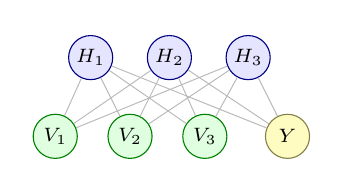
\begin{tikzpicture}[
  every node/.style={font=\scriptsize},
  unit/.style={circle, draw=gray!65, minimum size=0.56cm, inner sep=0pt},
  visible/.style={unit, fill=green!12, draw=green!50!black},
  labelunit/.style={unit, fill=yellow!24, draw=yellow!45!black},
  hidden/.style={unit, fill=blue!10, draw=blue!50!black},
  edge/.style={gray!55, line width=0.35pt}
]
  \path[use as bounding box] (-0.35,-0.38) rectangle (3.35,1.38);

  \node[visible] (v1) at (0.00,0) {$V_1$};
  \node[visible] (v2) at (0.95,0) {$V_2$};
  \node[visible] (v3) at (1.90,0) {$V_3$};
  \node[labelunit] (y) at (2.95,0) {$Y$};

  \node[hidden] (h1) at (0.45,1.00) {$H_1$};
  \node[hidden] (h2) at (1.45,1.00) {$H_2$};
  \node[hidden] (h3) at (2.45,1.00) {$H_3$};

  \foreach \v in {v1,v2,v3,y}
    \foreach \h in {h1,h2,h3}
      \draw[edge] (\v) -- (\h);
\end{tikzpicture}

\caption{RBM: \textcolor{blue!50!black}{$H_j$} connect only to visible features \textcolor{green!50!black}{$V_i$} and label \textcolor{yellow!45!black}{$Y$}; no within-layer edges.}
\label{fig:sl-restricted-boltzmann-machine-layers}
\end{figure}

\begin{remark} \label{rem:sl-separation-graphical-models} \hlt{Separation}\\
For disjoint vertex sets $A,B,C$, separation is a graphical certificate for $X_A\perp\!\!\!\perp X_B\mid X_C$: DAGs use d-separation, while undirected graphs use path separation by $C$.\\
Missing edges give pairwise certificates; separation gives setwise certificates.
\end{remark}

\subsection{Inference and Learning in Graphical Models}

Inference in a graphical model computes marginal, conditional, or most likely latent quantities from the joint law encoded by the graph.

\begin{definition} \label{def:sl-graphical-model-inference-tasks} \hlt{Inference Tasks}\\
Let $X=(X_j)_{j\in V}$ have joint law $p$, and let $A,B\subseteq V$ be disjoint. Standard \hlt{inference tasks} are:
\begin{enumerate}[label=(\roman*)]
\setlength{\itemsep}{0pt}
\item \hlt{Marginal inference}: compute $p(x_A)$.
\item \hlt{Conditional inference}: compute $p(x_A\mid x_B)$.
\item \hlt{MAP inference}: compute $x_A^\star\in\arg\max_{x_A}p(x_A\mid x_B)$, with $B=\varnothing$ for unconditional MAP.
\item \hlt{Latent posterior inference}: for latent $Z$ and observed $X=x$, compute $p(z\mid x)$.
\end{enumerate}
\end{definition}

\begin{method} \label{method:sl-message-passing} \hlt{Message Passing}\\
Let $G=(V,E)$ be a graphical model with local potentials.
\begin{enumerate}[label=(\roman*)]
\setlength{\itemsep}{0pt}
\item \hlt{Tree belief propagation}: on trees, two-way edge messages yield exact node and edge marginals.
\item \hlt{Loopy belief propagation}: on cyclic graphs, iterated message updates yield approximate marginals.
\end{enumerate}
\end{method}

\begin{definition} \label{def:sl-variational-inference} \hlt{Variational Inference}\\
For latent-variable model $p(x,z)$, intractable $p(z\mid x)$, tractable family $\mathcal{Q}$, \hlt{variational inference} choose $q^\star\in\mathcal{Q}$:
\begin{enumerate}[label=(\roman*)]
\setlength{\itemsep}{0pt}
\item \hlt{KL projection}: $q^\star\in\arg\min_{q\in\mathcal{Q}}\operatorname{KL}(q(z)\Vert p(z\mid x))$.
\item \hlt{ELBO maximization}: equivalently, maximize $\mathcal{L}(q)\defeq\mathbb{E}_q[\log p(x,z)]-\mathbb{E}_q[\log q(z)]$,\\
since $\log p(x)=\mathcal{L}(q)+\operatorname{KL}(q(z)\Vert p(z\mid x))$.
\end{enumerate}
\end{definition}

\begin{remark} \label{rem:sl-graphical-learning} \hlt{Learning Parameters and Structure}\\
Let $G$ denote the graph and $\theta$ its model parameters.
\begin{enumerate}[label=(\roman*)]
\setlength{\itemsep}{0pt}
\item \hlt{Parameter learning}: for fixed $G$, estimate $\theta$ by likelihood or regularized likelihood.
\item \hlt{Structure learning}: estimate unknown $G$ by optimizing a statistical score over graph candidates, often with structural penalties or combinatorial search.
\end{enumerate}
\end{remark}

\begin{method} \label{meth:sl-gaussian-graphical-model-learning} \hlt{Gaussian Graphical Model Learning}\\
For centered Gaussian data with empirical covariance $S$, let $\Theta=\Sigma^{-1}\succ0$ and $\ell(\Theta)\defeq\log\det\Theta-\operatorname{trace}(S\Theta)$.
\begin{enumerate}[label=(\roman*)]
\setlength{\itemsep}{0pt}
\item \hlt{Known graph}: for edge set $E$, estimate $\widehat{\Theta}\in\operatorname*{arg\,max}\limits_{\Theta\succ0}\ell(\Theta)$ subject to $\theta_{jk}=0$ whenever $\left\{j,k\right\}\notin E$.
\item \hlt{Unknown graph}: graphical lasso solves $\widehat{\Theta}\in\operatorname*{arg\,max}\limits_{\Theta\succ0}\left\{\ell(\Theta)-\lambda\sum\limits_{j\neq k}|\theta_{jk}|\right\}$, penalise off-diagonal entries.
\end{enumerate}
Graph selection is therefore shrinkage of inverse-covariance entries; zeros of $\widehat{\Theta}$ remove edges.
\end{method}

\begin{figure}[H]
\centering
\begin{tikzpicture}[
  >=Stealth,
  every node/.style={font=\scriptsize},
  vertex/.style={circle, draw=green!50!black, minimum size=0.56cm, inner sep=0pt, fill=green!12},
  sep/.style={circle, draw=orange!70!black, minimum size=0.56cm, inner sep=0pt, fill=orange!18},
  box/.style={draw=gray!65, rounded corners=2pt, minimum width=0.76cm, minimum height=0.42cm, inner sep=1.5pt, fill=gray!8},
  est/.style={box, draw=blue!55!black, fill=blue!8},
  flow/.style={-{Stealth[length=1.6mm]}, gray!70, line width=0.55pt},
  edge/.style={gray!65, line width=0.55pt}
]
  \path[use as bounding box] (-0.35,-0.45) rectangle (7.35,0.45);

  \node[vertex] (x) at (0.00,0) {$X$};
  \node[sep] (y) at (0.78,0) {$Y$};
  \node[vertex] (z) at (1.56,0) {$Z$};
  \node[vertex] (w) at (2.34,0) {$W$};
  \draw[edge] (x) -- (y);
  \draw[edge] (y) -- (z);
  \draw[edge] (z) -- (w);

  \node[box] (data) at (3.70,0) {$\mathcal D$};
  \node[box] (s) at (4.78,0) {$S$};
  \node[est] (theta) at (5.98,0) {$\widehat{\Theta}_\lambda$};
  \node[box] (graph) at (7.08,0) {$\widehat G$};

  \draw[flow] (data) -- (s);
  \draw[flow] (s) -- (theta);
  \draw[flow] (theta) -- (graph);
\end{tikzpicture}

\caption{$\mathcal D$ is the data and $S$ its empirical covariance. \textcolor{orange!70!black}{$Y$} gives $X\perp\{Z,W\}\mid Y$; graphical lasso solves $\widehat{\Theta}_\lambda\in\operatorname*{arg\,max}\limits_{\Theta\succ0}\left\{\log\det\Theta-\operatorname{tr}(S\Theta)-\lambda\sum_{j\ne k}|\theta_{jk}|\right\}$, and zeros of $\widehat{\Theta}_\lambda$ define missing edges in $\widehat G$.}
\label{fig:sl-markov-graph-separation-learning}
\end{figure}

\begin{breakablealgorithm}
\caption{Graphical Lasso by Block Coordinate Descent}
\label{alg:sl-graphical-lasso}
\begin{algorithmic}
\Require Empirical covariance $S\in\R^{p\times p}$, penalty $\lambda\geq0$
\Ensure Covariance estimate $W$ and sparse precision estimate $\widehat{\Theta}=W^{-1}$
\State Initialize $W\gets S+\lambda I$ and keep the diagonal fixed
\Repeat
\For{$j=1,\ldots,p$}
\State Partition $W$ into $W_{11}$, $w_{12}$, and $w_{22}$ by isolating  row and column $j$; partition $S$ similarly to get $s_{12}$
\State Define $\mathcal{S}_\lambda(z)=\sign(z)(|z|-\lambda)_+$
\Repeat
\For{$k=1,\ldots,p-1$}
\State $\displaystyle \beta_k\gets
\frac{\mathcal{S}_\lambda\!\left(s_{12,k}-\sum_{\ell\neq k}(W_{11})_{k\ell}\beta_\ell\right)}
{(W_{11})_{kk}}$
\EndFor
\Until{$\beta$ has converged for this block}
\State Update $w_{12}\gets W_{11}\beta$ and symmetrically update row and column $j$ of $W$
\EndFor
\Until{$W$ has converged}
\State In the final cycle recover $\widehat{\theta}_{12}=-\widehat{\beta}\widehat{\theta}_{22}$ with $1/\widehat{\theta}_{22}=w_{22}-w_{12}^T\widehat{\beta}$
\end{algorithmic} 
\end{breakablealgorithm}

\begin{method} \label{meth:sl-discrete-markov-network-learning} \hlt{Discrete Markov Network Learning}\\
For a binary Markov network with edge statistic $T_{jk}(X)=X_jX_k$, likelihood equations are $\widehat{\mathbb{E}}T_{jk}=\mathbb{E}_\Theta T_{jk}$ for $\{j,k\}\in E$; exact $\mathbb{E}_\Theta$ sums over $x\in\{0,1\}^p$.
\begin{enumerate}[label=(\roman*)]
\setlength{\itemsep}{0pt}
\item \hlt{Small graphs}: solve $\widehat{\mathbb{E}}T_{jk}=\mathbb{E}_\Theta T_{jk}$ by log-linear Poisson MLE, gradient/Newton updates,\\
or iterative proportional fitting.
\item \hlt{Large graphs}: approximate $\mathbb{E}_\Theta T_{jk}$ by mean-field or Gibbs-sampling estimates.
\item \hlt{Hidden-node models}: use observed-data conditionals for $\widehat{\mathbb{E}}T_{jk}$; for RBMs, CD-$r$ starts at data and\\
runs $r$ alternating Gibbs steps $h\sim p(h\mid v)$, $v\sim p(v\mid h)$.
\end{enumerate}
\end{method}

\subsection{Causal Graphs, Interventions, and Identifiability}

Causal learning asks which predictions remain valid under interventions, not merely under passive observation.

\begin{definition} \label{def:sl-structural-causal-model} \hlt{Structural Causal Model}\\
Let $J$ index endogenous variables $X=(X_j)_{j\in J}$ and exogenous disturbances $U=(U_j)_{j\in J}$.\\
A structural causal model is $M=(G,\{f_j\}_{j\in J},P_U)$ such that:
\begin{enumerate}[label=(\roman*)]
\setlength{\itemsep}{0pt}
\item $G=(J,E)$ is a directed graph with $\operatorname{pa}(j)=\{k\in J:k\to j\in E\}$.
\item $P_U$ is the joint law of $U$.
\item $X_j=f_j(X_{\operatorname{pa}(j)},U_j)$ for every $j\in J$.
\end{enumerate}
The edges $k\to j$ are the direct causal inputs to $X_j$.
\end{definition}

\begin{definition} \label{def:sl-intervention-do-operator} \hlt{Intervention}\\
For $M=(G,\{f_k\}_{k\in J},P_U)$ and $x\in\mathcal X_j$, set $\tilde f_j\equiv x$ and $\tilde f_k=f_k$ for $k\ne j$.\\
The \hlt{intervention} $\operatorname{do}(X_j=x)$ is the modified model $M_{j:=x}=(G_{j:=x},\{\tilde f_k\}_{k\in J},P_U)$, where $G_{j:=x}$ deletes all incoming edges to $j$; the induced law $P_{M_{j:=x}}$ is the interventional distribution.
\end{definition}

\begin{definition} \label{def:sl-causal-identifiability} \hlt{Identifiability}\\
Let $\mathcal M$ be the assumed model class and let $P_M$ be the observational law induced by $M\in\mathcal M$.\\
A causal functional $\psi:\mathcal M\to\Theta$ is \hlt{identifiable} on $\mathcal M$ if $P_M=P_{M'}$ implies $\psi(M)=\psi(M')$ for all $M,M'\in\mathcal M$.
\end{definition}

\begin{remark} \label{rem:sl-causal-versus-predictive} \hlt{Causal and Predictive Targets}\\
Let $\hat y=g(z)$ be trained under the observational law $P_M$. Small risk $R_{P_M}(g)=\mathbb E_{P_M}[\ell(Y,g(Z))]$ need not imply small interventional risk $R_{P_{M_{j:=x}}}(g)$ after $\operatorname{do}(X_j=x)$. Transport across regimes requires causal stability of the conditional mechanism used by $g$, not only predictive fit under $P_M$.
\end{remark}

\subsection{Counterfactuals and Policy Evaluation}

Policy learning and evaluation combine prediction with causal questions about actions not actually taken.

\begin{definition} \label{def:sl-potential-outcomes} \hlt{Potential Outcomes}\\
Let $A\in\mathcal A$ be a treatment.
\begin{enumerate}[label=(\roman*)]
\setlength{\itemsep}{0pt}
\item \hlt{Potential outcome}: $Y(a)$ is the outcome under $\operatorname{do}(A=a)$.
\item \hlt{Consistency}: $Y=Y(A)$.
\item \hlt{Individual effect}: for binary $A\in\{0,1\}$, $\tau=Y(1)-Y(0)$.
\item \hlt{Average treatment effect}: $\operatorname{ATE}=\mathbb E[\tau]$.
\end{enumerate}
\end{definition}

\begin{definition} \label{def:sl-ignorability-propensity} \hlt{Ignorability and Propensity}\\
For binary treatment $A$ and covariates $X$:
\begin{enumerate}[label=(\roman*)]
\setlength{\itemsep}{0pt}
\item \hlt{Ignorability}: $(Y(0),Y(1))\perp\!\!\!\perp A\mid X$.
\item \hlt{Propensity score}: $e(x)=P(A=1\mid X=x)$.
\item \hlt{Overlap}: $0<e(X)<1$ almost surely.
\end{enumerate}
\end{definition}

\begin{definition} \label{def:sl-off-policy-evaluation} \hlt{Off-Policy Evaluation}\\
Let $(X_i,A_i,Y_i)_{i=1}^n$ be logged under behavior policy $\mu(a\mid x)$, and let $\pi(a\mid x)$ be a target policy.
\begin{enumerate}[label=(\roman*)]
\setlength{\itemsep}{0pt}
\item \hlt{Target value}: $V(\pi)=\mathbb E_\pi[Y]$.
\item \hlt{Off-policy evaluation}: estimate $V(\pi)$ from data sampled under $\mu$.
\item \hlt{Inverse-propensity weighting}: $\hat V_{\operatorname{IPW}}(\pi)=n^{-1}\sum_{i=1}^n \{\pi(A_i\mid X_i)/\mu(A_i\mid X_i)\}Y_i$.
\item \hlt{Overlap}: $\mu(a\mid x)>0$ whenever $\pi(a\mid x)>0$.
\end{enumerate}
\end{definition}

\begin{remark} \label{rem:sl-feedback-policy-learning} \hlt{Feedback}\\
If a predictor $g$ induces actions through a policy $\pi_g(a\mid x)$, then future data are drawn from the post-deployment law $P^{\pi_g}$ rather than the pre-deployment law $P^0$. Feedback is the dependence $g\mapsto\pi_g\mapsto P^{\pi_g}$; causal learning, reinforcement learning, and deployment monitoring all study or control this induced law.
\end{remark}


\section{Neural Network Foundations}

\subsection{Network Architectures and Expressivity}

The migrated deep-feedforward-network notes describe neural networks as learned feature maps followed by prediction heads.

\begin{definition} \label{def:sl-feedforward-network} \hlt{Deep Feedforward Network}\\
Let $x\in\mathcal X$, set $h^{(0)}=x$, and fix depth $L$.
\begin{enumerate}[label=(\roman*)]
\setlength{\itemsep}{0pt}
\item \hlt{Layer recursion}: $h^{(k)}=g^{(k)}(W^{(k)}h^{(k-1)}+b^{(k)})$ for $k=1,\ldots,L$.
\item \hlt{Network map}: $f_\theta:\mathcal X\to\mathcal Y$ is $f_\theta(x)=h^{(L)}=(f_L\circ\cdots\circ f_1)(x)$.
\item \hlt{Parameters}: $\theta=\{(W^{(k)},b^{(k)})\}_{k=1}^L$.
\item \hlt{Training objective}: choose $\theta$ to minimize empirical risk $\hat R_n(f_\theta)$ or population risk $R(f_\theta)$.
\end{enumerate}
\end{definition}

\begin{remark} \label{rem:sl-learned-feature-map} \hlt{Learned Feature Maps}\\
Let $\ell$ be the task loss and let $R(f)=\mathbb E[\ell(Y,f(X))]$. Two representation parametrizations are:
\begin{enumerate}[label=(\roman*)]
\setlength{\itemsep}{0pt}
\item \hlt{fixed features}: $f_w(x)=a_w(\phi(x))$, with $\phi$ fixed and only the head parameter $w$ optimized.
\item \hlt{learned features}: $f_{\theta,w}(x)=a_w(\phi_\theta(x))$, with $\theta$ and $w$ optimized jointly.
\end{enumerate}
Learning $\phi_\theta$ adds adaptivity but usually destroys convexity.
\end{remark}

\begin{definition} \label{def:sl-projection-pursuit-ridge-functions} \hlt{Projection Pursuit and Ridge Functions}\\
Let $x\in\R^p$.
\begin{enumerate}[label=(\roman*)]
\setlength{\itemsep}{0pt}
\item \hlt{Projection-pursuit form}: $f(x)=\sum\limits_{m=1}^M g_m(\omega_m^Tx)$ with $\norm{\omega_m}_2=1$.
\item \hlt{Ridge coordinate}: $u_m=\omega_m^Tx$.
\item \hlt{Ridge function}: $g_m(u_m)$ depends on $x$ only through the scalar coordinate $u_m$.
\item \hlt{Learned components}: the directions $\omega_m$ and univariate profiles $g_m$ are estimated from data.
\end{enumerate}
\end{definition}

\begin{definition} \label{def:sl-output-and-hidden-units} \hlt{Output and Hidden Units}\\
Let $T\in\R^K$ denote output scores. Common output parametrizations are:
\begin{enumerate}[label=(\roman*)]
\setlength{\itemsep}{0pt}
\item \hlt{linear}: $f_k(x)=T_k$, for conditional means or real-valued responses.
\item \hlt{sigmoid}: $p(x)=\sigma(T)=\frac{1}{1+\exp(-T)}$, for Bernoulli probabilities.
\item \hlt{softmax}: $p_k(x)=\exp(T_k)/\sum\limits_{\ell=1}^K\exp(T_\ell)$, for $K$-class probabilities.
\end{enumerate}
Hidden units define activations $Z_m=\phi_m(a_m)$ from preactivations $a_m$, commonly using ReLU, leaky ReLU, maxout, $\tanh$, or another nonlinear map.
\end{definition}

\begin{definition} \label{def:sl-single-hidden-layer-network} \hlt{Single Hidden Layer Network}\\
Let $x\in\R^p$, $Z=(Z_1,\ldots,Z_M)^T$, $T=(T_1,\ldots,T_K)^T$. A single-hidden-layer feedforward network is defined by:
\begin{enumerate}[label=(\roman*)]
\setlength{\itemsep}{0pt}
\item $Z_m=\sigma(\alpha_{0m}+\alpha_m^Tx)$ for $m=1,\ldots,M$.
\item $T_k=\beta_{0k}+\beta_k^TZ$ for $k=1,\ldots,K$.
\item $f_k(x)=g_k(T)$, with $g_k(T)=T_k$ for regression and $g_k(T)=\exp(T_k)/\sum\limits_{\ell=1}^K\exp(T_\ell)$ for $K$-class classification.
\end{enumerate}
In the classification case, $f(x)\in\Delta^{K-1}$.
\end{definition}

\begin{figure}[H]
\centering
\begin{tikzpicture}[
    >=Stealth,
    font=\scriptsize,
    line cap=round,
    line join=round,
    block/.style={draw=gray!65, rounded corners=2pt, align=center,
        minimum height=0.72cm, inner xsep=6pt, inner ysep=2pt},
    input/.style={block, draw=cyan!65!black, fill=cyan!8, minimum width=1.65cm},
    hidden/.style={block, draw=blue!55!black, fill=blue!8, minimum width=2.85cm},
    score/.style={block, draw=orange!70!black, fill=orange!10, minimum width=2.65cm},
    flow/.style={->, draw=black!75, line width=0.6pt}
]
\node[input] (x) at (0,0) {inputs\\$x=(X_1,\ldots,X_p)$};
\path (x.east) ++(0.7,0) node[hidden, anchor=west] (z)
  {hidden features\\$Z_m=\sigma(\alpha_{0m}+\alpha_m^Tx)$};
\path (z.east) ++(0.7,0) node[score, anchor=west] (t)
  {output scores\\$T_k=\beta_{0k}+\beta_k^TZ$};

\draw[flow] (x) -- (z);
\draw[flow] (z) -- (t);
\end{tikzpicture}

\caption{Single-hidden-layer feedforward network.}
\label{fig:sl-single-hidden-layer-network}
\end{figure}

\begin{remark} \label{rem:sl-neural-networks-as-ridge-expansions} \hlt{Neural Networks as Ridge Expansions}\\
For scalar output, a one-hidden-layer network has $f(x)=\beta_0+\sum\limits_{m=1}^M\beta_m\sigma(\alpha_{0m}+\alpha_m^Tx)$.\\
If $\alpha_m\ne0$ and $\omega_m=\frac{\alpha_m}{\norm{\alpha_m}_2}$, the $m$th term is $\beta_m\sigma(\alpha_{0m}+\norm{\alpha_m}_2\omega_m^Tx)$, a ridge term in coordinate $\omega_m^Tx$ with learned \hlt{direction} $\omega_m$, \hlt{scale} $\norm{\alpha_m}_2$, \hlt{threshold} $\alpha_{0m}$, and \hlt{output coefficient} $\beta_m$.\\
Thus a shallow scalar network is a projection-pursuit expansion with parametrized ridge profiles.
\end{remark}

\begin{theorem} \label{thm:sl-universal-approximation-form} \hlt{Universal Approximation Theorem Form}\\
For compact $K\subset\R^d$, $h\in C(K)$, non-polynomial activation $\sigma:\R\to\R$, $\forall \varepsilon>0$, $\exists$ $M\in\mathbb{N}$, $a_m,b_m\in\R$, $w_m\in\R^d$ s.t. one-hidden-layer network $f_M(x)=\sum\limits_{m=1}^M a_m\sigma(w_m^\top x+b_m)$ satisfies $\norm{f_M-h}_\infty<\varepsilon$ on $K$.
\begin{proof} Let $\mathcal{A}_\sigma\defeq\operatorname{span}\{\sigma(w^\top x+b):w\in\R^d,\ b\in\R\}\subset C(K)$.\\
The classical universal approximation theorem states that $\overline{\mathcal{A}_\sigma}^{\norm{\cdot}_\infty}=C(K)$ for suitable non-polynomial $\sigma$.\\
Since $h\in C(K)$ and $\varepsilon>0$, there is $f_M\in\mathcal{A}_\sigma$ with $\norm{f_M-h}_\infty<\varepsilon$.\\
Thus $f_M(x)=\sum\limits_{m=1}^M a_m\sigma(w_m^\top x+b_m)$ has one hidden layer and linear output.\\
\hlt{Structural Commentary}: Non-polynomial activations make ridge spans dense in $C(K)$.\\
\hlt{Key Insight}: Width supplies finite linear combinations of nonlinear ridge functions.
\end{proof}
\end{theorem}

\begin{remark} \label{rem:sl-depth-expressivity} \hlt{Depth and Expressivity}\\
Let $N_L(\varepsilon,h)$ be the minimum width of a depth-$L$ network with $\norm{f-h}_\infty\le\varepsilon$ on a compact domain. Universal approximation gives $N_L(\varepsilon,h)<\infty$, not trainability; depth expressivity is $N_L(\varepsilon,h)\ll N_{L'}(\varepsilon,h)$ for some $L>L'$.
\end{remark}

\subsection{Backpropagation and Automatic Differentiation}

Backpropagation is reverse-mode differentiation applied to the computational graph of the network and loss.

\begin{definition} \label{def:sl-computational-graph} \hlt{Computational Graph}\\
A computational graph is a finite directed acyclic graph $G=(V,E)$ together with variables $(x_v)_{v\in V}$ and local maps $(f_v)_{v\in V\setminus S}$, where $\operatorname{pa}(v)=\{u\in V:(u,v)\in E\}$ and $S=\{v\in V:\operatorname{pa}(v)=\varnothing\}$.
\begin{enumerate}[label=(\roman*)]
\setlength{\itemsep}{0pt}
\item For $v\in S$, $x_v$ is an input, parameter, or constant.
\item For $v\in V\setminus S$, $x_v=f_v((x_u)_{u\in\operatorname{pa}(v)})$.
\item An edge $u\to v$ records the direct dependence of $x_v$ on $x_u$ in $f_v$.
\end{enumerate}
For scalar output $L=x_\ell$ and parameter sources $P\subseteq S$, reverse mode computes $(\partial L/\partial x_v)_{v\in V}$, hence $\nabla_{(x_p)_{p\in P}}L$.
\end{definition}

\begin{method} \label{method:sl-backpropagation} \hlt{Backpropagation}\\
Let $h^{(0)}=x$, $z^{(k)}=W^{(k)}h^{(k-1)}+b^{(k)}$, $h^{(k)}=\phi_k(z^{(k)})$ for $1\leq k\leq K$, and $L=\ell(h^{(K)},y)$.\\
Write $\bar u=\nabla_u L$ for the adjoint of $u$.
\begin{enumerate}[label=(\roman*)]
\setlength{\itemsep}{0pt}
\item Compute $z^{(k)}$ and $h^{(k)}$ for $k=1,\ldots,K$, then compute $L$.
\item Initialize $\bar h^{(K)}=\nabla_{h^{(K)}}\ell(h^{(K)},y)$.
\item For $k=K,\ldots,1$, set $\bar z^{(k)}=J_{\phi_k}(z^{(k)})^T\bar h^{(k)}$ and $(\nabla_{W^{(k)}}L,\nabla_{b^{(k)}}L,\bar h^{(k-1)})=(\bar z^{(k)}(h^{(k-1)})^T,\bar z^{(k)},(W^{(k)})^T\bar z^{(k)})$.
\end{enumerate}
Thus backpropagation is reverse-mode differentiation of $L$ through the layerwise computational graph.
\end{method}

\begin{method} \label{meth:sl-single-hidden-layer-backprop-equations} \hlt{Single-Hidden-Layer Backpropagation Equations}\\
For one training case $(x_i,y_i)$ in a single-hidden-layer network, let $m=1,\ldots,M$ index hidden units, $k=1,\ldots,K$ index output components, and $z_i=(z_{1i},\ldots,z_{Mi})^T$.
\begin{enumerate}[label=(\roman*)]
\setlength{\itemsep}{0pt}
\item Compute $a_{mi}=\alpha_{0m}+\alpha_m^Tx_i$, $z_{mi}=\sigma(a_{mi})$, $t_{ki}=\beta_{0k}+\beta_k^Tz_i$, and $f_k(x_i)=g_k(t_{ki})$.
\item Compute $R_i=\sum\limits_{k=1}^K\{y_{ik}-f_k(x_i)\}^2$ and $\delta_{ki}=\frac{\partial R_i}{\partial t_{ki}}=-2\{y_{ik}-f_k(x_i)\}g_k'(t_{ki})$.
\item Compute $\nabla_{\beta_k}R_i=\delta_{ki}z_i$ and $\frac{\partial R_i}{\partial\beta_{0k}}=\delta_{ki}$.
\item Compute $s_{mi}=\frac{\partial R_i}{\partial a_{mi}}=\sigma'(a_{mi})\sum\limits_{k=1}^K\beta_{km}\delta_{ki}$.
\item Compute $\nabla_{\alpha_m}R_i=s_{mi}x_i$ and $\frac{\partial R_i}{\partial\alpha_{0m}}=s_{mi}$.
\end{enumerate}
Batch gradients are obtained by summing these per-case derivatives over $i$.
\end{method}

\begin{breakablealgorithm}
\caption{Minibatch Backpropagation Step}
\begin{algorithmic}
\Require Minibatch $B$, parameters $\theta$, learning rate $\eta$
\State Compute predictions $f(x;\theta)$ for all $(x,y)\in B$
\State Compute minibatch loss $\widehat{L}_B(\theta)$
\State Run reverse-mode automatic differentiation to compute $g=\nabla_{\theta}\widehat{L}_B(\theta)$
\State Update parameters $\theta \leftarrow \theta-\eta g$
\end{algorithmic}
\end{breakablealgorithm}

\begin{remark} \label{rem:sl-autodiff-versus-symbolic} \hlt{Automatic Differentiation}\\
For an implemented graph map $F:\mathbb{R}^p\to\mathbb{R}^q$, automatic differentiation returns $DF(x)$ by chain-rule evaluation on the executed graph.  It differentiates the floating-point computation up to roundoff, without finite differences or symbolic simplification.
\end{remark}

\subsection{Optimization for Deep Learning}

The old optimization notes are migrated here only where the algorithms are used as training methods for neural networks.  General numerical optimization belongs to Part 14.

\begin{definition} \label{def:sl-neural-empirical-objective} \hlt{Neural Empirical Objective}\\
For data $(x_i,y_i)_{i=1}^n$, network $f_\theta:x\mapsto f(x;\theta)$, loss $L$, neural empirical objective is $J_n(\theta)=n^{-1}\sum\limits_{i=1}^nL(f_\theta(x_i),y_i)$.\\
The population objective is $J(\theta)=\mathbb E[L(f_\theta(X),Y)]$ under the data-generating law.
\end{definition}

\begin{breakablealgorithm}
\caption{Minibatch Backpropagation Step}
\begin{algorithmic}
\Require Minibatch $B$, parameters $\theta$, learning rate $\eta$
\State Compute predictions $f(x;\theta)$ for all $(x,y)\in B$
\State Compute minibatch loss $\widehat{L}_B(\theta)$
\State Run reverse-mode automatic differentiation to compute $g=\nabla_{\theta}\widehat{L}_B(\theta)$
\State Update parameters $\theta \leftarrow \theta-\eta g$
\end{algorithmic}
\end{breakablealgorithm}

\begin{remark} \label{rem:sl-deep-optimization-challenges} \hlt{Deep Optimization Challenges}\\
For empirical loss $J_n(\theta)$, deep optimization is shaped by:
\begin{enumerate}[label=(\roman*)]
\setlength{\itemsep}{0pt}
\item \hlt{geometry}: large $\kappa(\nabla^2J_n)$, saddles with $\nabla J_n\approx0$ and indefinite $\nabla^2J_n$, and plateaus with $\norm{\nabla J_n}\approx0$.
\item \hlt{gradient propagation}: large or small $\norm{\frac{\partial h^{(L)}}{\partial h^{(k)}}}$ causes exploding or vanishing gradients.
\item \hlt{stochasticity}: $g_k=\nabla J_n(\theta_k)+\xi_k$, with $\mathbb E[\xi_k\mid\theta_k]=0$ and $\operatorname{Var}(\xi_k\mid\theta_k)\ne0$.
\item \hlt{stabilization}: initialization, normalization, gradient clipping, skip connections, and learning-rate schedules control scale, conditioning, and update variance.
\end{enumerate}
These choices are part of the training specification, not post hoc implementation details.
\end{remark}

\subsection{Regularization, Normalization, and Generalization}

Deep-learning regularization combines penalties, stochastic training effects, architecture, and validation-based stopping.

\begin{definition} \label{def:sl-neural-regularized-objective} \hlt{Parameter-Norm Regularization}\\
Minimize $\widetilde J_\lambda(\theta)=J(\theta)+\lambda\Omega(\theta)$, with $\lambda\geq0$, $\Omega\geq0$, and penalized non-intercept set $\mathcal P$.
\begin{enumerate}[label=(\roman*)]
\setlength{\itemsep}{0pt}
\item \hlt{$\ell^2$ weight decay}: $\Omega_2(\theta)=\sum\limits_{j\in\mathcal P}\theta_j^2$.
\item \hlt{$\ell^1$ penalty}: $\Omega_1(\theta)=\sum\limits_{j\in\mathcal P}\abs{\theta_j}$.
\item \hlt{Single-hidden-layer weight decay}: for weights $\alpha_{m\ell}$ and $\beta_{km}$, $\Omega_2(\theta)=\sum\limits_{m,\ell}\alpha_{m\ell}^2+\sum\limits_{k,m}\beta_{km}^2$.
\end{enumerate}
Intercepts such as $\alpha_{0m}$ and $\beta_{0k}$ are excluded unless explicitly included in $\mathcal P$.
\end{definition}

\begin{definition} \label{def:sl-dropout} \hlt{Dropout}\\
Let $h\in\R^d$, $q\in(0,1]$, and $m_j\overset{\mathrm{ind}}{\sim}\operatorname{Bernoulli}(q)$.
\begin{enumerate}[label=(\roman*)]
\setlength{\itemsep}{0pt}
\item \hlt{Training mask}: replace $h$ by $\widetilde h=\frac{m\odot h}{q}$.
\item \hlt{Subnetwork}: each mask $m\in\{0,1\}^d$ selects the active coordinates $\{j:m_j=1\}$ with shared parameters.
\item \hlt{Evaluation}: use the unmasked activation $h$ when inverted dropout scaling is used in training.
\end{enumerate}
Dropout optimizes an expected masked loss over tied-parameter subnetworks.
\end{definition}

\begin{method} \label{method:sl-early-stopping} \hlt{Early Stopping}\\
Let $\theta_t$ be the parameter after training step $t$ and let $V(\theta)$ be the validation loss.
\begin{enumerate}[label=(\roman*)]
\setlength{\itemsep}{0pt}
\item Compute $V_t=V(\theta_t)$ after selected training steps $t$.
\item Select $t^\star\in\operatorname*{arg\,min}_{0\leq t\leq T}V_t$.
\item Return $\widehat\theta_{\mathrm{ES}}=\theta_{t^\star}$.
\end{enumerate}
The stopping time $t^\star$ restricts the reachable parameter set and acts as an implicit regularization parameter.
\end{method}

\begin{remark} \label{rem:sl-neural-training-practicalities} \hlt{Starting Values, Scaling, and Multiple Fits}\\
For a nonconvex neural objective $J(\theta)$, the fitted parameter can depend on initialization and scaling.
\begin{enumerate}[label=(\roman*)]
\setlength{\itemsep}{0pt}
\item \hlt{Initialization}: avoid $\theta_0=0$ when symmetry identifies hidden units, and avoid large $\norm{\theta_0}$ when $\sigma'(a)\approx0$.
\item \hlt{Scaling}: standardize inputs, e.g. $x_j\leftarrow\frac{x_j-\hat\mu_j}{\hat\sigma_j}$, so coordinates have comparable optimization scale.
\item \hlt{Multiple fits}: run starts $r=1,\ldots,R$, obtain $\widehat\theta^{(r)}$, and choose $\widehat\theta^{(r^\star)}$ by validation or penalized criterion.
\end{enumerate}
Thus initialization law, preprocessing, and restart selection are part of the training specification.
\end{remark}

\begin{remark} \label{rem:sl-hidden-units-and-weight-decay} \hlt{Hidden Units and Weight Decay}\\
Let $M$ be hidden width, $\lambda$ the weight-decay strength, and $t^\star$ the early-stopping time.
\begin{enumerate}[label=(\roman*)]
\setlength{\itemsep}{0pt}
\item \hlt{Small $M$}: the model class may have excessive approximation error.
\item \hlt{Large $M$}: overfitting can occur unless $\lambda>0$, finite $t^\star$, or another constraint limits effective complexity.
\item \hlt{Selection}: choose $(M,\lambda,t^\star)$ by validation or another held-out criterion.
\end{enumerate}
Weight decay and early stopping bias the fit toward smaller effective weights and simpler functions.
\end{remark}

\begin{definition} \label{def:sl-batch-normalization} \hlt{Batch Normalization}\\
Let $H=(h_{ij})\in\R^{b\times d}$ be minibatch activations, indexed by example $i$ and coordinate $j$.
\begin{enumerate}[label=(\roman*)]
\setlength{\itemsep}{0pt}
\item \hlt{Batch statistics}: $\mu_j=\frac{1}{b}\sum\limits_i h_{ij}$ and $s_j^2=\frac{1}{b}\sum\limits_i(h_{ij}-\mu_j)^2$.
\item \hlt{Normalization}: $\widehat h_{ij}=\frac{h_{ij}-\mu_j}{\sqrt{s_j^2+\varepsilon}}$.
\item \hlt{Affine output}: $y_{ij}=\gamma_j\widehat h_{ij}+\beta_j$, with learned $\gamma_j,\beta_j$.
\item \hlt{Evaluation}: replace $\mu_j$ and $s_j^2$ by running training estimates.
\end{enumerate}
\end{definition}

\begin{remark} \label{rem:sl-data-augmentation-noise} \hlt{Augmentation and Noise}\\
Let $\ell(y,f_\theta(x))$ be the task loss.
\begin{enumerate}[label=(\roman*)]
\setlength{\itemsep}{0pt}
\item \hlt{Data augmentation}: replace $(X,Y)$ by $(T(X),Y)$ for random label-preserving transforms $T$.
\item \hlt{Label smoothing}: replace one-hot $y$ by $y^{(\varepsilon)}=(1-\varepsilon)y+\varepsilon u$, where $u$ is a reference class distribution.
\item \hlt{Noise injection}: train on $x+\xi$ or hidden activations $h+\xi$, with $\mathbb E\xi=0$.
\item \hlt{Adversarial training}: minimize $\ell(y,f_\theta(x+\delta^\star))$, where $\delta^\star\in\operatorname*{arg\,max}\limits_{\norm{\delta}\leq\rho}\ell(y,f_\theta(x+\delta))$.
\item \hlt{Multitask learning}: minimize $\sum\limits_{r=1}^R\omega_r\ell_r(y_r,f_{\theta,r}(x))$ with shared representation parameters.
\end{enumerate}
These methods regularize through altered data, targets, perturbations, or shared representations.
\end{remark}


\section{Modern Deep Models}

\subsection{Convolutional and Geometric Architectures}

The convolutional-network source is migrated here because convolution is an architectural prior for data with grid, group, or geometric structure.

\begin{definition} \label{def:sl-convolution} \hlt{Convolution}\\
For $f,g:\R\to\R$ and $a,b:\Z\to\R$:
\begin{enumerate}[label=(\roman*)]
\setlength{\itemsep}{0pt}
\item \hlt{Continuous}: $f*g:D_c\ni t\mapsto\int_{-\infty}^{\infty}f(\tau)g(t-\tau)\,d\tau\in\R$; $D_c\defeq\{t\in\R:\int_\R\abs{f(\tau)g(t-\tau)}\,d\tau<\infty\}$.
\item \hlt{Discrete}: $a*b:D_d\ni n\mapsto\sum\limits_{m\in\Z}a[m]b[n-m]\in\R$; $D_d\defeq\{n\in\Z:\sum\limits_{m\in\Z}\abs{a[m]b[n-m]}<\infty\}$.
\end{enumerate}
\end{definition}

\begin{definition} \label{def:sl-convolutional-neural-network} \hlt{Convolutional Neural Network}\\
Let $\Phi=L_k\circ\cdots\circ L_1$ be a neural network on array-valued activations.
\begin{enumerate}[label=(\roman*)]
\setlength{\itemsep}{0pt}
\item \hlt{Convolutional layer}: on $z:\Z^d\to\R^{C_{\rm in}}$, $L_jz=\sigma(K*z+b)$ or $\sigma(K\star z+b)$, with finite-support $K$, $b\in\R^{C_{\rm out}}$, pointwise $\sigma$, and cross-correlation $\star$.
\item \hlt{Convolutional neural network}: $\Phi$ is a CNN if at least one layer $L_j$ is convolutional.
\item \hlt{Library convention}: many neural-network libraries implement $\star$ while naming the operation convolution.
\end{enumerate}
\end{definition}

\begin{definition} \label{def:sl-sparse-sharing-equivariance} \hlt{Sparse Interactions, Sharing, and Equivariance}\\
For $x:\Z^d\to\R^{C_{\rm in}}$, finite $W\subset\Z^d$, kernels $K_w\in\R^{C_{\rm out}\times C_{\rm in}}$, $b\in\R^{C_{\rm out}}$, and pointwise $\sigma$,\\
set $Lx(u)\defeq\sigma(\sum\limits_{w\in W}K_wx(u-w)+b)$ and $(\tau_a x)(u)\defeq x(u-a)$.
\begin{enumerate}[label=(\roman*)]
\setlength{\itemsep}{0pt}
\item \hlt{Sparse interaction}: $Lx(u)$ depends only on $\{x(u-w):w\in W\}$.
\item \hlt{Parameter sharing}: the same $(K_w)_{w\in W}$ and $b$ define $Lx(u)$ for every $u$.
\item \hlt{Translation equivariance}: $L(\tau_a x)=\tau_a(Lx)$ for every $a\in\Z^d$ where defined.
\end{enumerate}
Pooling with finite $U$ applies $\rho$ to $\{Lx(u+w):w\in U\}$; shift-stable $\rho$ gives local approximate invariance.
\end{definition}

\begin{definition} \label{def:sl-pooling-padding-stride} \hlt{Pooling, Padding, and Stride}\\
Let $x:\Omega\to\R^C$ on finite $\Omega\subset\Z^d$, with $W\subset\Z^d$, $p\in\N_0^d$, $s\in\N^d$, offset $r$, statistic $\rho:(\R^C)^W\to\R^{C'}$,\\
and $\Omega^{(p)}\defeq\Omega+\prod\limits_i\{-p_i,\ldots,p_i\}$.
\begin{enumerate}[label=(\roman*)]
\setlength{\itemsep}{0pt}
\item \hlt{Padding}: an extension $\tilde x:\Omega^{(p)}\to\R^C$ with $\tilde x|_{\Omega}=x$ and a boundary rule on $\Omega^{(p)}\setminus\Omega$.
\item \hlt{Stride}: evaluation sites $\Omega_{s,r}\defeq\{u\in\Omega^{(p)}:\forall i,\ u_i\equiv r_i\pmod{s_i},\ u+W\subset\Omega^{(p)}\}$.
\item \hlt{Pooling}: $P_{\rho,W,s,r}x:\Omega_{s,r}\ni u\mapsto\rho((\tilde x(u+w))_{w\in W})\in\R^{C'}$.
\end{enumerate}
\end{definition}

\begin{remark} \label{rem:sl-geometric-deep-learning} \hlt{Geometric Extensions}\\
Let $X$ be a domain with local neighborhoods $\mathcal N(x)\subset X$ and symmetry group $G$.
\begin{enumerate}[label=(\roman*)]
\setlength{\itemsep}{0pt}
\item \hlt{Graph neural networks}: on $\mathcal G=(V,E)$, $h_v^{(\ell+1)}=\phi(h_v^{(\ell)},\operatorname{Agg}\limits_{u\in\mathcal N(v)}m_{uv}^{(\ell)})$ with invariant $\operatorname{Agg}$.
\item \hlt{Equivariant networks}: $\Phi$ is $G$-equivariant if $\Phi(\rho_{\rm in}(g)x)=\rho_{\rm out}(g)\Phi(x)$ for every $g\in G$.
\item \hlt{Manifold architectures}: for a manifold $M$, layers use chart, tangent, or geodesic neighborhoods $\mathcal N(p)\subset M$.
\end{enumerate}
Each variant builds locality or symmetry into the model class.
\end{remark}

\subsection{Sequence Models and Attention}

Sequence models process ordered data where context and position matter.

\begin{definition} \label{def:sl-recurrent-network} \hlt{Recurrent Neural Network}\\
For dim $d_x,d_h,d_y$, parameters $\Theta=(W_x,W_h,b,\phi,\psi,h_0)$, $T\geq1$, an RNN is a map $\Phi_T:(\R^{d_x})^T\to(\R^{d_y})^T$:
\begin{enumerate}[label=(\roman*)]
\setlength{\itemsep}{0pt}
\item \hlt{State update}: $h_t=\phi(W_xx_t+W_hh_{t-1}+b)$ for $t=1,\ldots,T$, with shared $(W_x,W_h,b)$.
\item \hlt{Readout}: $y_t=\psi(h_t)$ and $\Phi_T(x_{1:T})=(y_1,\ldots,y_T)$.
\end{enumerate}
\end{definition}

\begin{remark} \label{rem:sl-long-term-dependencies} \hlt{Long-Term Dependencies}\\
For $h_t=F_t(h_{t-1},x_t)$, set $J_t\defeq\partial h_t/\partial h_{t-1}$ and $P_{s:T}\defeq\prod\limits_{t=s+1}^T J_t$.\\
Then $\nabla_{h_s}\mathcal L=P_{s:T}^\top\nabla_{h_T}\mathcal L$; $\norm{P_{s:T}}\ll1$ vanishes gradients and $\norm{P_{s:T}}\gg1$ explodes them.
\begin{enumerate}[label=(\roman*)]
\setlength{\itemsep}{0pt}
\item \hlt{Gating}: gates $g_t\in[0,1]^{d_h}$ interpolate between copy and update.
\item \hlt{Gradient clipping}: replace a gradient $g$ by $\min\{1,c/\norm g\}g$, so the clipped norm is at most $c$.
\item \hlt{Skip paths}: use additive routes such as $h_t=h_{t-1}+F_t(h_{t-1},x_t)$, giving transition Jacobian $I+\partial F_t/\partial h_{t-1}$.
\end{enumerate}
These mechanisms keep the long-horizon Jacobian product numerically controlled.
\end{remark}

\begin{definition} \label{def:sl-attention} \hlt{Attention}\\
For $Q\in\R^{n_q\times d}$, $K\in\R^{n_k\times d}$, $V\in\R^{n_k\times d_v}$, define $\operatorname{Attn}(Q,K,V)\in\R^{n_q\times d_v}$ row-wise:
\begin{enumerate}[label=(\roman*)]
\setlength{\itemsep}{0pt}
\item \hlt{Scores}: $S\defeq d^{-1/2}QK^\top\in\R^{n_q\times n_k}$.
\item \hlt{Weights}: $A\defeq\operatorname{softmax}_{\rm row}(S)$, $A_{ij}\defeq\exp(S_{ij})/\sum_{\ell=1}^{n_k}\exp(S_{i\ell})$.
\item \hlt{Output}: $\operatorname{Attn}(Q,K,V)\defeq AV$, equivalently $(\operatorname{Attn}(Q,K,V))_{i\cdot}=\sum_{j=1}^{n_k}A_{ij}V_{j\cdot}$.
\end{enumerate}
\end{definition}

\begin{remark} \label{rem:sl-attention-as-routing} \hlt{Attention as Routing}\\
For token matrix $X$, set $Q=XW_q$, $K=XW_k$, $V=XW_v$, $S=d^{-1/2}QK^\top$, and $A=\operatorname{softmax}_{\rm row}(S)$.
\begin{enumerate}[label=(\roman*)]
\setlength{\itemsep}{0pt}
\item \hlt{Content routing}: $y_i=\sum_j A_{ij}v_j$ routes value vectors by query-key compatibility.
\item \hlt{Masking}: a mask $M_{ij}\in\{0,-\infty\}$ replaces $S$ by $S+M$, forcing $A_{ij}=0$ for forbidden interactions.
\item \hlt{Positional encoding}: absolute codes use $x_i+e_i$; relative codes add a position term to $S_{ij}$.
\end{enumerate}
Thus attention replaces a fixed recurrence neighborhood by data-dependent communication.
\end{remark}

\subsection{Transformers and Large-Scale Training}

Transformers combine attention, feedforward blocks, normalization, and residual connections into architectures that scale well on sequence and multimodal data.

\begin{definition} \label{def:sl-transformer-block} \hlt{Transformer Block}\\
A transformer block applies multi-head self-attention, residual connections, normalization layers, and a positionwise feedforward network.  Stacking these blocks yields deep contextual representations.
\end{definition}

\begin{definition} \label{def:sl-self-attention} \hlt{Self-Attention}\\
Self-attention uses the same sequence to form queries, keys, and values.  Multi-head attention runs several attention maps in parallel and recombines their outputs.
\end{definition}

\begin{remark} \label{rem:sl-large-scale-training} \hlt{Large-Scale Training}\\
Large-scale deep learning is constrained by optimization, data quality, memory, communication, and evaluation.  Batch size, learning-rate schedules, mixed precision, parallelism, and checkpointing are part of the mathematical and systems design of training.
\end{remark}

\begin{remark} \label{rem:sl-transformer-generalization} \hlt{Inductive Bias}\\
Transformers have weaker built-in locality bias than convolutional networks but stronger capacity for long-range interaction.  Domain-specific variants add locality, recurrence, sparsity, or equivariance when the task demands it.
\end{remark}

\subsection{Generative Models}

Generative modeling learns distributions, simulators, or conditional samplers rather than only point predictions.

\begin{definition} \label{def:sl-latent-variable-generative-model} \hlt{Latent-Variable Generative Model}\\
Let $Z\in\mathcal Z$, $X\in\mathcal X$, prior $p(z)$, decoder $p_\theta(x\mid z)$, and data law $P_{\rm data}$.
\begin{enumerate}[label=(\roman*)]
\setlength{\itemsep}{0pt}
\item \hlt{Joint law}: $p_\theta(x,z)\defeq p_\theta(x\mid z)p(z)$.
\item \hlt{Marginal law}: $p_\theta(x)\defeq\int_{\mathcal Z}p_\theta(x\mid z)p(z)\,dz$.
\item \hlt{Learning}: choose $\theta$ so $p_\theta$ approximates $P_{\rm data}$, e.g. by maximizing $\sum_{i=1}^n\log p_\theta(x_i)$.
\end{enumerate}
\end{definition}

\begin{definition} \label{def:sl-variational-autoencoder} \hlt{Variational Autoencoder}\\
For prior $p(z)$, decoder $p_\theta(x\mid z)$, encoder $q_\phi(z\mid x)$, and data $\{x_i\}_{i=1}^n$:
\begin{enumerate}[label=(\roman*)]
\setlength{\itemsep}{0pt}
\item \hlt{Generative model}: $p_\theta(x,z)\defeq p_\theta(x\mid z)p(z)$.
\item \hlt{Variational posterior}: $q_\phi(z\mid x)$ approximates $p_\theta(z\mid x)$.
\item \hlt{ELBO}: $\mathcal L(\theta,\phi;x)\defeq\mathbb{E}_{q_\phi(z\mid x)}[\log p_\theta(x\mid z)]-\operatorname{KL}(q_\phi(z\mid x)\|p(z))$.
\item \hlt{Training}: maximize $\sum_{i=1}^n\mathcal L(\theta,\phi;x_i)$ over $(\theta,\phi)$.
\end{enumerate}
\end{definition}

\begin{definition} \label{def:sl-generative-adversarial-network} \hlt{Generative Adversarial Network}\\
Let $Z\sim p_Z$, data law $P_{\rm data}$, generator $G_\theta:\mathcal Z\to\mathcal X$, and discriminator $D_\psi:\mathcal X\to(0,1)$.
\begin{enumerate}[label=(\roman*)]
\setlength{\itemsep}{0pt}
\item \hlt{Generator}: $G_\theta$ induces $P_\theta\defeq(G_\theta)_\#p_Z$ on $\mathcal X$.
\item \hlt{Discriminator}: $D_\psi(x)$ estimates the probability that $x\sim P_{\rm data}$ rather than $x\sim P_\theta$.
\item \hlt{Adversarial game}: $\min_\theta\max_\psi\mathbb{E}_{x\sim P_{\rm data}}\log D_\psi(x)+\mathbb{E}_{z\sim p_Z}\log(1-D_\psi(G_\theta(z)))$.
\end{enumerate}
\end{definition}

\begin{definition} \label{def:sl-diffusion-model} \hlt{Diffusion Model}\\
Let $X_0\sim P_{\rm data}$ and $X_0,\ldots,X_T$ be a Markov chain on $\mathcal X$.
\begin{enumerate}[label=(\roman*)]
\setlength{\itemsep}{0pt}
\item \hlt{Forward noising}: fixed kernels $q_t(x_t\mid x_{t-1})$ define $q(x_{1:T}\mid x_0)=\prod_{t=1}^Tq_t(x_t\mid x_{t-1})$.
\item \hlt{Reverse model}: learned kernels $p_\theta(x_{t-1}\mid x_t)$ define $p_\theta(x_{0:T})=p_T(x_T)\prod_{t=1}^Tp_\theta(x_{t-1}\mid x_t)$.
\item \hlt{Training}: fit $\theta$ so $p_\theta(x_{t-1}\mid x_t)$ approximates the reverse conditionals of $q$.
\item \hlt{Sampling}: draw $X_T\sim p_T$ and iterate $X_{t-1}\sim p_\theta(\cdot\mid X_t)$ for $t=T,\ldots,1$.
\end{enumerate}
\end{definition}

\subsection{Reinforcement Learning and Decision Systems}

Reinforcement learning studies agents whose actions affect future observations and rewards.

\begin{definition} \label{def:sl-markov-decision-process} \hlt{Markov Decision Process}\\
An MDP is a tuple $(\mathcal S,\mathcal A,P,r,\gamma)$ with:
\begin{enumerate}[label=(\roman*)]
\setlength{\itemsep}{0pt}
\item \hlt{State-action spaces}: states $s\in\mathcal S$ and actions $a\in\mathcal A$.
\item \hlt{Transition law}: $P(\cdot\mid s,a)\in\mathcal P(\mathcal S)$ and $S_{t+1}\sim P(\cdot\mid S_t,A_t)$.
\item \hlt{Reward and discount}: $r:\mathcal S\times\mathcal A\to\R$ and $\gamma\in[0,1)$.
\item \hlt{Policy}: $\pi(\cdot\mid s)\in\mathcal P(\mathcal A)$ and $A_t\sim\pi(\cdot\mid S_t)$.
\end{enumerate}
\end{definition}

\begin{definition} \label{def:sl-value-functions} \hlt{Value Functions}\\
For policy $\pi$, define the discounted return $G_t\defeq\sum\limits_{k=0}^{\infty}\gamma^kr(S_{t+k},A_{t+k})$.
\begin{enumerate}[label=(\roman*)]
\setlength{\itemsep}{0pt}
\item \hlt{State value}: $V^\pi(s)\defeq\mathbb{E}_\pi[G_0\mid S_0=s]$.
\item \hlt{Action value}: $Q^\pi(s,a)\defeq\mathbb{E}_\pi[G_0\mid S_0=s,A_0=a]$.
\end{enumerate}
\end{definition}

\begin{definition} \label{def:sl-bellman-equation} \hlt{Bellman Equation}\\
For an MDP $(\mathcal S,\mathcal A,P,r,\gamma)$ and value function $V:\mathcal S\to\R$:
\begin{enumerate}[label=(\roman*)]
\setlength{\itemsep}{0pt}
\item \hlt{Policy Bellman equation}: $V^\pi(s)=\sum_a\pi(a\mid s)(r(s,a)+\gamma\sum_{s'}P(s'\mid s,a)V^\pi(s'))$.
\item \hlt{Optimal Bellman equation}: $V^\star(s)=\max_a(r(s,a)+\gamma\sum_{s'}P(s'\mid s,a)V^\star(s'))$.
\end{enumerate}
\end{definition}

\begin{remark} \label{rem:sl-rl-learning-systems} \hlt{RL as a Learning System}\\
Let $\tau=(S_0,A_0,R_0,\ldots)$ denote a trajectory and $P^\pi$ its law under policy $\pi$.
\begin{enumerate}[label=(\roman*)]
\setlength{\itemsep}{0pt}
\item \hlt{Prediction}: estimate $V^\pi$, $Q^\pi$, or transition/reward models from trajectories.
\item \hlt{Feedback}: policy changes alter the data law, $\pi\mapsto P^\pi$.
\item \hlt{Optimization}: choose $\pi$ to maximize $J(\pi)\defeq\mathbb{E}_{P^\pi}\sum\limits_{t\geq0}\gamma^tR_t$.
\item \hlt{Exploration}: sample actions to reduce uncertainty about rewards, transitions, or values.
\item \hlt{Evaluation}: validate under sequential dependence and policy-induced distribution shift.
\end{enumerate}
\end{remark}


\section{Learning Systems and Evaluation}

\subsection{Data Splitting, Validation, and Benchmarking}

Evaluation estimates how the trained system behaves on data not used to fit it.

\begin{definition} \label{def:sl-train-validation-test} \hlt{Training, Validation, and Test Splits}\\
Let $\mathcal{D}=\mathcal{D}_{\mathrm{tr}}\dot\cup\mathcal{D}_{\mathrm{val}}\dot\cup\mathcal{D}_{\mathrm{te}}$ be a disjoint partition of $\{(x_i,y_i)\}_{i=1}^n$, and fix a loss $\ell$.
\begin{enumerate}[label=(\roman*)]
\setlength{\itemsep}{0pt}
\item Training: for each $\lambda\in\Lambda$, fit $\widehat f_\lambda$ using only $\mathcal{D}_{\mathrm{tr}}$.
\item Validation: set $\widehat\lambda\in\arg\min_{\lambda\in\Lambda}\widehat R_{\mathrm{val}}(\lambda)$, where $\widehat R_{\mathrm{val}}(\lambda)=|\mathcal{D}_{\mathrm{val}}|^{-1}\sum_{(x,y)\in\mathcal{D}_{\mathrm{val}}}\ell(\widehat f_\lambda(x),y)$.
\item Test: after $\widehat\lambda$ is fixed, report $\widehat R_{\mathrm{te}}=|\mathcal{D}_{\mathrm{te}}|^{-1}\sum_{(x,y)\in\mathcal{D}_{\mathrm{te}}}\ell(\widehat f_{\widehat\lambda}(x),y)$ as the final performance estimate.
\end{enumerate}
If $\mathcal{D}_{\mathrm{val}}$ is unavailable, cross-validation or bootstrap resampling approximates validation.\\
Any pre-reporting use of $\mathcal{D}_{\mathrm{te}}$ makes $\widehat R_{\mathrm{te}}$ adaptive and typically optimistic.
\end{definition}

\begin{figure}[H]
  \centering
  \begin{tikzpicture}[
  >=Stealth,
  font=\scriptsize,
  line cap=round,
  line join=round,
  block/.style={draw=gray!65, rounded corners=2pt, minimum height=0.76cm,
    anchor=west, align=center, inner xsep=5pt, inner ysep=2pt},
  train/.style={block, draw=cyan!65!black, fill=cyan!8, minimum width=3.1cm},
  valid/.style={block, draw=green!45!black, fill=green!8, minimum width=2.35cm},
  test/.style={block, draw=orange!70!black, fill=orange!10, minimum width=2.2cm},
  tick/.style={draw=black!45, line width=0.45pt}
]
  \node[train] (train) at (0,0) {$\mathcal D_{\mathrm{tr}}$\\fit $\widehat{f}_\lambda$};
  \node[valid] (valid) at (3.1,0) {$\mathcal D_{\mathrm{val}}$\\select $\widehat{\lambda}$};
  \node[test] (test) at (5.45,0) {$\mathcal D_{\mathrm{te}}$\\report $\widehat{R}_{\mathrm{te}}$};

  \draw[tick] (0,-0.52) -- (7.65,-0.52);
  \draw[tick] (0,-0.42) -- (0,-0.62) node[below] {$0$};
  \draw[tick] (3.1,-0.42) -- (3.1,-0.62) node[below] {$n_{\mathrm{tr}}$};
  \draw[tick] (5.45,-0.42) -- (5.45,-0.62) node[below] {$n_{\mathrm{tr}}+n_{\mathrm{val}}$};
  \draw[tick] (7.65,-0.42) -- (7.65,-0.62) node[below] {$n$};
\end{tikzpicture}

  \caption[Train/validation/test split]{Train/validation/test split: $\mathcal D=\mathcal D_{\mathrm{tr}}\sqcup\mathcal D_{\mathrm{val}}\sqcup\mathcal D_{\mathrm{te}}$, with $\mathcal D_{\mathrm{tr}}$ fitting $\widehat{f}_\lambda$, $\mathcal D_{\mathrm{val}}$ selecting $\widehat{\lambda}$, and $\mathcal D_{\mathrm{te}}$ estimating final risk $\widehat{R}_{\mathrm{te}}$.}
  \label{fig:sl-train-validation-test-split}
\end{figure}

\begin{definition} \label{def:sl-model-selection-versus-assessment} \hlt{Model Selection and Model Assessment}\\
Let $\{\widehat f_\lambda:\lambda\in\Lambda\}$ be candidates, let $\widehat R_{\mathrm{val}}(\lambda)$ be validation error, and let $R(f)=\mathbb{E}\ell(f(X),Y)$.
\begin{enumerate}[label=(\roman*)]
\setlength{\itemsep}{0pt}
\item \hlt{Model selection}: choose $\widehat\lambda\in\Lambda$, typically $\widehat\lambda\in\arg\min_{\lambda\in\Lambda}\widehat R_{\mathrm{val}}(\lambda)$, and output $\widehat f_{\widehat\lambda}$.
\item \hlt{Model assessment}: after $\widehat\lambda$ is fixed, estimate $R(\widehat f_{\widehat\lambda})$ using data independent of training and selection.
\end{enumerate}
Reusing selection data for assessment yields adaptive, typically optimistic error.
\end{definition}

\begin{definition} \label{def:sl-conditional-expected-test-error} \hlt{Conditional and Expected Test Error}\\
Let $\widehat f_{\mathcal{T}}$ be trained on random $\mathcal{T}$, and let $(X^0,Y^0)$ be an independent test point.
\begin{enumerate}[label=(\roman*)]
\setlength{\itemsep}{0pt}
\item \hlt{Conditional test error}: $\operatorname{Err}_{\mathcal{T}}=\mathbb{E}_{X^0,Y^0}[\ell(\widehat f_{\mathcal{T}}(X^0),Y^0)\mid\mathcal{T}]$.
\item \hlt{Expected test error}: $\operatorname{Err}=\mathbb{E}_{\mathcal{T}}\operatorname{Err}_{\mathcal{T}}$.
\end{enumerate}
Reusable error estimators usually target $\operatorname{Err}$, while $\operatorname{Err}_{\mathcal{T}}$ is the error conditional on the realized training set.
\end{definition}

\begin{method} \label{meth:sl-k-fold-cross-validation} \hlt{$K$-Fold Cross-Validation}\\
Let $\mathcal{D}=\{(x_i,y_i)\}_{i=1}^n$, loss $\ell$, candidates $\Lambda$, and fold map $\kappa:\{1,\ldots,n\}\to\{1,\ldots,K\}$ be fixed.
\begin{enumerate}[label=(\roman*)]
\setlength{\itemsep}{0pt}
\item For each $\lambda\in\Lambda$ and $k=1,\ldots,K$, fit $\widehat f_\lambda^{-k}$ using only observations with $\kappa(i)\ne k$.
\item For each $\lambda\in\Lambda$, compute $\operatorname{CV}(\lambda)=n^{-1}\sum_{i=1}^n\ell(\widehat f_\lambda^{-\kappa(i)}(x_i),y_i)$.
\item Choose $\widehat\lambda\in\arg\min_{\lambda\in\Lambda}\operatorname{CV}(\lambda)$, or the one-standard-error candidate when that rule is specified.
\item Refit $\widehat f_{\widehat\lambda}$ on all of $\mathcal{D}$.
\end{enumerate}
Leave-one-out has $K=n$; $K=5$ or $10$ often lowers variance and computation but fits on smaller training folds.
\end{method}

\begin{remark} \label{rem:sl-cv-expected-not-conditional-error} \hlt{What Cross-Validation Estimates}\\
For learning rule $\mathcal{A}$, let $\operatorname{Err}_{\mathcal{A}}(m)=\mathbb{E}_{\mathcal{T}_m,X^0,Y^0}\ell(\mathcal{A}(\mathcal{T}_m)(X^0),Y^0)$. $K$-fold cross-validation targets roughly $\operatorname{Err}_{\mathcal{A}}(n(1-1/K))$, not the conditional error of $\mathcal{A}(\mathcal{D})$. Leave-one-out has $m=n-1$ but dependent losses; fixed $K=5$ or $10$ lowers computation and often variance, with possible upward bias.
\end{remark}

\begin{definition} \label{def:sl-benchmark} \hlt{Benchmark}\\
A benchmark is a fixed evaluation protocol $\mathcal{B}=(\mathcal{D},\Pi,\mathcal{S},m,\mathcal{R})$.
\begin{enumerate}[label=(\roman*)]
\setlength{\itemsep}{0pt}
\item \hlt{Data}: $\mathcal{D}$ specifies the population, sample, or data source.
\item \hlt{Preprocessing}: $\Pi$ specifies transformations, filtering, feature construction, and allowed fitting scope.
\item \hlt{Splitting}: $\mathcal{S}$ specifies train-validation-test splits or resampling schemes.
\item \hlt{Metric}: $m$ specifies the reported score.
\item \hlt{Resources}: $\mathcal{R}$ specifies allowed external data, models, compute, and manual intervention.
\end{enumerate}
Two reported scores are directly comparable only when computed under the same $\mathcal{B}$.
\end{definition}

\begin{remark} \label{rem:sl-data-leakage} \hlt{Data Leakage}\\
For protected evaluation data $E$, leakage is dependence of any pre-evaluation choice $Z_{\mathrm{pre}}$ on labels or covariates in $E$. Then error measured on $E$ is adaptive, not honest out-of-sample error.
\end{remark}

\begin{method} \label{meth:sl-cross-validation-with-screening} \hlt{Cross-Validation with Screening or Preprocessing}\\
For a fold map $\kappa:\{1,\ldots,n\}\to\{1,\ldots,K\}$, set $\mathcal{D}_k=\{(x_i,y_i):\kappa(i)=k\}$ and $\mathcal{D}_{-k}=\mathcal{D}\setminus\mathcal{D}_k$.\\
Data-dependent pipeline choices must be fold-local:
\begin{enumerate}[label=(\roman*)]
\setlength{\itemsep}{0pt}
\item For each $k$, learn preprocessing, screening, feature selection, and tuning from $\mathcal{D}_{-k}$ only.
\item Fit $\widehat f^{-k}$ on $\mathcal{D}_{-k}$ after applying exactly those fold-local choices.
\item Predict and score $\mathcal{D}_k$ using $\widehat f^{-k}$ and the same fold-local choices.
\item Average the held-out losses over $k=1,\ldots,K$.
\end{enumerate}
Full-data supervised choices leak held-out labels into $\widehat f^{-k}$ and bias cross-validation downward.\\
The protocol should state whether unsupervised preprocessing is fold-local or full-covariate.
\end{method}

\begin{remark} \label{rem:sl-metric-choice} \hlt{Metric Choice}\\
Choose $m(f;\mathcal{D}_{\mathrm{te}})$ so its ordering of candidate rules matches the deployment objective $U(f)$.\\
Accuracy, log loss, calibration, ranking quality, cost, and latency need not agree.
\end{remark}

\begin{method} \label{meth:sl-bootstrap-prediction-error} \hlt{Bootstrap Estimates of Prediction Error}\\
Let $\mathcal{D}=\{(x_i,y_i)\}_{i=1}^n$; draw bootstrap samples $S^{\ast b}$ and fit $\widehat f^{\ast b}$; set $C^{-i}=\{b:(x_i,y_i)\notin S^{\ast b}\}$,\\
$I_{\mathrm{oob}}=\{i:C^{-i}\ne\varnothing\}$, and $\overline{\operatorname{err}}=n^{-1}\sum_i\ell(\widehat f(x_i),y_i)$.
\begin{enumerate}[label=(\roman*)]
\setlength{\itemsep}{0pt}
\item \hlt{Naive bootstrap}: $\widehat{\operatorname{Err}}_{\mathrm{boot}}=B^{-1}\sum_{b=1}^B n^{-1}\sum_{i=1}^n\ell(\widehat f^{\ast b}(x_i),y_i)$.
\item \hlt{Out-of-bag bootstrap}: $\widehat{\operatorname{Err}}^{(1)}=|I_{\mathrm{oob}}|^{-1}\sum_{i\in I_{\mathrm{oob}}}|C^{-i}|^{-1}\sum_{b\in C^{-i}}\ell(\widehat f^{\ast b}(x_i),y_i)$.
\item \hlt{$.632$ bootstrap}: $\widehat{\operatorname{Err}}^{(.632)}=.368\,\overline{\operatorname{err}}+.632\,\widehat{\operatorname{Err}}^{(1)}$.
\item \hlt{$.632+$ bootstrap}: $\widehat{\operatorname{Err}}^{(.632+)}=(1-w_+)\overline{\operatorname{err}}+w_+\widehat{\operatorname{Err}}^{(1)}$, with $w_+\in[.632,1]$ increase with overfitting.
\end{enumerate}
Naive reuse is most optimistic; out-of-bag and $.632$ variants reduce reuse bias.
\end{method}

\begin{remark} \label{rem:sl-resampling-limits} \hlt{Limits of Reuse-Based Assessment}\\
Write $\widehat R_{\mathrm{reuse}}(\lambda)=R(\widehat f_\lambda)+b_\lambda+\varepsilon_\lambda$. Nearly constant $b_\lambda$ can preserve candidate comparisons despite biased levels.\\
After choosing $\widehat\lambda$, estimating $R(\widehat f_{\widehat\lambda})$ requires data independent of all fitting, preprocessing, tuning, and iteration.
\end{remark}

\subsection{Robustness, Shift, and Distributional Uncertainty}

Learning systems are deployed under distributions that may differ from the training law.

\begin{definition} \label{def:sl-distribution-shift-types} \hlt{Distribution Shift}\\
Let $P$ be training law, $Q$ deployment law on $(X,Y)$. Distribution shift means $Q\ne P$; common cases are:
\begin{enumerate}[label=(\roman*)]
\setlength{\itemsep}{0pt}
\item \hlt{Covariate shift}: $Q_X\ne P_X$ and $Q_{Y\mid X}=P_{Y\mid X}$.
\item \hlt{Label shift}: $Q_Y\ne P_Y$ and $Q_{X\mid Y}=P_{X\mid Y}$.
\item \hlt{Concept shift}: $Q_{Y\mid X}\ne P_{Y\mid X}$.
\end{enumerate}
\end{definition}

\begin{definition} \label{def:sl-adversarial-example} \hlt{Adversarial Example}\\
Let $\mathcal{F}$ be a predictor class, $\ell$ a loss, $d_f:\mathcal{X}\to\mathcal{D}$ the decision rule induced by $f\in\mathcal{F}$, $\Delta(x)$ the admissible perturbation set at $x$, and $\mathcal{H}_y\subseteq\mathcal{D}\times\mathcal{D}$ the harmful decision-change relation for label $y$.
\begin{enumerate}[label=(\roman*)]
\setlength{\itemsep}{0pt}
\item \hlt{Adversarial example}: for fixed $f\in\mathcal{F}$ and $(x,y)$, any $x'=x+\delta$ with $\delta\in\Delta(x)$\\
and $\bigl(\ell(f(x'),y)>\ell(f(x),y)\bigr)\vee\bigl((d_f(x),d_f(x'))\in\mathcal{H}_y\bigr)$.
\item \hlt{Adversarial training}: for $S=\{(x_i,y_i)\}_{i=1}^n$, choose $\widehat f_{\mathrm{adv}}\in\operatorname*{arg\,min}\limits_{f\in\mathcal{F}}n^{-1}\sum\limits_{i=1}^n\sup\limits_{\delta\in\Delta(x_i)}\ell(f(x_i+\delta),y_i)$.
\item \hlt{Neural perturbation form}: minimize $\ell(y,f_\theta(x+\delta^\star))$, where $\delta^\star\in\operatorname*{arg\,max}\limits_{\norm{\delta}\leq\rho}\ell(y,f_\theta(x+\delta))$.
\end{enumerate}
\end{definition}

\begin{definition} \label{def:sl-distributionally-robust-optimization} \hlt{Distributionally Robust Optimization}\\
Let $\mathcal{F}$ be a hypothesis class, $\ell$ a loss, and $\mathcal{U}\subseteq\mathcal{P}(\mathcal{X}\times\mathcal{Y})$ an uncertainty set of deployment laws.
\begin{enumerate}[label=(\roman*)]
\setlength{\itemsep}{0pt}
\item \hlt{Robust risk}: for $Q\in\mathcal{U}$ and $f\in\mathcal{F}$, $R_Q(f)=\mathbb{E}_{(X,Y)\sim Q}\ell(f(X),Y)$ and $R_{\mathcal{U}}(f)=\sup_{Q\in\mathcal{U}}R_Q(f)$.
\item \hlt{DRO solution}: any $\widehat f_{\mathrm{DRO}}\in\arg\min_{f\in\mathcal{F}}R_{\mathcal{U}}(f)$.
\end{enumerate}
\end{definition}

\begin{remark} \label{rem:sl-uncertainty-calibration} \hlt{Uncertainty}\\
Let $\mathcal{T}$ be the training data, $P_{\mathrm{tr}}$ the training law, and $P_{\mathrm{dep}}$ the deployment law.
\begin{enumerate}[label=(\roman*)]
\setlength{\itemsep}{0pt}
\item \hlt{Aleatoric uncertainty}: irreducible variability in $Y\mid X=x$ under the data-generating law.
\item \hlt{Epistemic uncertainty}: uncertainty in $f$ from finite $\mathcal{T}$, misspecification, or nonidentifiability.
\item \hlt{Out-of-distribution uncertainty}: uncertainty from $P_{\mathrm{dep}}\ne P_{\mathrm{tr}}$ or inputs outside the training support.
\end{enumerate}
Robust systems calibrate probabilities and abstain when uncertainty exceeds a policy threshold.
\end{remark}

\subsection{Interpretability, Fairness, and Safety}

Evaluation also asks whether a model can be understood, audited, and constrained in the setting where it is used.

\begin{definition} \label{def:sl-interpretability} \hlt{Interpretability}\\
Let $\mathcal{F},\mathcal{C},\mathcal{E},\mathcal{A},\mathcal{B}$ denote predictor, query-context, explanation, audience, and audit-task spaces.
\begin{enumerate}[label=(\roman*)]
\setlength{\itemsep}{0pt}
\item \hlt{Interpretability specification}: $\mathcal{I}=(\mathcal{E},a,b,\Phi)$ with $(a,b)\in\mathcal{A}\times\mathcal{B}$ and $\Phi:\mathcal{F}\times\mathcal{C}\to\mathcal{E}$.
\item \hlt{Explanation}: for $(f,c)\in\mathcal{F}\times\mathcal{C}$, $e=\Phi(f,c)$.
\end{enumerate}
Typical codomains $\mathcal{E}$ encode attributions, counterfactuals, surrogate rules, or representation summaries.
\end{definition}

\begin{definition} \label{def:sl-fairness-criteria} \hlt{Fairness Criteria}\\
Let $A$ be a protected attribute, $\widehat Y$ a decision, $S$ a score, and $Y$ the outcome.\\
A group fairness criterion imposes equalities or tolerances across values of $A$; common examples are:
\begin{enumerate}[label=(\roman*)]
\setlength{\itemsep}{0pt}
\item \hlt{Demographic parity}: $\mathbb{P}(\widehat Y=1\mid A=a)$ is constant in $a$.
\item \hlt{Equalized odds}: $\mathbb{P}(\widehat Y=1\mid Y=y,A=a)$ is constant in $a$ for each $y$.
\item \hlt{Group calibration}: $\mathbb{P}(Y=1\mid S=s,A=a)=s$ for each relevant $s$ and $a$.
\end{enumerate}
These criteria need not be mutually compatible; the chosen condition should match the policy goal.
\end{definition}

\begin{definition} \label{def:sl-safety-constraint} \hlt{Safety Constraint}\\
An additional requirement $f\in\mathcal{C}$ or $R_{\mathrm{safe}}(f)\le\tau$ beyond average-case loss is a \hlt{safety constraint}.\\
$\mathcal{C}$ encodes abstention, monotonicity, action bounds, review triggers, or worst-case risk limits.
\end{definition}

\begin{remark} \label{rem:sl-evaluation-beyond-accuracy} \hlt{Beyond Accuracy}\\
For a deployed predictor $f$, evaluation beyond accuracy is a specification $\mathcal{E}=(\mathcal{I},\mathcal{F},\mathcal{C})$.
\begin{enumerate}[label=(\roman*)]
\setlength{\itemsep}{0pt}
\item \hlt{Interpretability}: $\mathcal{I}$ specifies the explanation object, audience, and audit protocol.
\item \hlt{Fairness}: $\mathcal{F}$ specifies protected attributes, group metrics, and required parity or error constraints.
\item \hlt{Safety}: $\mathcal{C}$ specifies forbidden actions, abstention rules, human review triggers, or worst-case risk bounds.
\end{enumerate}
A scalar score is incomplete unless the relevant components of $\mathcal{E}$ are stated.
\end{remark}

\subsection{Deployment, Monitoring, and Feedback Loops}

Deployment turns a fitted model into part of a larger stochastic system.

\begin{definition} \label{def:sl-monitoring} \hlt{Monitoring}\\
Given deployed $f$ and stream $Z_t=(X_t,\widehat Y_t,Y_t^\ast)$, monitoring outputs $(M_t,a_t)$ with $a_t\in\{0,1\}$.
\begin{enumerate}[label=(\roman*)]
\setlength{\itemsep}{0pt}
\item \hlt{Distribution}: compare $P_t(X)$ and $P_t(\widehat Y)$ with validation baselines.
\item \hlt{Performance}: estimate loss, calibration, and subgroup error when labels $Y_t^\ast$ arrive.
\item \hlt{Operations}: track latency, missingness, failures, and data-pipeline changes.
\end{enumerate}
An alarm $a_t=1$ indicates that validation assumptions or service constraints may no longer hold.
\end{definition}

\begin{definition} \label{def:sl-feedback-loop} \hlt{Feedback Loop}\\
A deployed policy $A_t=\pi(f(X_t),H_t)$ is a \hlt{feedback loop} if $P(X_{t+1},Y_{t+1}\mid A_t)\ne P(X_{t+1},Y_{t+1})$.\\
Future data are then endogenous to $f$.
\end{definition}

\begin{method} \label{method:sl-model-update-policy} \hlt{Model Update Policy}\\
Given deployed $f_t$, data $\mathcal{D}_{\le t}$, and diagnostics $M_t$, a model update policy maps $f_t$ to $f_{t+1}$:
\begin{enumerate}[label=(\roman*)]
\setlength{\itemsep}{0pt}
\item \hlt{Trigger}: retrain only when a scheduled time, alarm $M_t$, or performance threshold calls for it.
\item \hlt{Eligibility}: choose the data subset $\mathcal{D}_{\mathrm{upd}}\subseteq\mathcal{D}_{\le t}$ allowed for training.
\item \hlt{Validation}: accept candidate $\widetilde f$ only if it passes the benchmark and safety criteria against $f_t$.
\item \hlt{Deployment}: replace $f_t$ by $\widetilde f$ under a rollout plan and rollback rule.
\end{enumerate}
The policy determines future training data and evaluation conditions.
\end{method}

\begin{remark} \label{rem:sl-human-system-boundary} \hlt{Human-System Boundary}\\
For human-supported decisions, the deployed policy is $\pi=(f,I,A,O,M,G)$, not just predictor $f$.
\begin{enumerate}[label=(\roman*)]
\setlength{\itemsep}{0pt}
\item \hlt{Interface}: $I$ determines what predictions, explanations, and uncertainty are shown.
\item \hlt{Action rule}: $A$ maps model output and human input to decisions.
\item \hlt{Override}: $O$ specifies when humans may ignore or modify $f$.
\item \hlt{Monitoring}: $M$ tracks errors, drift, latency, and misuse.
\item \hlt{Governance}: $G$ assigns review, audit, and accountability.
\end{enumerate}
System evaluation should target $\pi$ rather than $f$ alone.
\end{remark}


